\documentclass[aspectratio=169]{beamer}

\usepackage[T5]{fontenc}
\usepackage[utf8]{inputenc}
\usepackage{lmodern}

\usetheme{Madrid}

\usepackage{graphicx}
\usepackage{multicol}
\usepackage{amsmath,amssymb}

% Outline look: blue text, numbered, no balls
\setbeamertemplate{section in toc}{%
  \leavevmode\inserttocsectionnumber.~\inserttocsection\par}
\setbeamercolor{section in toc}{fg=blue}

\hypersetup{colorlinks=true, urlcolor=blue}

\newcommand{\backbtn}{%
  \hfill\hyperlink{outline}{\beamerbutton{Mục lục}}}


% Giảm khoảng cách trên/dưới công thức hiển thị để slide gọn hơn
\makeatletter
\def\tight@disp{\setlength\abovedisplayskip{4pt plus 2pt}%
  \setlength\belowdisplayskip{4pt plus 2pt}%
  \setlength\abovedisplayshortskip{2pt plus 1pt}%
  \setlength\belowdisplayshortskip{2pt plus 1pt}}
\g@addto@macro\normalsize{\tight@disp}
\g@addto@macro\small{\tight@disp}
\g@addto@macro\footnotesize{\tight@disp}
\g@addto@macro\scriptsize{\tight@disp}
\makeatother

\title[Biến đổi ứng suất]{Biến đổi ứng suất và biến dạng}
\author[© N. V. Sỹ]{Nguyễn Văn Sỹ}
\institute[TNUT]{%
  Bộ môn Hệ thống Công nghiệp \\
  Trường Đại học Kỹ thuật Công nghiệp \\
  \href{mailto:vansy@tnut.edu.vn}{vansy@tnut.edu.vn}}
\date[Cơ học vật liệu]{\large Cơ học vật liệu – Biến đổi ứng suất và biến dạng \\[0.5em] \footnotesize \copyright\ Nguyễn Văn Sỹ}

\begin{document}

\begin{frame}
  \titlepage
\end{frame}
%====================
\begin{frame}{Tài liệu tham khảo}
	\small
	F. P. Beer, E. R. Johnston, Jr., J. T. DeWolf, D. F. Mazurek,
	\emph{Mechanics of Materials}, 6th ed., McGraw-Hill, New York, 2012.
	
	\vspace{1em}
	\footnotesize\color{gray}
	Toàn bộ hình vẽ trong bài giảng được trích từ giáo trình trên, chỉ sử dụng
	cho mục đích giảng dạy nội bộ.
\end{frame}
% ===== OUTLINE SLIDE =====
\begin{frame}[t]{Nội dung}
  \hypertarget{outline}{}
  \tiny
  \begin{multicols}{2}
    \tableofcontents[hideallsubsections]
  \end{multicols}
\end{frame}

% ===== CONTENT SLIDES =====
\section{Giới thiệu}
\begin{frame}[t]{Giới thiệu}
  \begin{columns}[T]
    \column{0.60\textwidth}
      \small
      \begin{itemize}
        \setlength{\itemsep}{0.6em}
        \item Trạng thái ứng suất tổng quát nhất tại một điểm có thể được
              biểu diễn bằng 6 thành phần:
        \[
          \sigma_x,\ \sigma_y,\ \sigma_z \quad \text{ứng suất pháp}
        \]
        \[
          \tau_{xy},\ \tau_{yz},\ \tau_{zx} \quad \text{ứng suất tiếp}
        \]
        (Lưu ý: $\tau_{xy} = \tau_{yx}$, $\tau_{yz} = \tau_{zy}$,
        $\tau_{zx} = \tau_{xz}$)
        \item Cùng một trạng thái ứng suất được biểu diễn bằng một bộ thành
              phần khác nếu xoay hệ trục.
        \item Phần đầu của chương nghiên cứu cách các thành phần ứng suất
              biến đổi khi xoay hệ trục tọa độ. Phần thứ hai dành cho phân
              tích tương tự về biến đổi các thành phần biến dạng.
      \end{itemize}
    \column{0.38\textwidth}
      \centering
      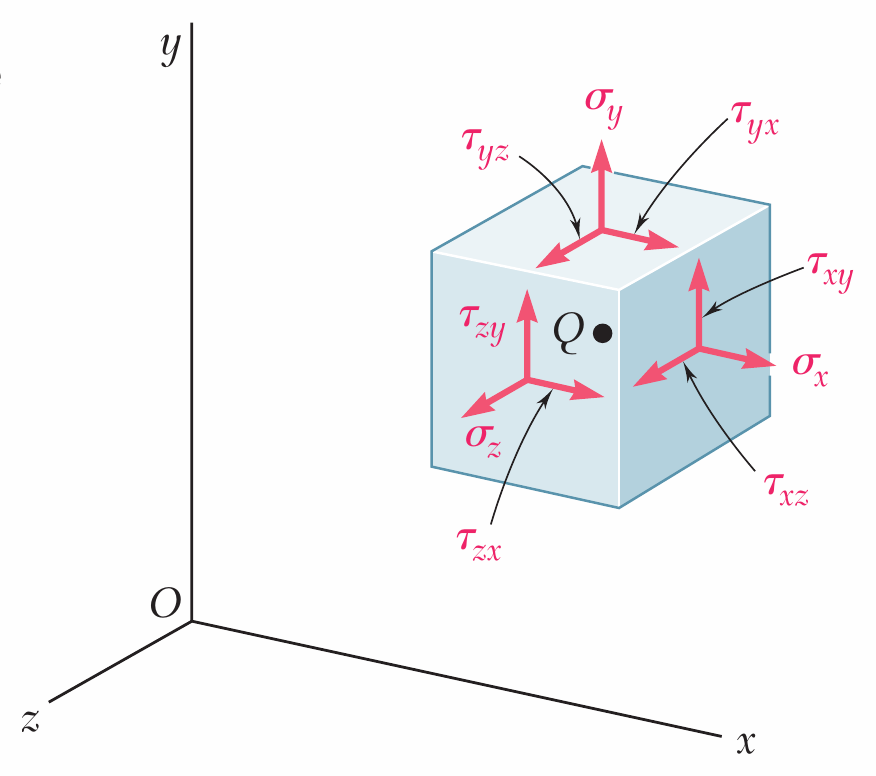
\includegraphics[width=\linewidth,height=2.9cm,keepaspectratio]{Chap_7/fig_7_1.png}\\[2pt]
      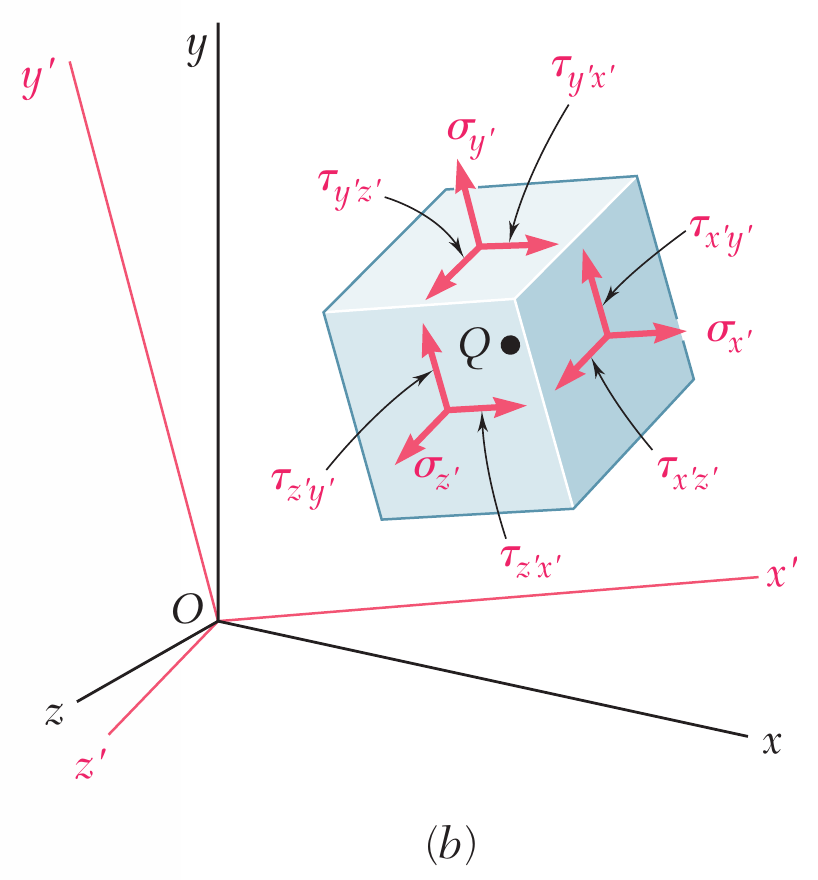
\includegraphics[width=\linewidth,height=2.9cm,keepaspectratio]{Chap_7/fig_7_1b.png}
  \end{columns}
\end{frame}
% ===========
\section{Trạng thái ứng suất phẳng}
\begin{frame}[t]{Giới thiệu: trạng thái ứng suất phẳng}
  \begin{columns}[T]
    \column{0.58\textwidth}
      \small
      \begin{itemize}
        \setlength{\itemsep}{0.7em}
        \item \textbf{Trạng thái ứng suất phẳng} -- trạng thái ứng suất trong
              đó hai mặt của phân tố lập phương không có ứng suất. Với ví dụ
              minh họa, trạng thái ứng suất được xác định bởi
              $\sigma_x$, $\sigma_y$, $\tau_{xy}$ và
              $\sigma_z = \tau_{zx} = \tau_{zy} = 0$.
        \item Trạng thái ứng suất phẳng xảy ra trong tấm mỏng chịu các lực
              tác dụng trong mặt phẳng giữa của tấm.
        \item Trạng thái ứng suất phẳng cũng xảy ra trên bề mặt tự do của cấu
              kiện kết cấu hoặc chi tiết máy, tức là tại mọi điểm trên bề mặt
              không chịu ngoại lực.
      \end{itemize}
    \column{0.40\textwidth}
      \centering
      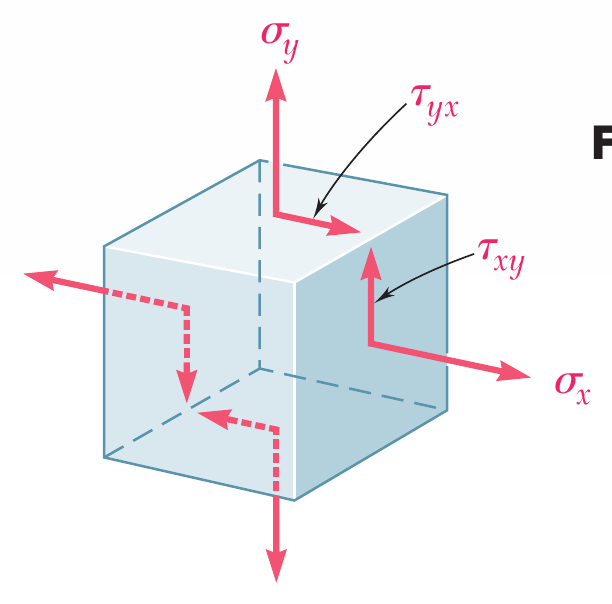
\includegraphics[width=\linewidth,height=1.9cm,keepaspectratio]{Chap_7/fig_7_2.png}\\[2pt]
      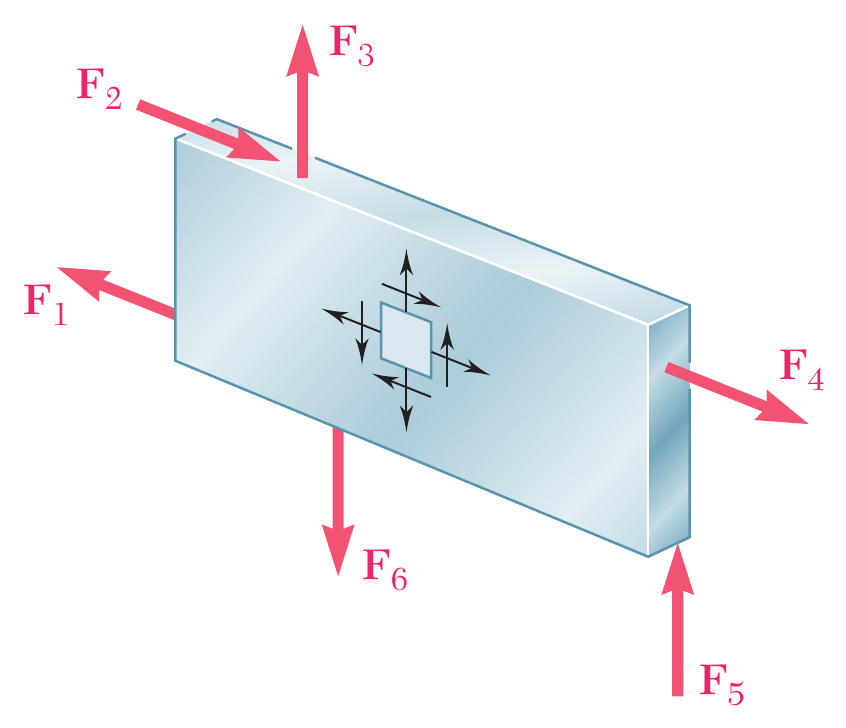
\includegraphics[width=\linewidth,height=1.9cm,keepaspectratio]{Chap_7/fig_7_3.png}\\[2pt]
      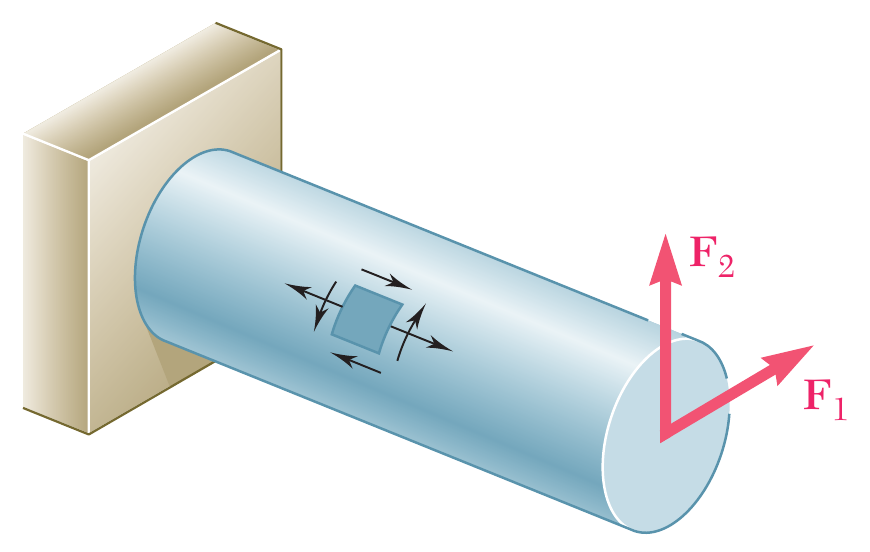
\includegraphics[width=\linewidth,height=1.9cm,keepaspectratio]{Chap_7/fig_7_4.png}
  \end{columns}
\end{frame}
% ===========
\section{Biến đổi ứng suất phẳng}
\begin{frame}[t]{Biến đổi ứng suất phẳng}
  \begin{columns}[T]
    \column{0.64\textwidth}
      \footnotesize
      \begin{itemize}
        \setlength{\itemsep}{0.3em}
        \item Xét điều kiện cân bằng của phân tố lăng trụ có các mặt vuông
              góc với các trục $x$, $y$ và $x'$:
      \end{itemize}
      \[
        \begin{aligned}
          \textstyle\sum F_{x'} = 0 &= \sigma_{x'}\Delta A
            - \sigma_x(\Delta A\cos\theta)\cos\theta
            - \tau_{xy}(\Delta A\cos\theta)\sin\theta\\
          &\quad - \sigma_y(\Delta A\sin\theta)\sin\theta
            - \tau_{xy}(\Delta A\sin\theta)\cos\theta\\
          \textstyle\sum F_{y'} = 0 &= \tau_{x'y'}\Delta A
            + \sigma_x(\Delta A\cos\theta)\sin\theta
            - \tau_{xy}(\Delta A\cos\theta)\cos\theta\\
          &\quad - \sigma_y(\Delta A\sin\theta)\cos\theta
            + \tau_{xy}(\Delta A\sin\theta)\sin\theta
        \end{aligned}
      \]
      \begin{itemize}
        \item Các phương trình có thể được viết lại thành:
      \end{itemize}
      \[
        \begin{aligned}
          \sigma_{x'} &= \frac{\sigma_x + \sigma_y}{2}
            + \frac{\sigma_x - \sigma_y}{2}\cos2\theta + \tau_{xy}\sin2\theta\\
          \sigma_{y'} &= \frac{\sigma_x + \sigma_y}{2}
            - \frac{\sigma_x - \sigma_y}{2}\cos2\theta - \tau_{xy}\sin2\theta\\
          \tau_{x'y'} &= -\frac{\sigma_x - \sigma_y}{2}\sin2\theta
            + \tau_{xy}\cos2\theta
        \end{aligned}
      \]
    \column{0.34\textwidth}
      \centering
      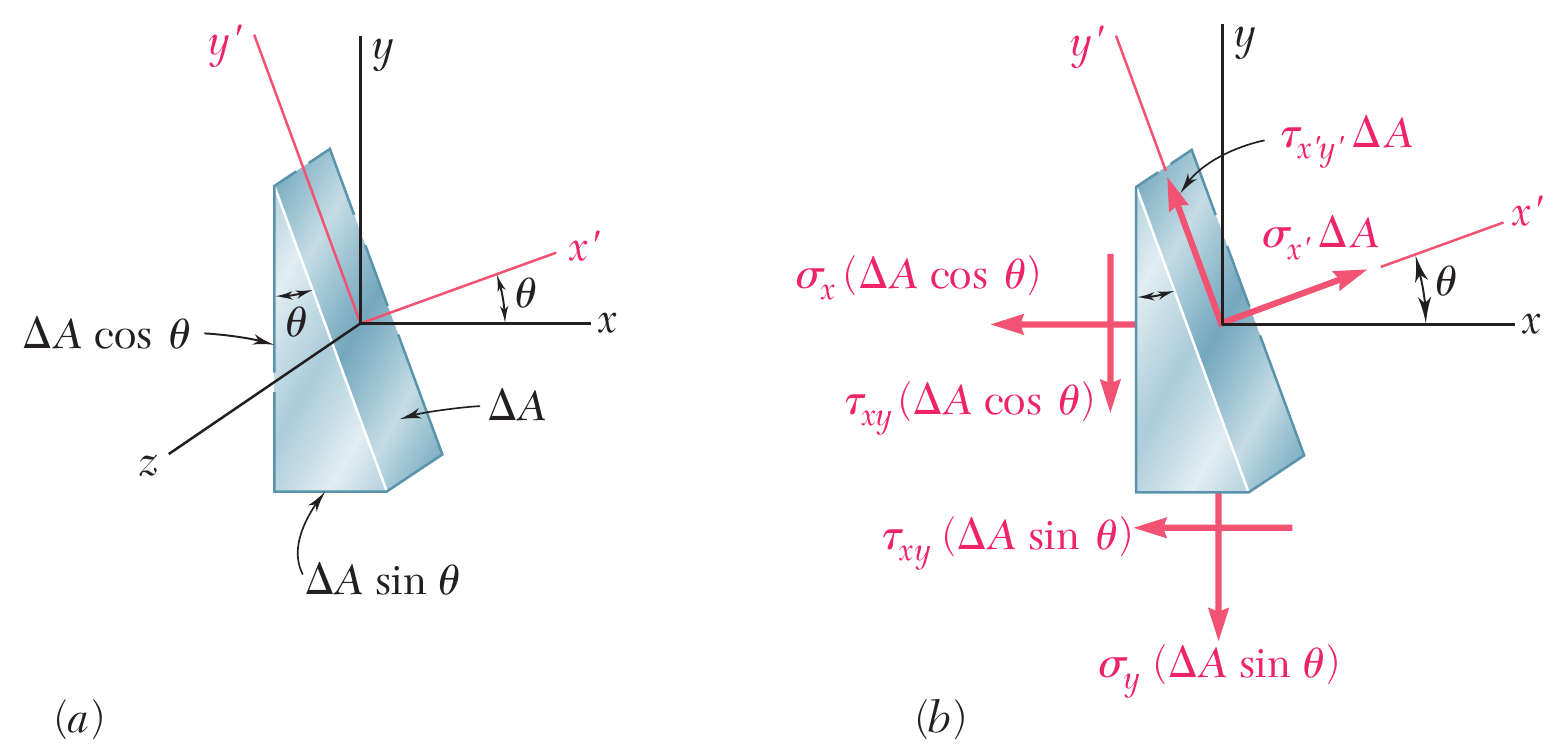
\includegraphics[width=\linewidth,height=5.5cm,keepaspectratio]{Chap_7/fig_7_6.png}
  \end{columns}
\end{frame}
% ===========
\section{Ứng suất chính}
\begin{frame}[t]{Ứng suất chính}
  \begin{columns}[T]
    \column{0.60\textwidth}
      \footnotesize
      \begin{itemize}
        \setlength{\itemsep}{0.20em}
        \item Kết hợp các phương trình trước để được phương trình tham số
              của một đường tròn:
        \[
          \left(\sigma_{x'} - \sigma_{\mathrm{tb}}\right)^2 + \tau_{x'y'}^2 = R^2
        \]
        trong đó
        \[
          \sigma_{\mathrm{tb}} = \frac{\sigma_x + \sigma_y}{2}
          \qquad
          R = \sqrt{\left(\frac{\sigma_x - \sigma_y}{2}\right)^2 + \tau_{xy}^2}
        \]
        \item Ứng suất chính xuất hiện trên các mặt chính, nơi ứng suất tiếp
              bằng không:
        \[
          \tan2\theta_p = \frac{2\tau_{xy}}{\sigma_x - \sigma_y}
        \]
        \[
          \sigma_{\max,\min} = \frac{\sigma_x + \sigma_y}{2}
            \pm\sqrt{\left(\frac{\sigma_x - \sigma_y}{2}\right)^2 + \tau_{xy}^2}
        \]
        Lưu ý: phương trình xác định hai góc cách nhau $90^\circ$.
      \end{itemize}
    \column{0.38\textwidth}
      \centering
      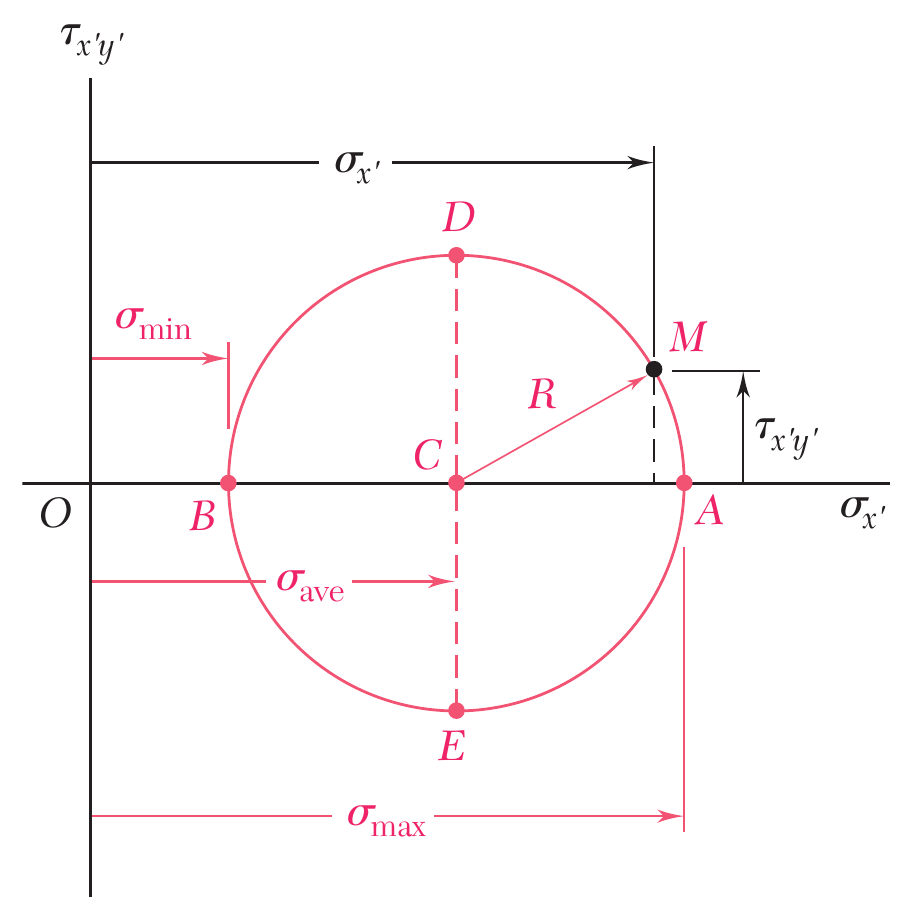
\includegraphics[width=\linewidth,height=2.5cm,keepaspectratio]{Chap_7/fig_7_7.png}\\[2pt]
      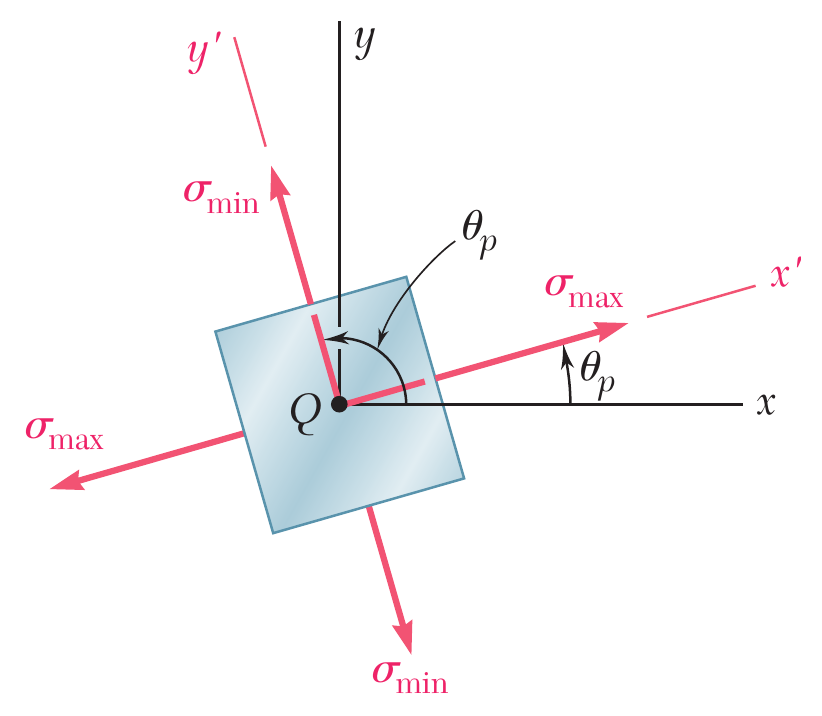
\includegraphics[width=\linewidth,height=2.5cm,keepaspectratio]{Chap_7/fig_7_9.png}
  \end{columns}
\end{frame}
% ===========
\section{Ứng suất tiếp lớn nhất}
\begin{frame}[t]{Ứng suất tiếp lớn nhất}
  \begin{columns}[T]
    \column{0.58\textwidth}
      \small
      Ứng suất tiếp lớn nhất xảy ra khi $\sigma_{x'} = \sigma_{\mathrm{tb}}$:
      \[
        \tau_{\max} = R = \sqrt{\left(\frac{\sigma_x - \sigma_y}{2}\right)^2 + \tau_{xy}^2}
      \]
      \[
        \tan2\theta_s = -\frac{\sigma_x - \sigma_y}{2\tau_{xy}}
      \]
      Lưu ý: phương trình xác định hai góc cách nhau $90^\circ$ và lệch
      $45^\circ$ so với $\theta_p$.
      \[
        \sigma' = \sigma_{\mathrm{tb}} = \frac{\sigma_x + \sigma_y}{2}
      \]
    \column{0.40\textwidth}
      \centering
      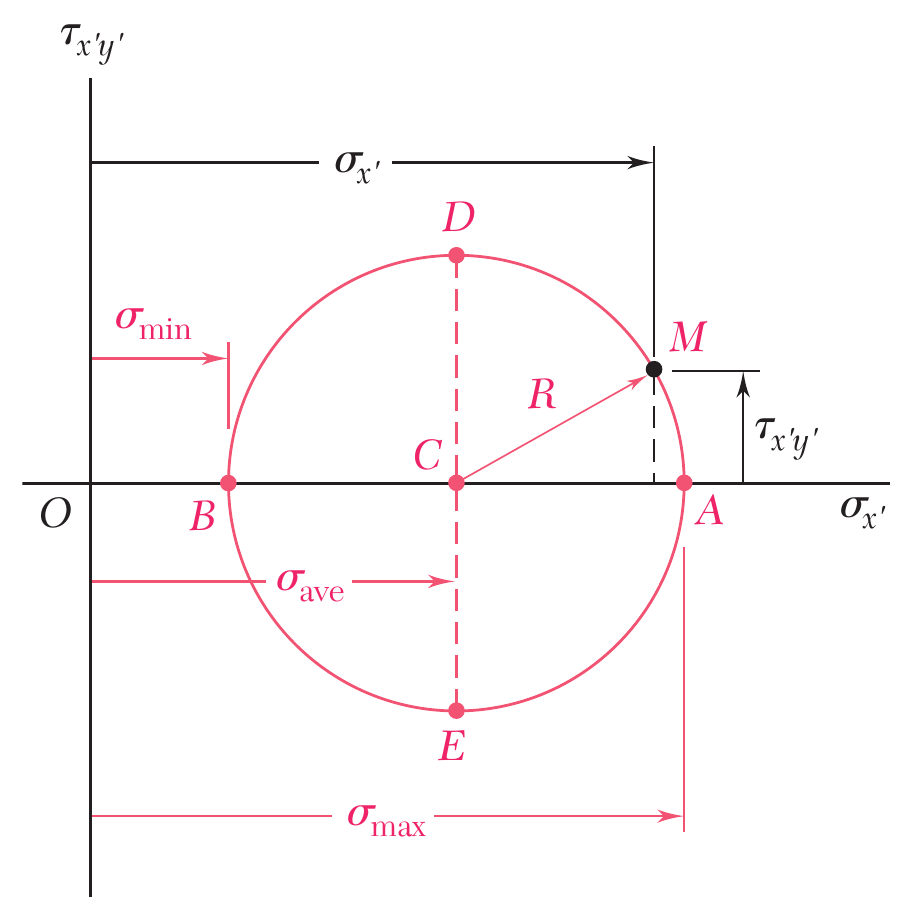
\includegraphics[width=\linewidth,height=2.9cm,keepaspectratio]{Chap_7/fig_7_7.png}\\[2pt]
      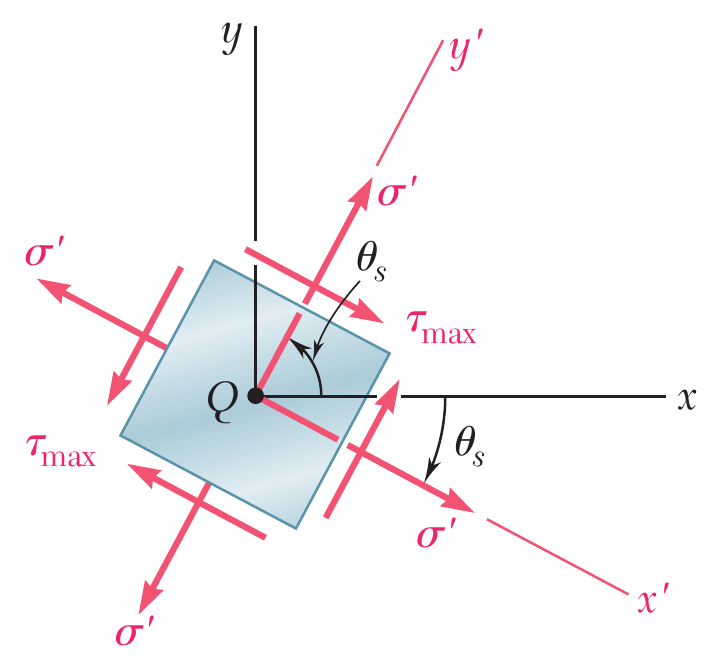
\includegraphics[width=\linewidth,height=2.9cm,keepaspectratio]{Chap_7/fig_7_10.png}
  \end{columns}
\end{frame}
% ===========
\section{Ví dụ 7.01}
\begin{frame}[t]{Ví dụ 7.01}
  \begin{columns}[T]
    \column{0.40\textwidth}
      \centering
      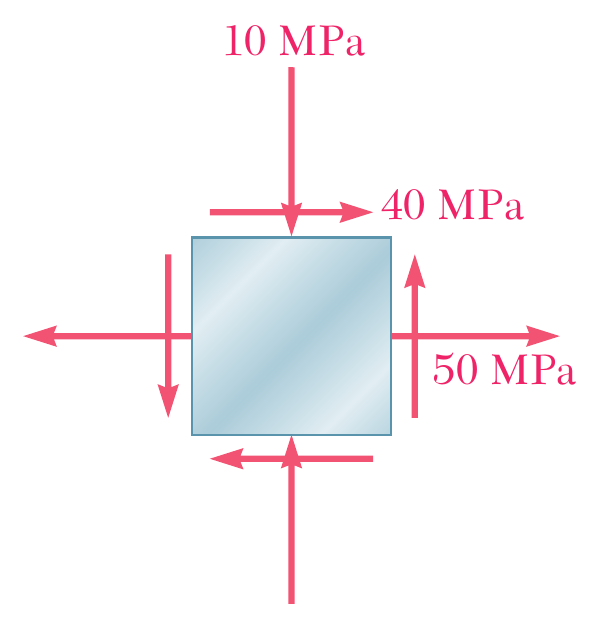
\includegraphics[width=\linewidth,height=4.1cm,keepaspectratio]{Chap_7/fig_7_11.png}\\
      \tiny Hình 7.13
    \column{0.58\textwidth}
      \footnotesize
      Với trạng thái ứng suất phẳng như hình vẽ, xác định (a) các mặt chính,
      (b) các ứng suất chính, (c) ứng suất tiếp lớn nhất và ứng suất pháp
      tương ứng.

      \vspace{0.5em}
      \textbf{LỜI GIẢI:}
      \begin{itemize}
        \setlength{\itemsep}{0.15em}
        \item Tìm hướng của phân tố ứng với ứng suất chính từ:
        \[
          \tan2\theta_p = \frac{2\tau_{xy}}{\sigma_x - \sigma_y}
        \]
        \item Xác định các ứng suất chính từ:
        \[
          \sigma_{\max,\min} = \frac{\sigma_x + \sigma_y}{2}
            \pm\sqrt{\left(\frac{\sigma_x - \sigma_y}{2}\right)^2 + \tau_{xy}^2}
        \]
        \item Tính ứng suất tiếp lớn nhất và ứng suất pháp tương ứng:
        \[
          \tau_{\max} = \sqrt{\left(\frac{\sigma_x - \sigma_y}{2}\right)^2 + \tau_{xy}^2}
          \qquad
          \sigma' = \frac{\sigma_x + \sigma_y}{2}
        \]
      \end{itemize}
  \end{columns}
\end{frame}
% ===========
\begin{frame}[t]{Ví dụ 7.01 (tiếp)}
  \begin{columns}[T]
    \column{0.60\textwidth}
      \small
      $\sigma_x = +50\,\mathrm{MPa}$, \quad $\sigma_y = -10\,\mathrm{MPa}$,
      \quad $\tau_{xy} = +40\,\mathrm{MPa}$

      \vspace{0.3em}
      \textbf{LỜI GIẢI:}
      \begin{itemize}
        \setlength{\itemsep}{0.4em}
        \item Tìm hướng của phân tố ứng với ứng suất chính:
        \[
          \tan2\theta_p = \frac{2\tau_{xy}}{\sigma_x - \sigma_y}
            = \frac{2(+40)}{50 - (-10)} = 1{,}333
        \]
        \[
          2\theta_p = 53{,}1^\circ,\ 233{,}1^\circ
          \qquad \theta_p = 26{,}6^\circ,\ 116{,}6^\circ
        \]
        \item Xác định các ứng suất chính:
        \[
          \sigma_{\max,\min} = \frac{\sigma_x + \sigma_y}{2}
            \pm\sqrt{\left(\frac{\sigma_x - \sigma_y}{2}\right)^2 + \tau_{xy}^2}
        \]
        \[
          \sigma_{\max,\min} = 20 \pm\sqrt{(30)^2 + (40)^2}
        \]
        \[
          \boxed{\sigma_{\max} = 70\,\mathrm{MPa} \qquad \sigma_{\min} = -30\,\mathrm{MPa}}
        \]
      \end{itemize}
    \column{0.38\textwidth}
      \centering
      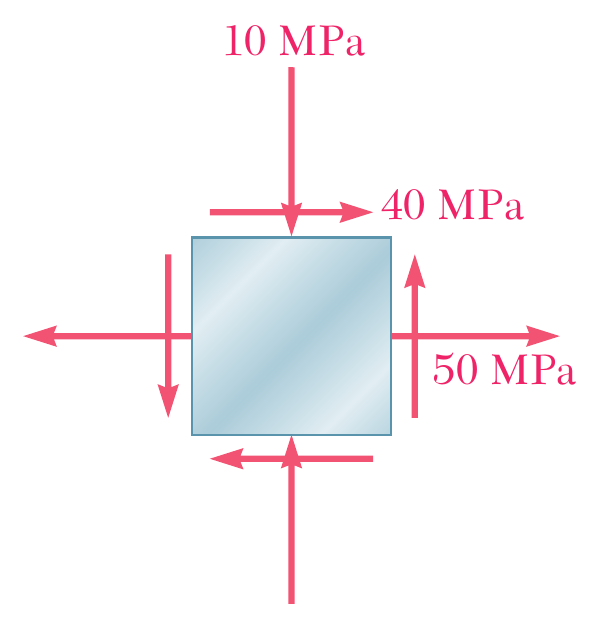
\includegraphics[width=\linewidth,height=2.6cm,keepaspectratio]{Chap_7/fig_7_11.png}\\
      \scriptsize Hình 7.13\\[2pt]
      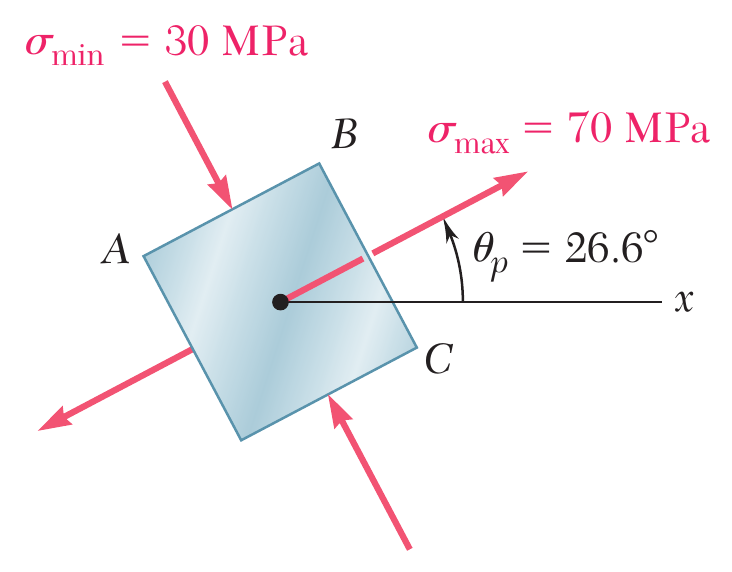
\includegraphics[width=\linewidth,height=2.6cm,keepaspectratio]{Chap_7/fig_7_12.png}\\
      \scriptsize Hình 7.14
  \end{columns}
\end{frame}
% ===========
\begin{frame}[t]{Ví dụ 7.01 (tiếp)}
  \begin{columns}[T]
    \column{0.60\textwidth}
      \small
      \begin{itemize}
        \setlength{\itemsep}{0.5em}
        \item Tính ứng suất tiếp lớn nhất:
        \[
          \tau_{\max} = \sqrt{\left(\frac{\sigma_x - \sigma_y}{2}\right)^2 + \tau_{xy}^2}
            = \sqrt{(30)^2 + (40)^2}
        \]
        \[
          \boxed{\tau_{\max} = 50\,\mathrm{MPa}}
        \]
        \[
          \theta_s = \theta_p - 45^\circ
          \qquad \boxed{\theta_s = -18{,}4^\circ,\ 71{,}6^\circ}
        \]
        \item Ứng suất pháp tương ứng:
        \[
          \sigma' = \sigma_{\mathrm{tb}} = \frac{\sigma_x + \sigma_y}{2}
            = \frac{50 - 10}{2}
          \qquad \boxed{\sigma' = 20\,\mathrm{MPa}}
        \]
      \end{itemize}
    \column{0.38\textwidth}
      \centering
      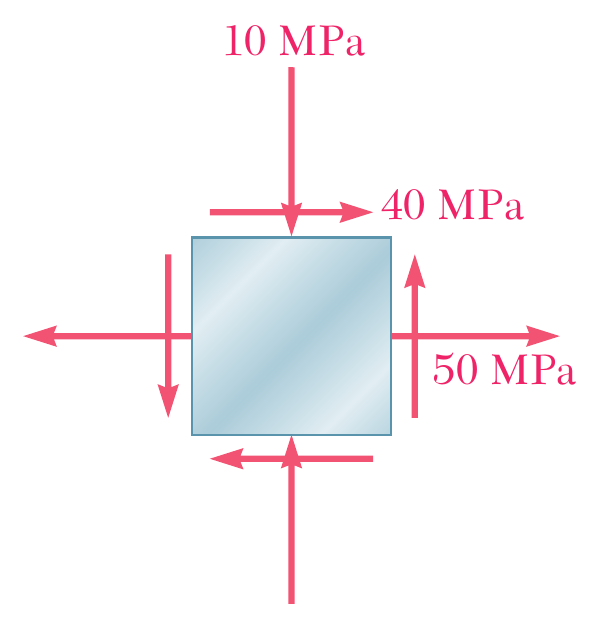
\includegraphics[width=\linewidth,height=2.6cm,keepaspectratio]{Chap_7/fig_7_11.png}\\
      \scriptsize Hình 7.13\\[2pt]
      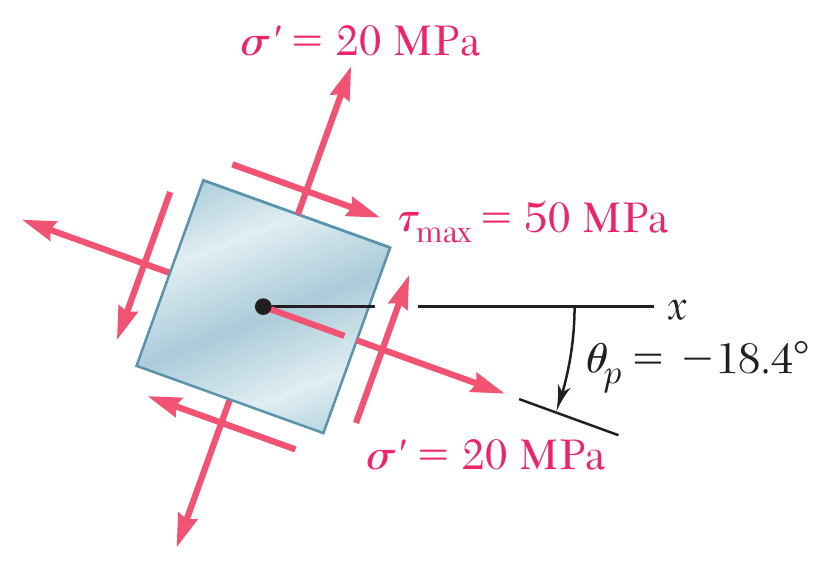
\includegraphics[width=\linewidth,height=2.6cm,keepaspectratio]{Chap_7/fig_7_14.png}\\
      \scriptsize Hình 7.16
  \end{columns}
\end{frame}
% ===========
\section{Bài mẫu 7.1}
\begin{frame}[t]{Bài mẫu 7.1}
  \begin{columns}[T]
    \column{0.42\textwidth}
      \centering
      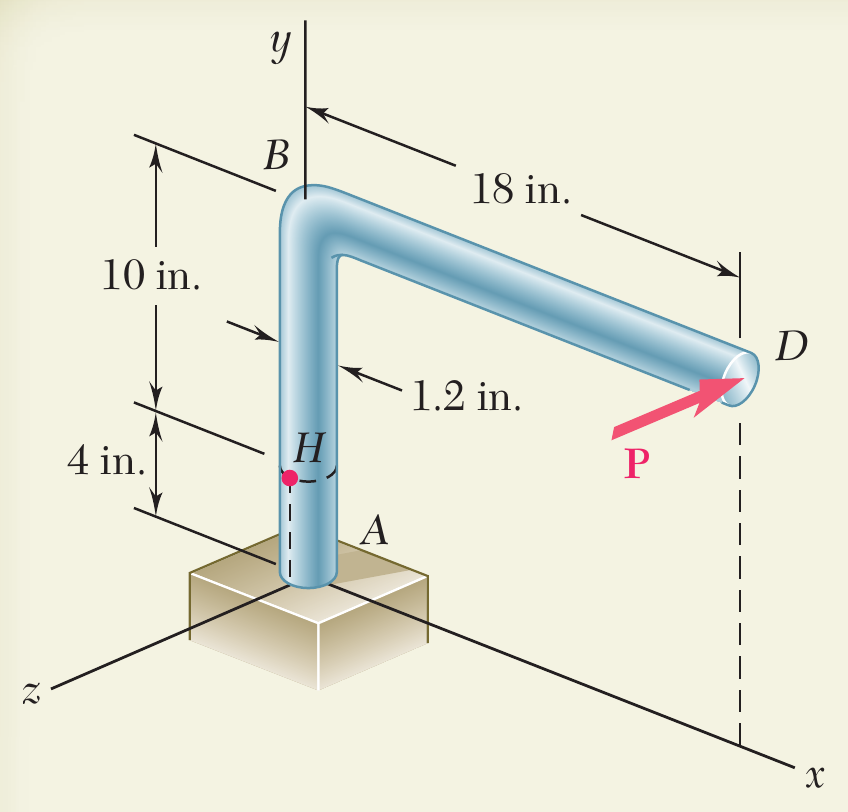
\includegraphics[width=\linewidth,height=5.5cm,keepaspectratio]{Chap_7/sp_7_1_a.png}
    \column{0.56\textwidth}
      \small
      Một lực nằm ngang $P$ có độ lớn 600 N tác dụng vào đầu $D$ của tay đòn
      $ABD$. Xác định (a) ứng suất pháp và ứng suất tiếp trên phân tố tại
      điểm $H$ có các cạnh song song với các trục $x$ và $y$, (b) các mặt
      chính và ứng suất chính tại điểm $H$.

      \vspace{0.5em}
      \textbf{LỜI GIẢI:}
      \begin{itemize}
        \setlength{\itemsep}{0.4em}
        \item Xác định hệ lực -- ngẫu lực tương đương tại tâm mặt cắt ngang
              đi qua $H$.
        \item Tính ứng suất pháp và ứng suất tiếp tại $H$.
        \item Xác định các mặt chính và tính các ứng suất chính.
      \end{itemize}
  \end{columns}
\end{frame}
% ===========
\begin{frame}[t]{Bài mẫu 7.1 (tiếp)}
  \begin{columns}[T]
    \column{0.58\textwidth}
      \small
      \textbf{LỜI GIẢI:}
      \begin{itemize}
        \setlength{\itemsep}{0.4em}
        \item Xác định hệ lực -- ngẫu lực tương đương tại tâm mặt cắt ngang
              đi qua $H$:
        \[
          P = 600\,\mathrm{N}
        \]
        \[
          T = (600\,\mathrm{N})(0{,}45\,\mathrm{m}) = 270\,\mathrm{N\cdot m}
        \]
        \[
          M_x = (600\,\mathrm{N})(0{,}25\,\mathrm{m}) = 150\,\mathrm{N\cdot m}
        \]
        \item Tính ứng suất pháp và ứng suất tiếp tại $H$:
        \[
          \sigma_y = +\frac{Mc}{I}
            = +\frac{(150\,\mathrm{N\cdot m})(0{,}015\,\mathrm{m})}{\frac{1}{4}\pi(0{,}015\,\mathrm{m})^4}
        \]
        \[
          \tau_{xy} = +\frac{Tc}{J}
            = +\frac{(270\,\mathrm{N\cdot m})(0{,}015\,\mathrm{m})}{\frac{1}{2}\pi(0{,}015\,\mathrm{m})^4}
        \]
        \[
          \sigma_x = 0 \qquad \sigma_y = +56{,}6\,\mathrm{MPa} \qquad
          \tau_{xy} = +50{,}9\,\mathrm{MPa}
        \]
      \end{itemize}
    \column{0.40\textwidth}
      \centering
      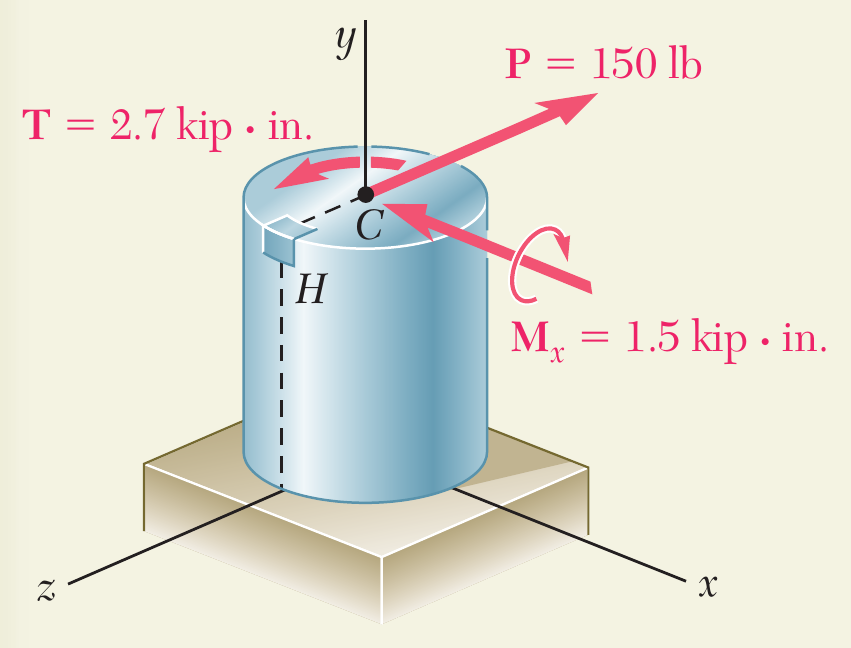
\includegraphics[width=\linewidth,height=2.9cm,keepaspectratio]{Chap_7/sp_7_1_b.png}\\[2pt]
      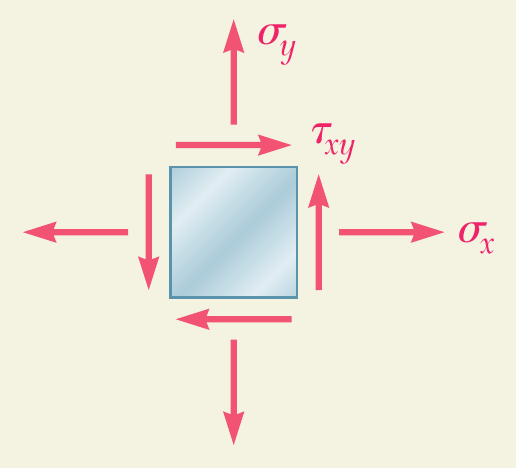
\includegraphics[width=\linewidth,height=2.9cm,keepaspectratio]{Chap_7/sp_7_1_c.png}
  \end{columns}
\end{frame}
% ===========
\begin{frame}[t]{Bài mẫu 7.1 (tiếp)}
  \begin{columns}[T]
    \column{0.60\textwidth}
      \small
      \begin{itemize}
        \setlength{\itemsep}{0.4em}
        \item Xác định các mặt chính và tính các ứng suất chính:
        \[
          \tan2\theta_p = \frac{2\tau_{xy}}{\sigma_x - \sigma_y}
            = \frac{2(50{,}9)}{0 - 56{,}6} = -1{,}8
        \]
        \[
          2\theta_p = -61{,}0^\circ,\ 119^\circ
          \qquad \theta_p = -30{,}5^\circ,\ 59{,}5^\circ
        \]
        \[
          \sigma_{\max,\min} = \frac{\sigma_x + \sigma_y}{2}
            \pm\sqrt{\left(\frac{\sigma_x - \sigma_y}{2}\right)^2 + \tau_{xy}^2}
        \]
        \[
          = \frac{0 + 56{,}6}{2} \pm\sqrt{\left(\frac{0 - 56{,}6}{2}\right)^2 + (50{,}9)^2}
        \]
        \[
          \boxed{\sigma_{\max} = +86{,}5\,\mathrm{MPa} \qquad
                 \sigma_{\min} = -29{,}9\,\mathrm{MPa}}
        \]
      \end{itemize}
    \column{0.38\textwidth}
      \centering
      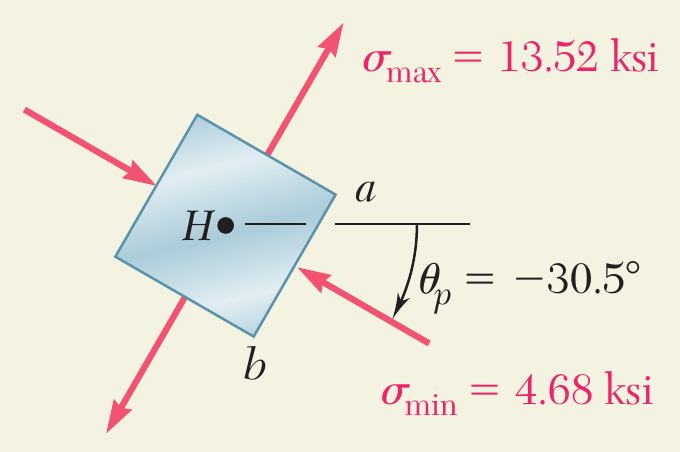
\includegraphics[width=\linewidth,height=5.5cm,keepaspectratio]{Chap_7/sp_7_1_d.png}
  \end{columns}
\end{frame}
% ===========
\section{Vòng tròn Mohr cho trạng thái ứng suất phẳng}
\begin{frame}[t]{Vòng tròn Mohr cho trạng thái ứng suất phẳng}
  \begin{columns}[T]
    \column{0.60\textwidth}
      \small
      \begin{itemize}
        \setlength{\itemsep}{0.4em}
        \item Sau khi đã xác lập ý nghĩa vật lý của vòng tròn Mohr cho trạng
              thái ứng suất phẳng, có thể áp dụng nó với các xem xét hình học
              đơn giản. Các giá trị tới hạn được ước lượng bằng đồ thị hoặc
              tính toán.
        \item Với trạng thái ứng suất phẳng đã biết $\sigma_x$, $\sigma_y$,
              $\tau_{xy}$, vẽ các điểm $X$, $Y$ và dựng đường tròn tâm $C$:
        \[
          \sigma_{\mathrm{tb}} = \frac{\sigma_x + \sigma_y}{2}
          \qquad
          R = \sqrt{\left(\frac{\sigma_x - \sigma_y}{2}\right)^2 + \tau_{xy}^2}
        \]
        \item Các ứng suất chính nhận được tại $A$ và $B$:
        \[
          \sigma_{\max,\min} = \sigma_{\mathrm{tb}} \pm R
          \qquad
          \tan2\theta_p = \frac{2\tau_{xy}}{\sigma_x - \sigma_y}
        \]
        Chiều quay từ $Ox$ đến $Oa$ cùng chiều với chiều quay từ $CX$ đến
        $CA$.
      \end{itemize}
    \column{0.38\textwidth}
      \centering
      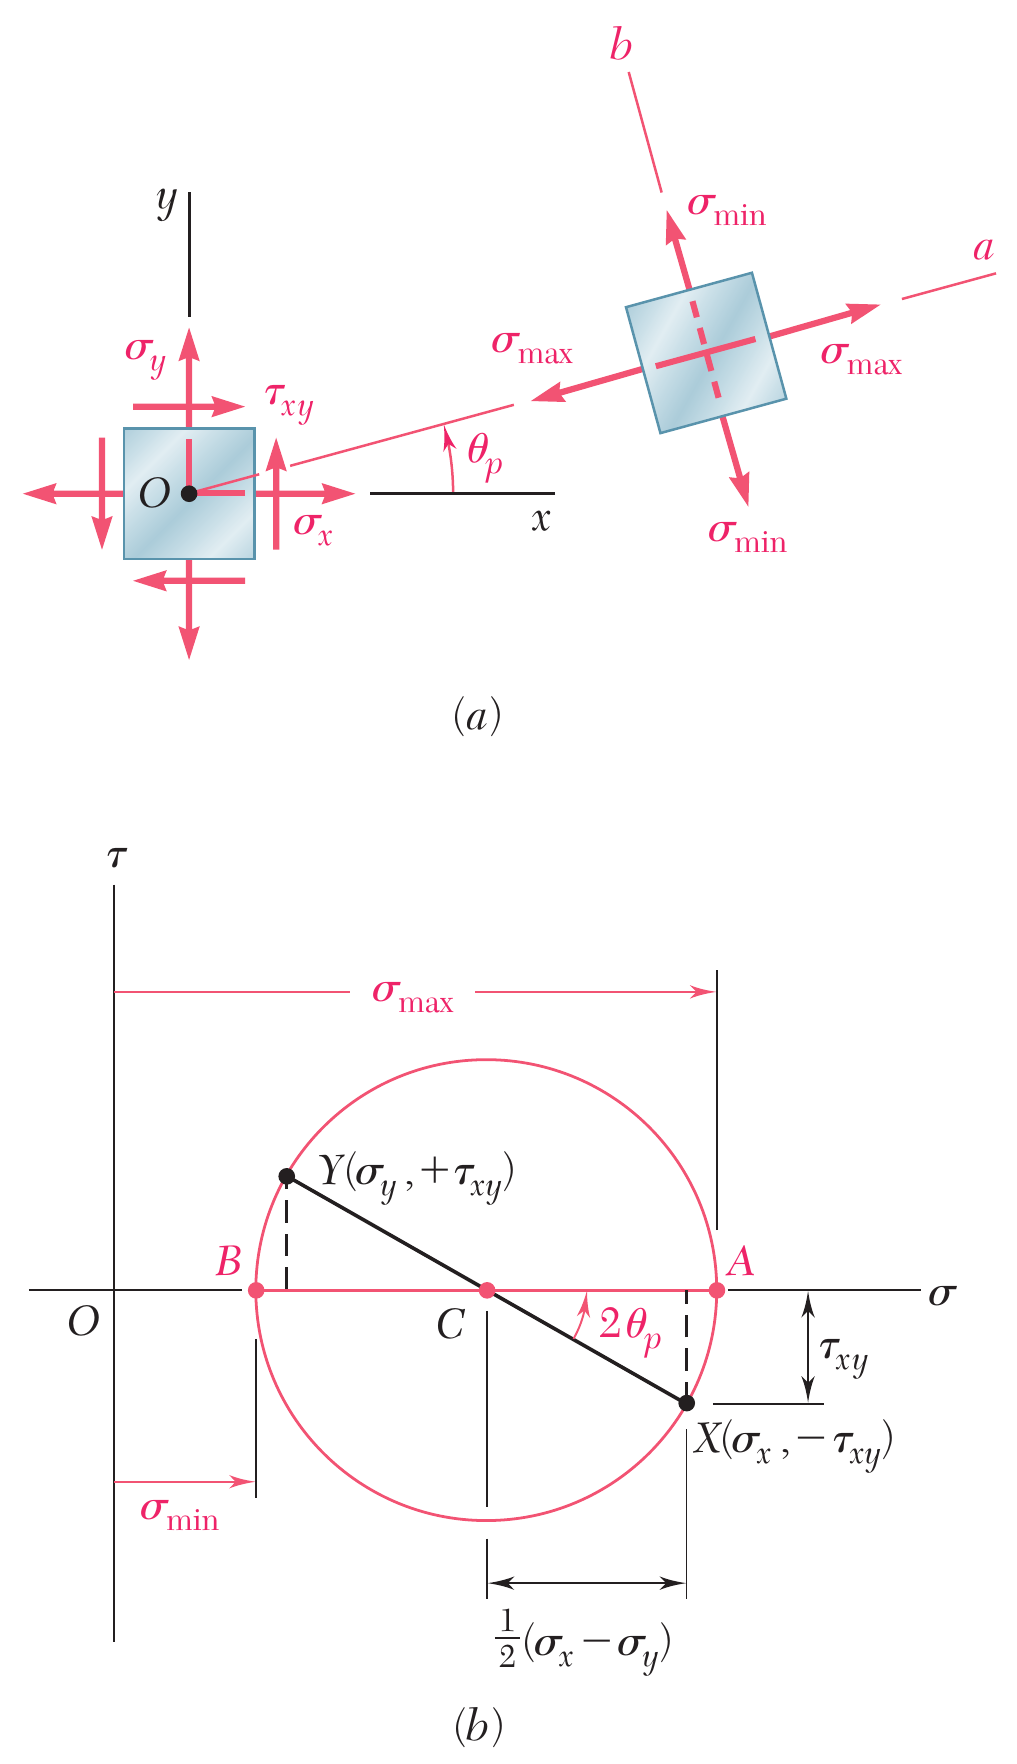
\includegraphics[width=\linewidth,height=2.9cm,keepaspectratio]{Chap_7/fig_7_15.png}\\[2pt]
      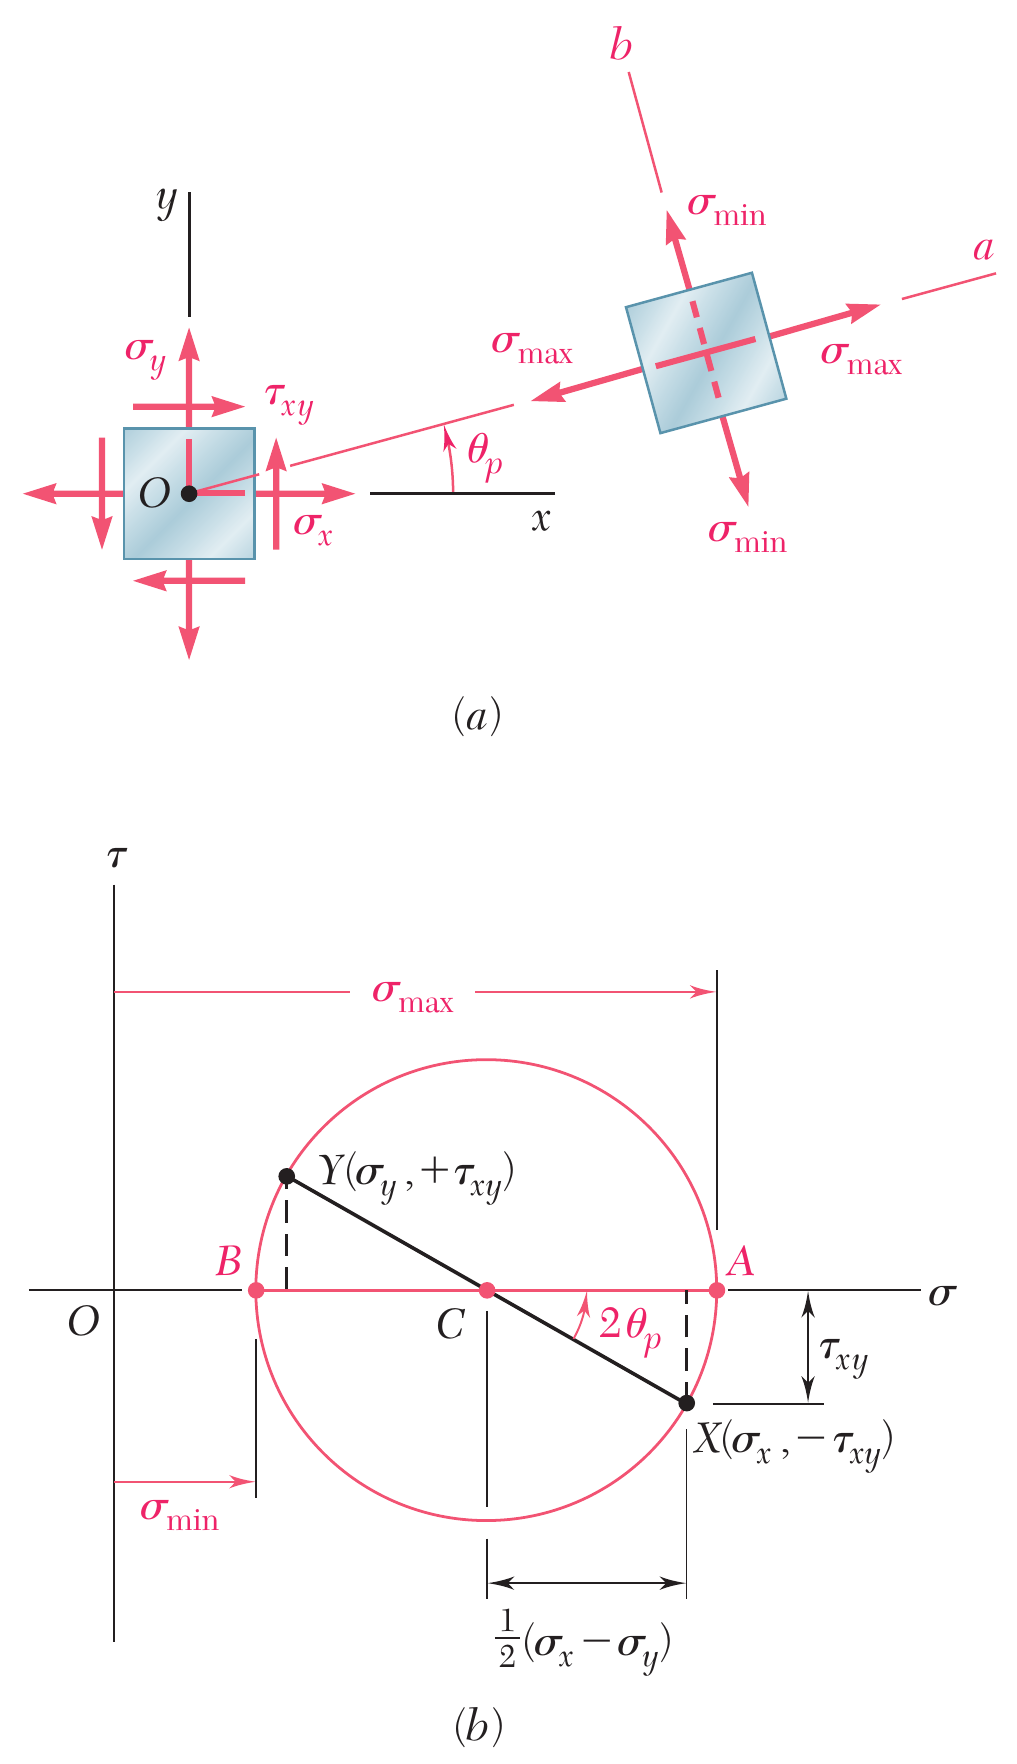
\includegraphics[width=\linewidth,height=2.9cm,keepaspectratio]{Chap_7/fig_7_15.png}
  \end{columns}
\end{frame}
% ===========
\begin{frame}[t]{Vòng tròn Mohr cho trạng thái ứng suất phẳng (tiếp)}
  \begin{columns}[T]
    \column{0.56\textwidth}
      \small
      \begin{itemize}
        \setlength{\itemsep}{0.9em}
        \item Khi vòng tròn Mohr đã được xác định duy nhất, có thể biểu diễn
              trạng thái ứng suất theo các hướng trục khác.
        \item Với trạng thái ứng suất tại góc $\theta$ so với hệ trục $xy$,
              dựng đường kính mới $X'Y'$ hợp với $XY$ một góc $2\theta$.
        \item Ứng suất pháp và ứng suất tiếp nhận được từ tọa độ của $X'$
              và $Y'$.
      \end{itemize}
    \column{0.42\textwidth}
      \centering
      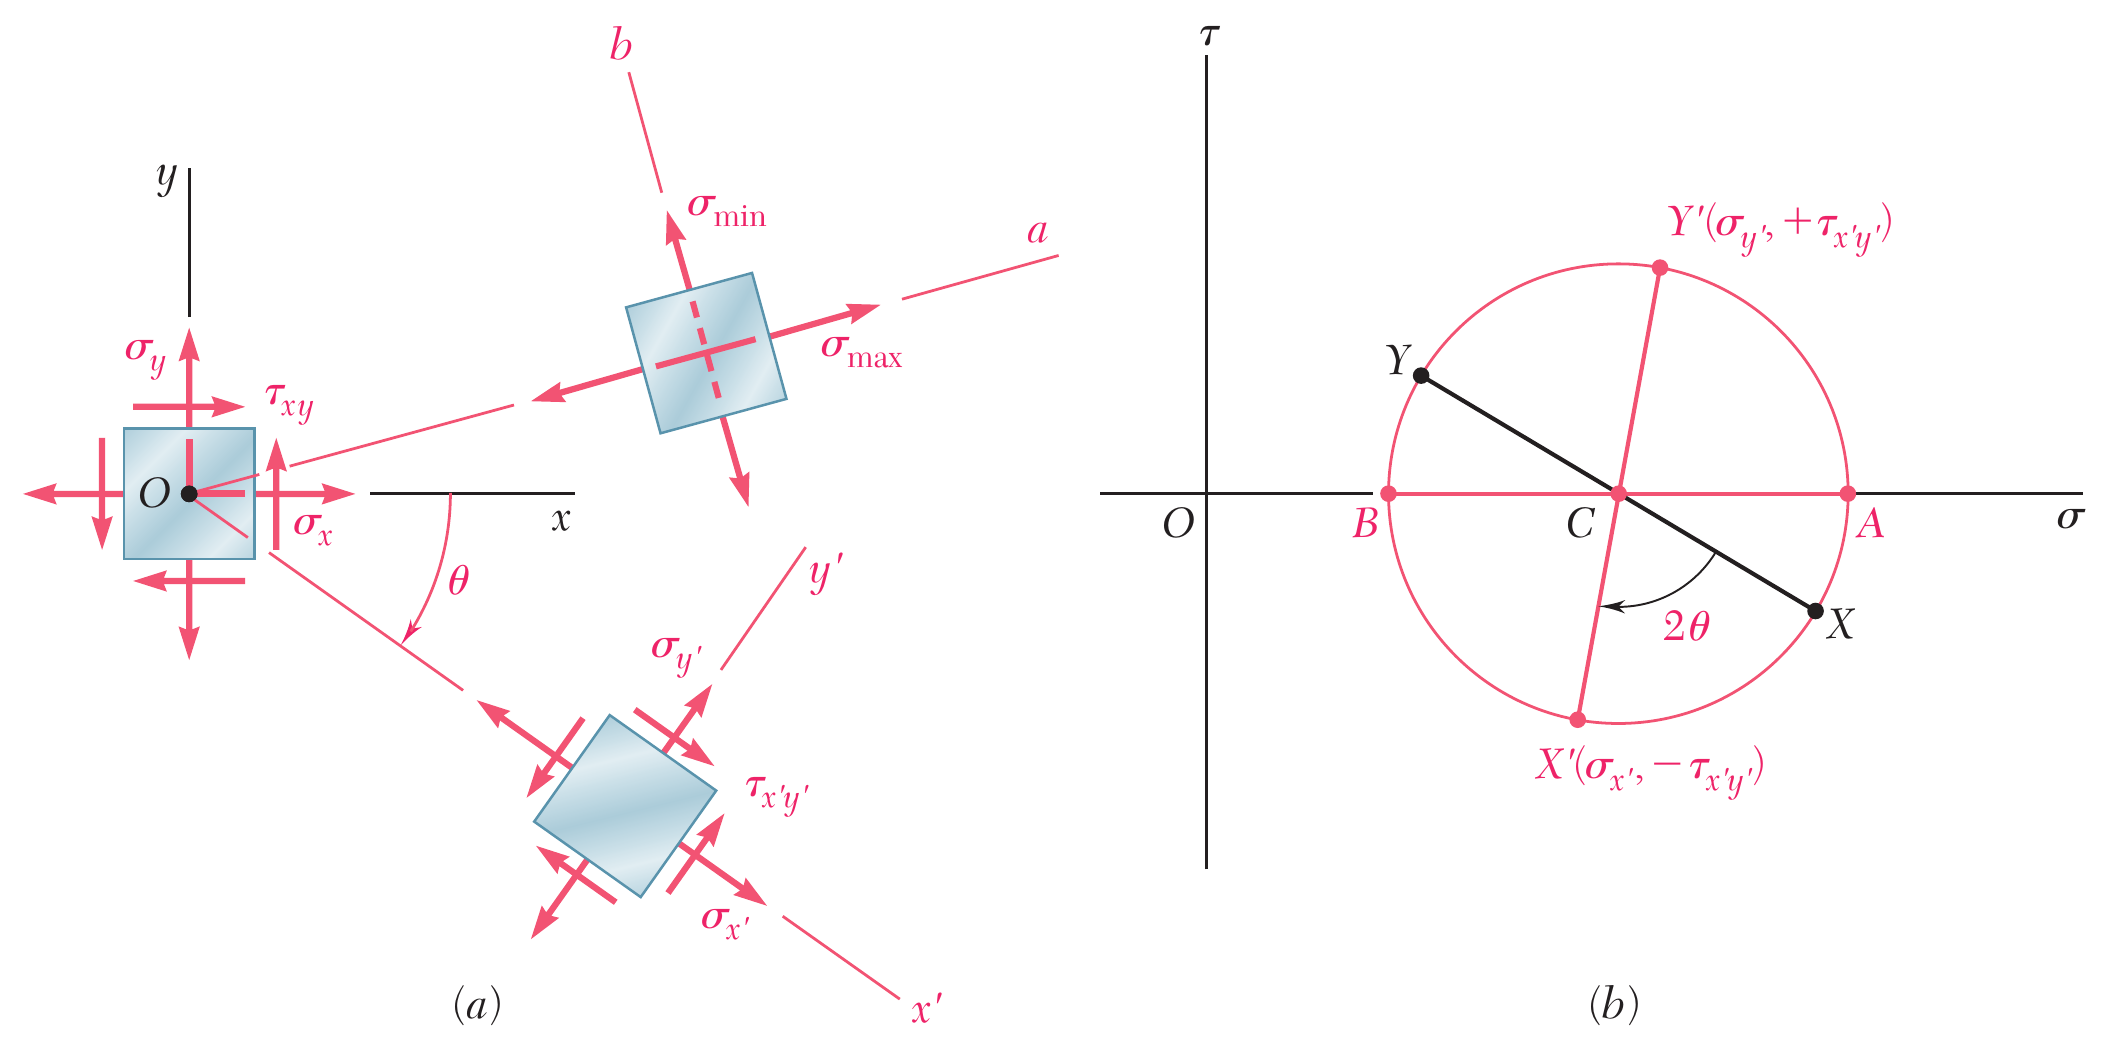
\includegraphics[width=\linewidth,height=5.5cm,keepaspectratio]{Chap_7/fig_7_16.png}
  \end{columns}
\end{frame}
% ===========
\begin{frame}[t]{Vòng tròn Mohr cho trạng thái ứng suất phẳng (tiếp)}
  \begin{columns}[T]
    \column{0.49\textwidth}
      \small
      Vòng tròn Mohr cho tải trọng dọc trục đúng tâm:
      \[
        \sigma_x = \frac{P}{A}, \quad \sigma_y = \tau_{xy} = 0
      \]
      \[
        \sigma_{x'} = \sigma_{y'} = \tau_{x'y'} = \frac{P}{2A}
      \]
      \centering
      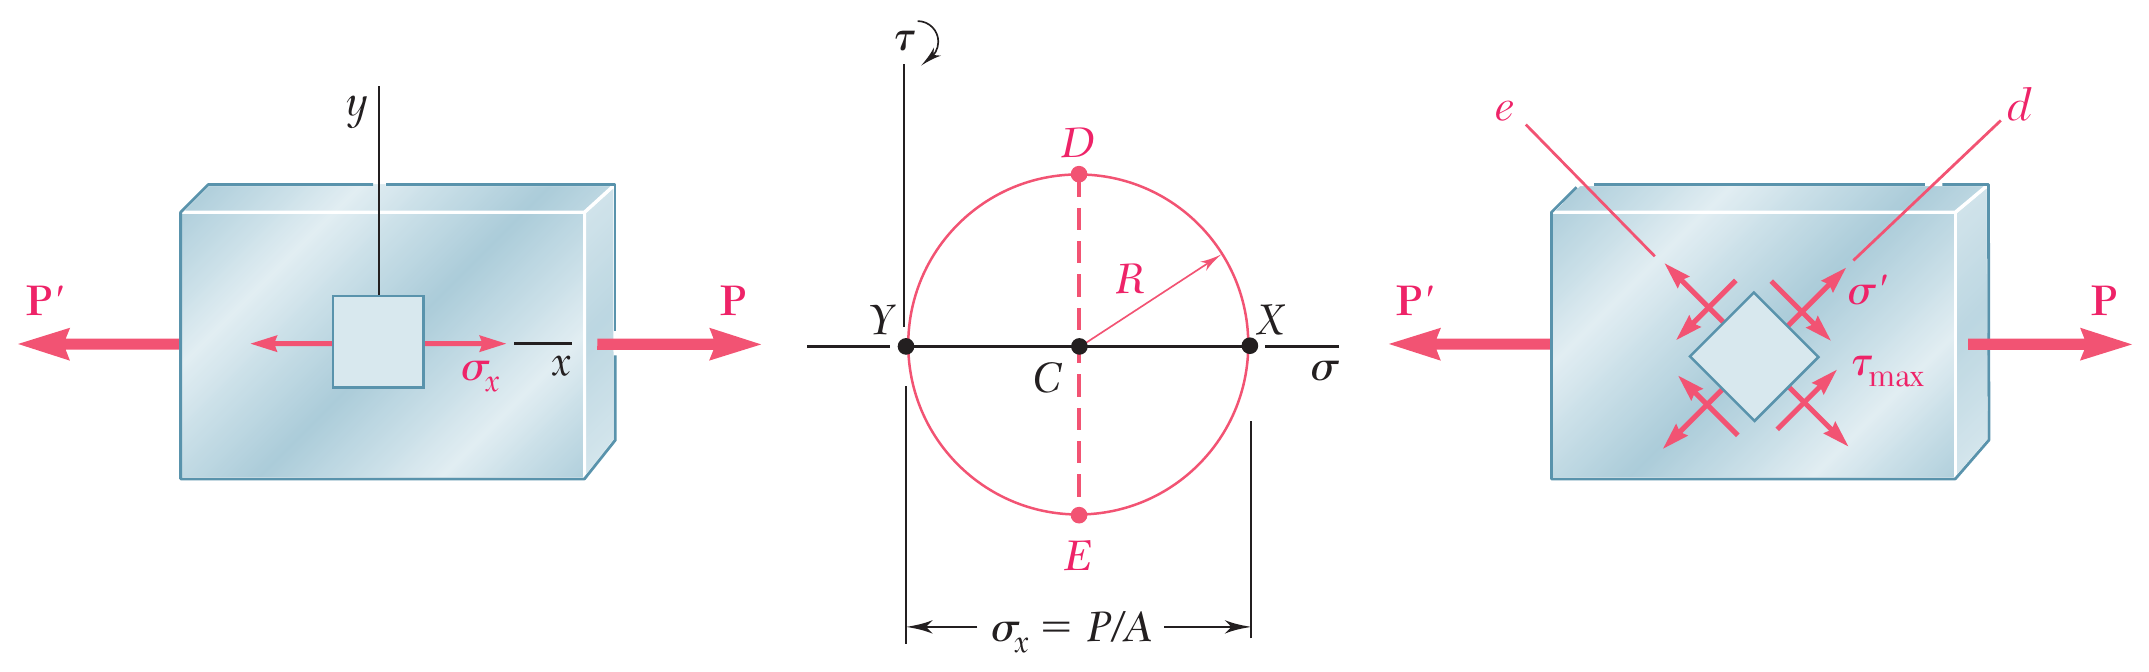
\includegraphics[width=\linewidth,height=3.2cm,keepaspectratio]{Chap_7/fig_7_21.png}
    \column{0.49\textwidth}
      \small
      Vòng tròn Mohr cho tải trọng xoắn:
      \[
        \sigma_x = \sigma_y = 0, \quad \tau_{xy} = \frac{Tc}{J}
      \]
      \[
        \sigma_{x'} = -\sigma_{y'} = \frac{Tc}{J}, \quad \tau_{x'y'} = 0
      \]
      \centering
      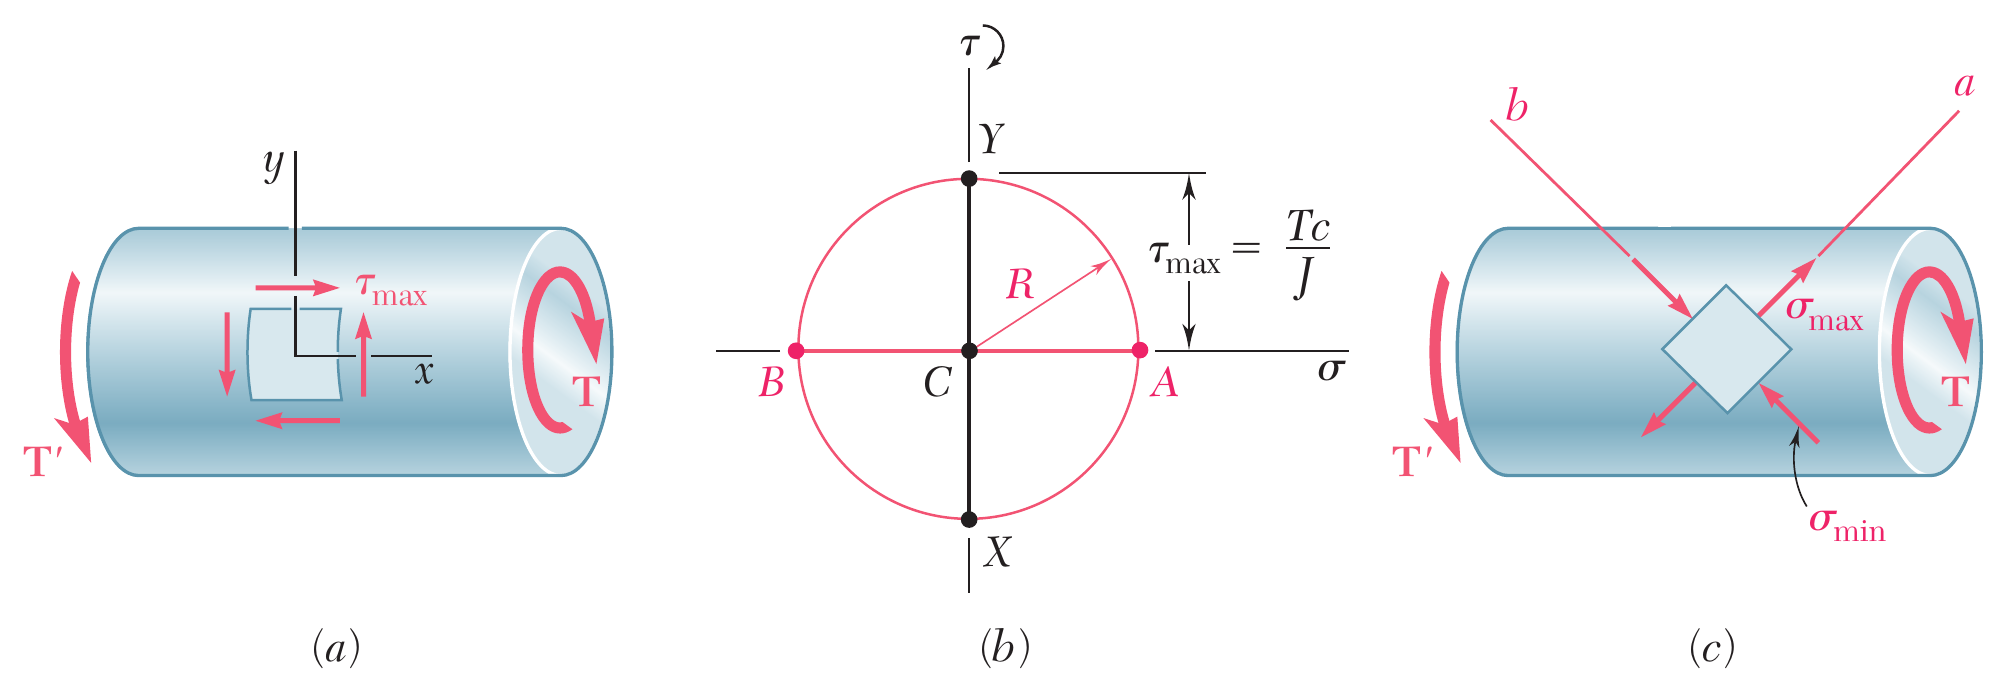
\includegraphics[width=\linewidth,height=3.2cm,keepaspectratio]{Chap_7/fig_7_22.png}
  \end{columns}
\end{frame}
% ===========
\section{Ví dụ 7.02}
\begin{frame}[t]{Ví dụ 7.02}
  \begin{columns}[T]
    \column{0.40\textwidth}
      \centering
      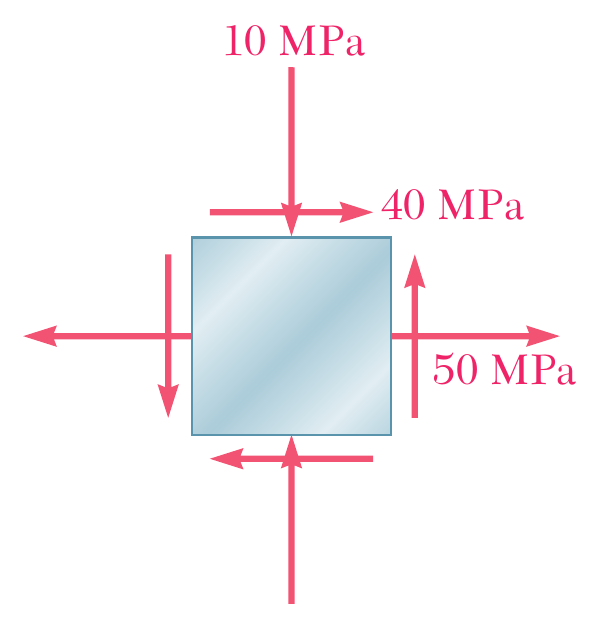
\includegraphics[width=\linewidth,height=2.6cm,keepaspectratio]{Chap_7/fig_7_11.png}\\
      \scriptsize Hình 7.13\\[2pt]
      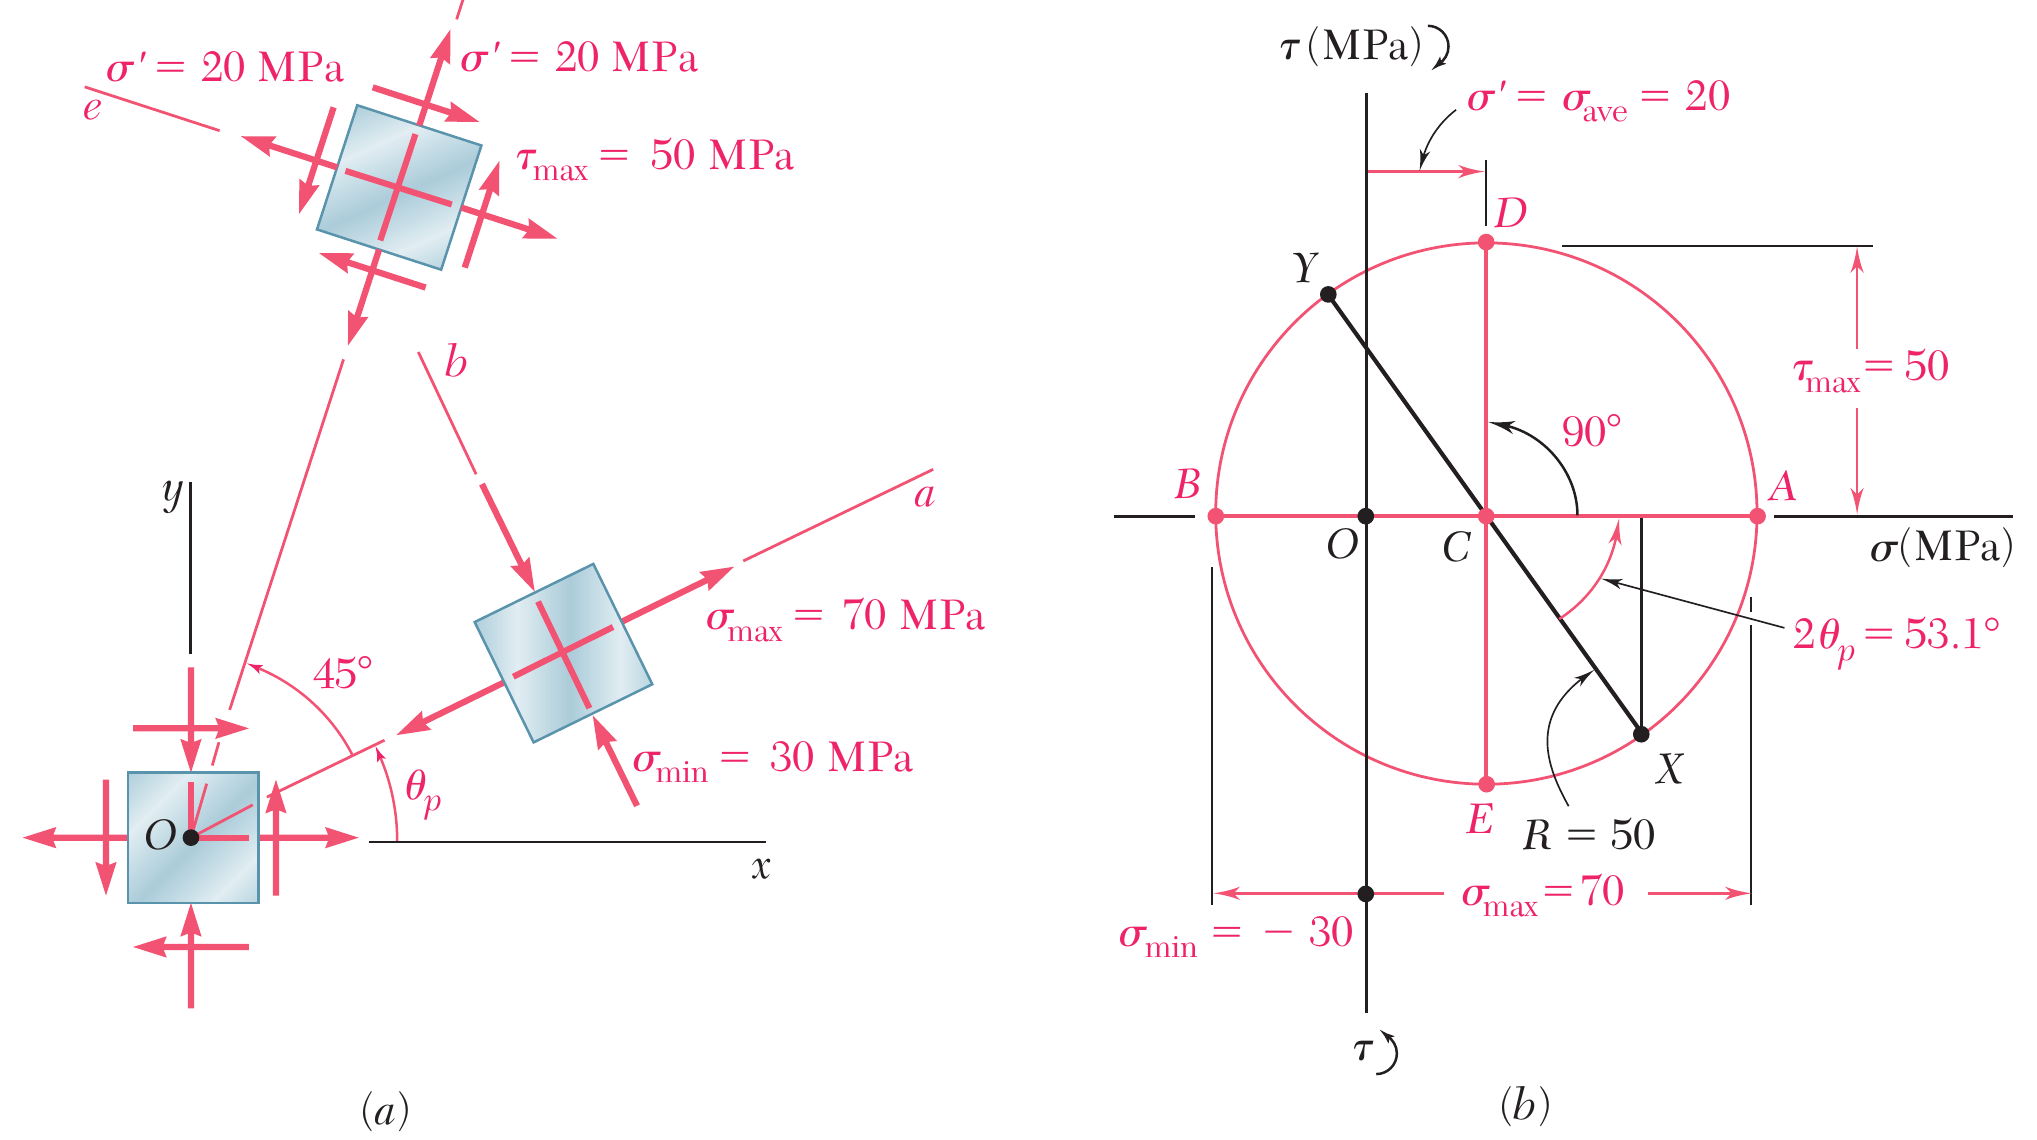
\includegraphics[width=\linewidth,height=2.6cm,keepaspectratio]{Chap_7/fig_7_20.png}
    \column{0.58\textwidth}
      \small
      Với trạng thái ứng suất phẳng như hình vẽ, (a) dựng vòng tròn Mohr,
      xác định (b) các mặt chính, (c) các ứng suất chính, (d) ứng suất tiếp
      lớn nhất và ứng suất pháp tương ứng.

      \vspace{0.5em}
      \textbf{LỜI GIẢI:}
      \begin{itemize}
        \item Dựng vòng tròn Mohr:
      \end{itemize}
      \[
        \sigma_{\mathrm{tb}} = \frac{\sigma_x + \sigma_y}{2}
          = \frac{(50) + (-10)}{2} = 20\,\mathrm{MPa}
      \]
      \[
        CF = 50 - 20 = 30\,\mathrm{MPa} \qquad FX = 40\,\mathrm{MPa}
      \]
      \[
        R = CX = \sqrt{(30)^2 + (40)^2} = 50\,\mathrm{MPa}
      \]
  \end{columns}
\end{frame}
% ===========
\begin{frame}[t]{Ví dụ 7.02 (tiếp)}
  \begin{columns}[T]
    \column{0.50\textwidth}
      \small
      \begin{itemize}
        \setlength{\itemsep}{0.5em}
        \item Các mặt chính và ứng suất chính:
        \[
          \tan2\theta_p = \frac{FX}{CF} = \frac{40}{30}
          \qquad 2\theta_p = 53{,}1^\circ
        \]
        \[
          \boxed{\theta_p = 26{,}6^\circ}
        \]
        \[
          \sigma_{\max} = OA = OC + CA = 20 + 50
        \]
        \[
          \boxed{\sigma_{\max} = 70\,\mathrm{MPa}}
        \]
        \[
          \sigma_{\min} = OB = OC - BC = 20 - 50
        \]
        \[
          \boxed{\sigma_{\min} = -30\,\mathrm{MPa}}
        \]
      \end{itemize}
    \column{0.48\textwidth}
      \centering
      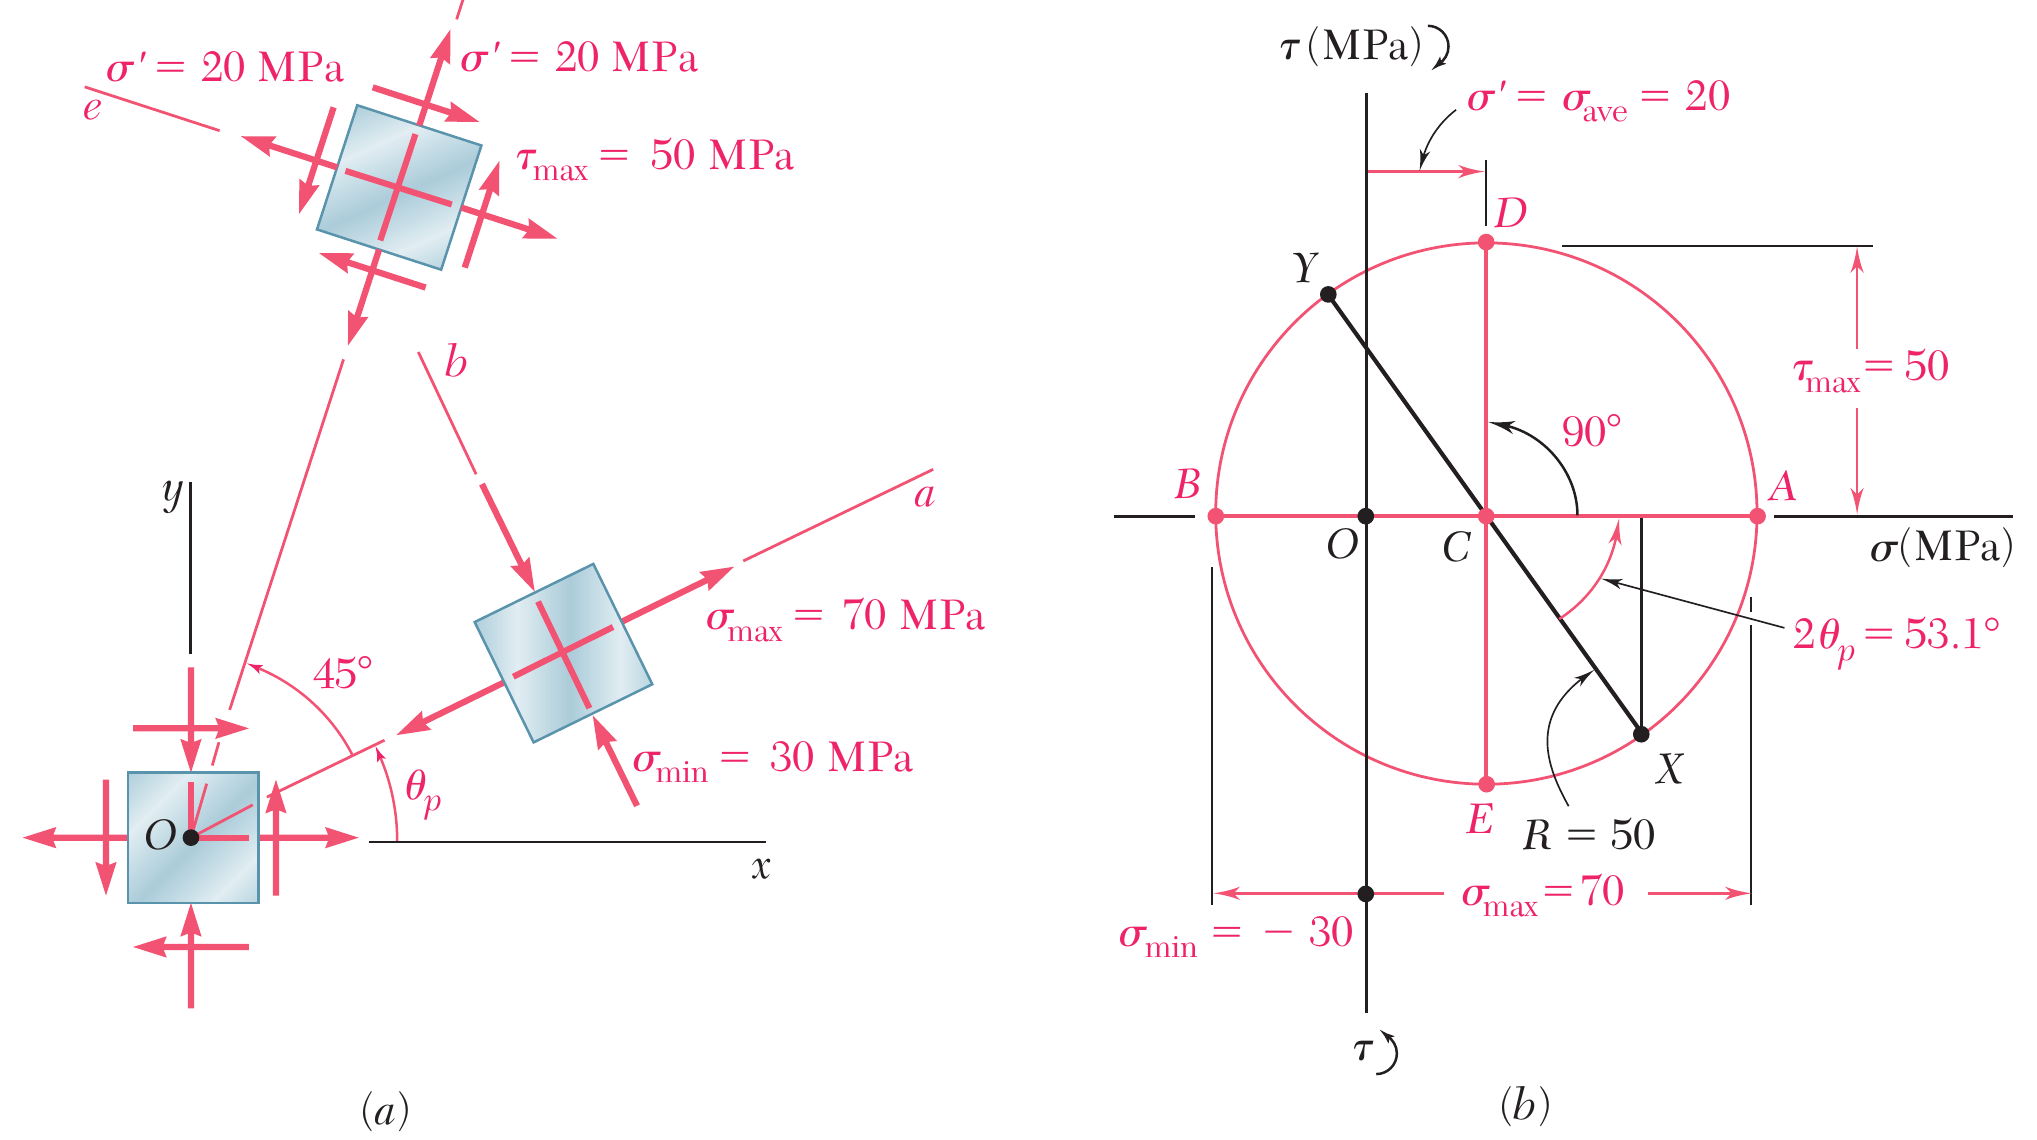
\includegraphics[width=\linewidth,height=5.5cm,keepaspectratio]{Chap_7/fig_7_20.png}
  \end{columns}
\end{frame}
% ===========
\begin{frame}[t]{Ví dụ 7.02 (tiếp)}
  \begin{columns}[T]
    \column{0.40\textwidth}
      \small
      \begin{itemize}
        \setlength{\itemsep}{0.5em}
        \item Ứng suất tiếp lớn nhất:
        \[
          \theta_s = \theta_p + 45^\circ
          \qquad \boxed{\theta_s = 71{,}6^\circ}
        \]
        \[
          \tau_{\max} = R
          \qquad \boxed{\tau_{\max} = 50\,\mathrm{MPa}}
        \]
        \[
          \sigma' = \sigma_{\mathrm{tb}}
          \qquad \boxed{\sigma' = 20\,\mathrm{MPa}}
        \]
      \end{itemize}
    \column{0.58\textwidth}
      \centering
      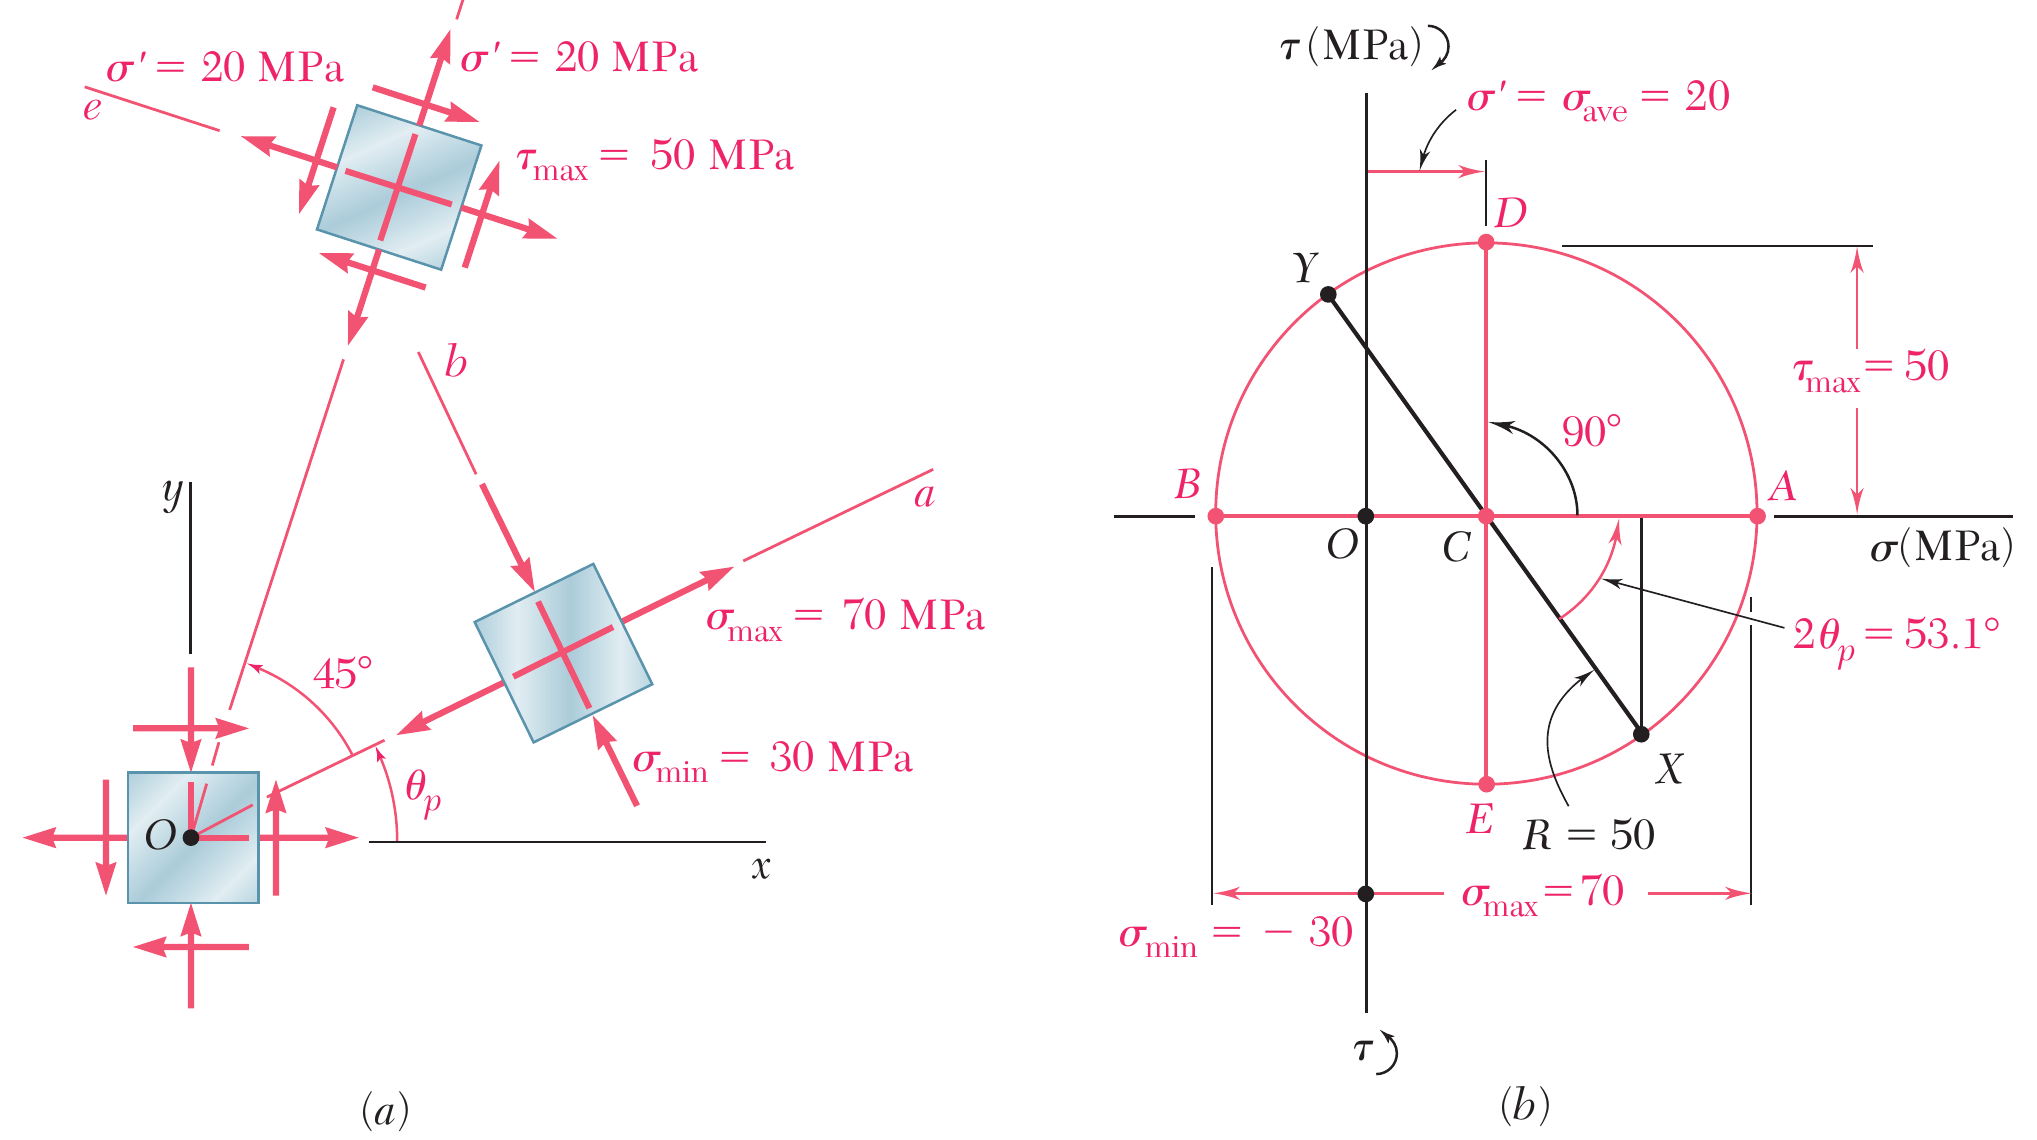
\includegraphics[width=0.49\linewidth,height=5.5cm,keepaspectratio]{Chap_7/fig_7_20.png}\hfill
      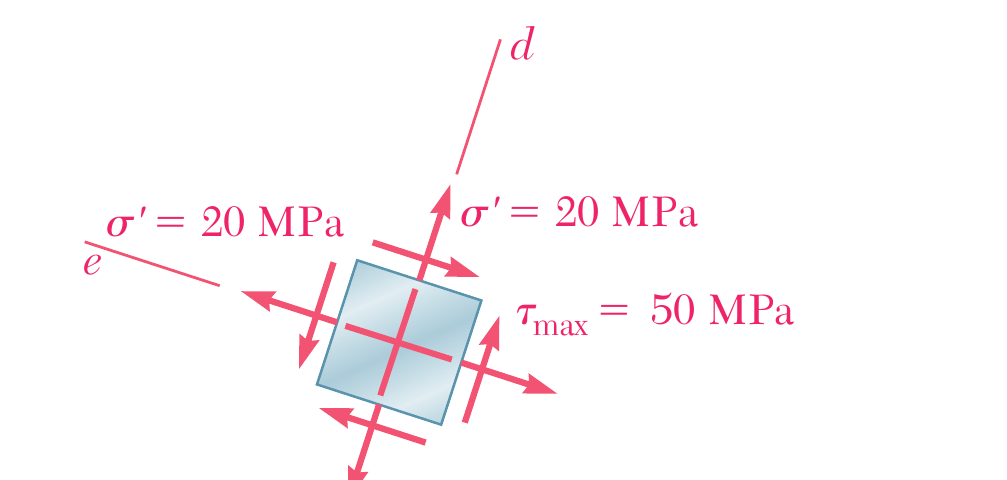
\includegraphics[width=0.49\linewidth,height=5.5cm,keepaspectratio]{Chap_7/ex_7_02.png}
  \end{columns}
\end{frame}
% ===========
\section{Bài mẫu 7.2}
\begin{frame}[t]{Bài mẫu 7.2}
  \begin{columns}[T]
    \column{0.40\textwidth}
      \centering
      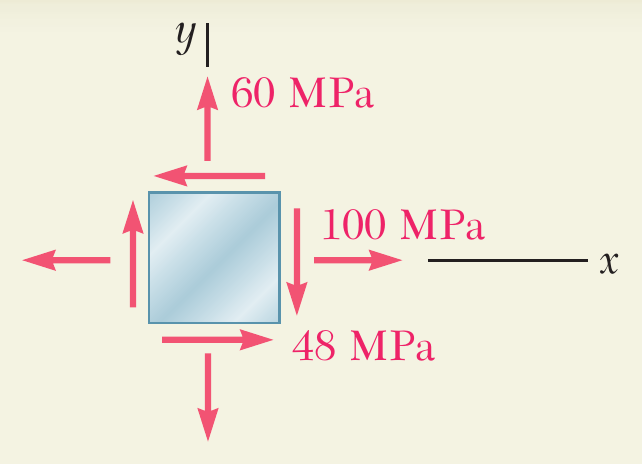
\includegraphics[width=\linewidth,height=2.9cm,keepaspectratio]{Chap_7/sp_7_2_a.png}\\[2pt]
      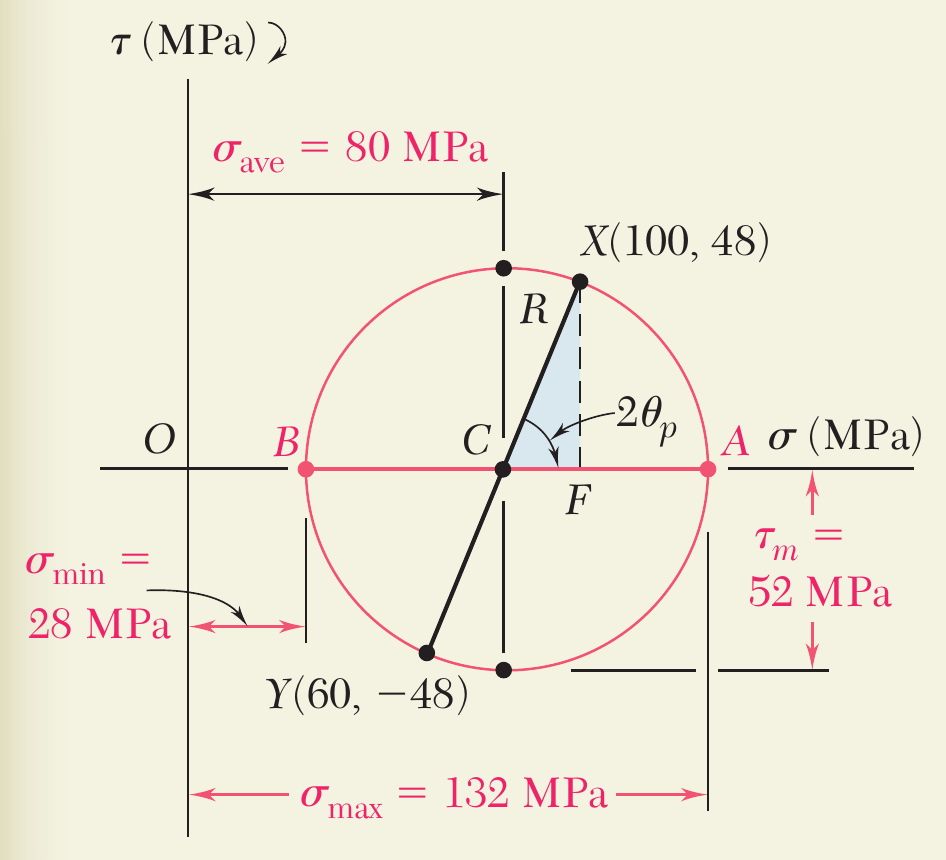
\includegraphics[width=\linewidth,height=2.9cm,keepaspectratio]{Chap_7/sp_7_2_b.png}
    \column{0.58\textwidth}
      \small
      Với trạng thái ứng suất như hình vẽ, xác định (a) các mặt chính và các
      ứng suất chính, (b) các thành phần ứng suất tác dụng lên phân tố nhận
      được bằng cách xoay phân tố đã cho ngược chiều kim đồng hồ một góc
      $30^\circ$.

      \vspace{0.5em}
      \textbf{LỜI GIẢI:}
      \begin{itemize}
        \item Dựng vòng tròn Mohr:
      \end{itemize}
      \[
        \sigma_{\mathrm{tb}} = \frac{\sigma_x + \sigma_y}{2}
          = \frac{100 + 60}{2} = 80\,\mathrm{MPa}
      \]
      \[
        R = \sqrt{(CF)^2 + (FX)^2} = \sqrt{(20)^2 + (48)^2} = 52\,\mathrm{MPa}
      \]
  \end{columns}
\end{frame}
% ===========
\begin{frame}[t]{Bài mẫu 7.2 (tiếp)}
  \begin{columns}[T]
    \column{0.48\textwidth}
      \small
      \begin{itemize}
        \setlength{\itemsep}{0.5em}
        \item Các mặt chính và ứng suất chính:
        \[
          \tan2\theta_p = \frac{XF}{CF} = \frac{48}{20} = 2{,}4
        \]
        \[
          2\theta_p = 67{,}4^\circ
        \]
        \[
          \boxed{\theta_p = 33{,}7^\circ \text{ cùng chiều kim đồng hồ}}
        \]
        \[
          \sigma_{\max} = OA = OC + CA = 80 + 52
        \]
        \[
          \boxed{\sigma_{\max} = +132\,\mathrm{MPa}}
        \]
        \[
          \sigma_{\min} = OB = OC - BC = 80 - 52
        \]
        \[
          \boxed{\sigma_{\min} = +28\,\mathrm{MPa}}
        \]
      \end{itemize}
    \column{0.50\textwidth}
      \centering
      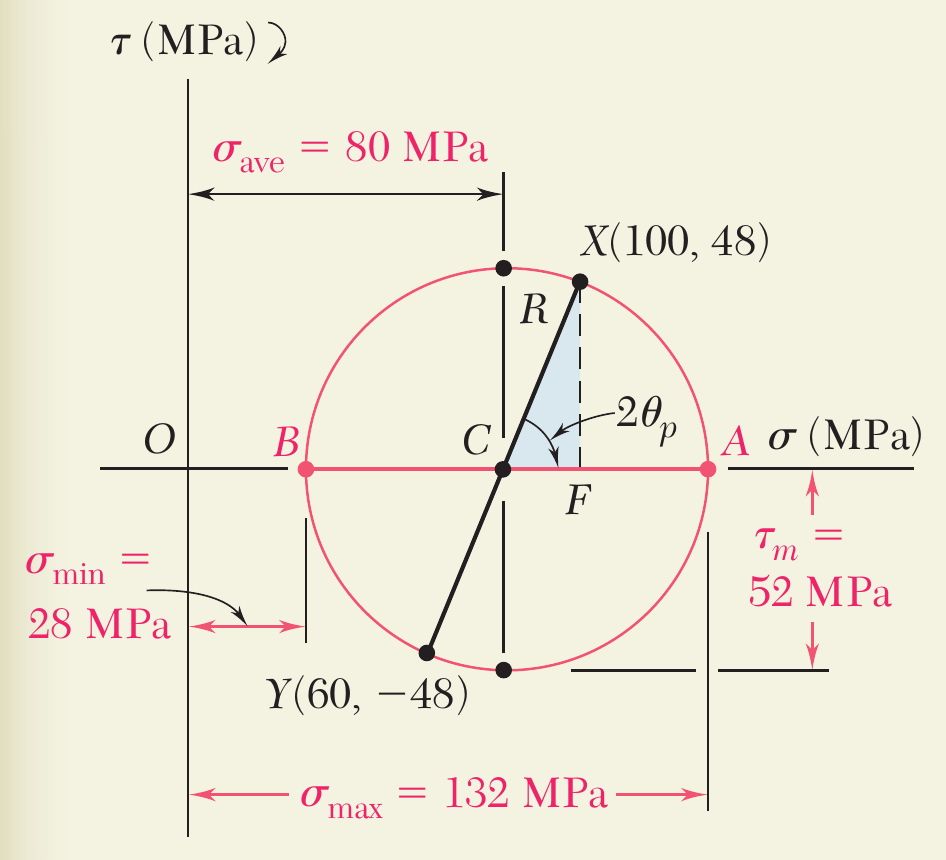
\includegraphics[width=\linewidth,height=2.9cm,keepaspectratio]{Chap_7/sp_7_2_b.png}\\[2pt]
      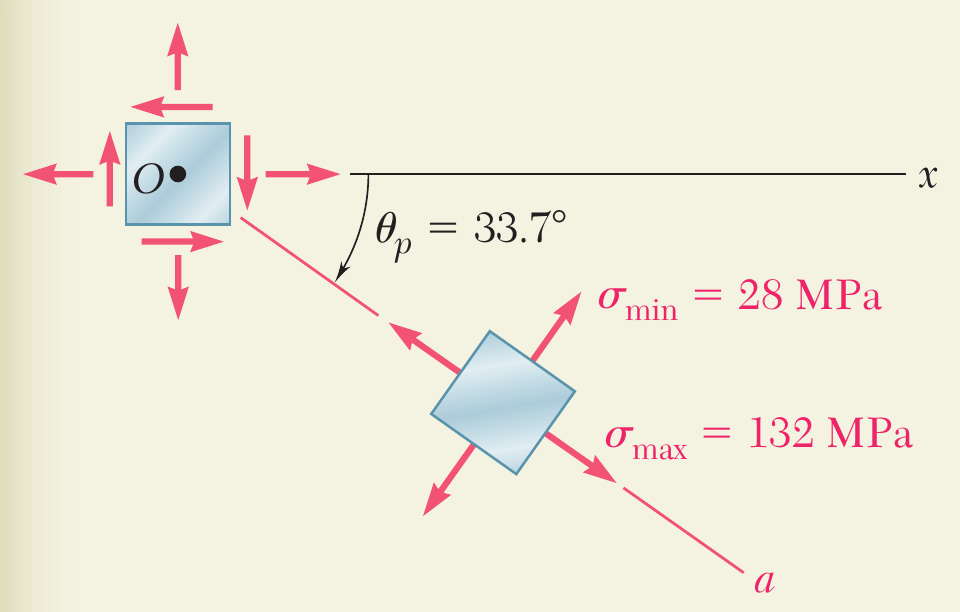
\includegraphics[width=\linewidth,height=2.9cm,keepaspectratio]{Chap_7/sp_7_2_c.png}
  \end{columns}
\end{frame}
% ===========
\begin{frame}[t]{Bài mẫu 7.2 (tiếp)}
  \begin{columns}[T]
    \column{0.52\textwidth}
      \small
      \begin{itemize}
        \setlength{\itemsep}{0.4em}
        \item Các thành phần ứng suất sau khi xoay $30^\circ$:

              Các điểm $X'$ và $Y'$ trên vòng tròn Mohr ứng với các thành
              phần ứng suất trên phân tố đã xoay nhận được bằng cách xoay $XY$
              ngược chiều kim đồng hồ một góc $2\theta = 60^\circ$.
        \[
          \phi = 180^\circ - 60^\circ - 67{,}4^\circ = 52{,}6^\circ
        \]
        \[
          \sigma_{x'} = OK = OC - KC = 80 - 52\cos52{,}6^\circ
        \]
        \[
          \sigma_{y'} = OL = OC + CL = 80 + 52\cos52{,}6^\circ
        \]
        \[
          \tau_{x'y'} = KX' = 52\sin52{,}6^\circ
        \]
        \[
          \boxed{\sigma_{x'} = +48{,}4\,\mathrm{MPa}} \quad
          \boxed{\sigma_{y'} = +111{,}6\,\mathrm{MPa}}
        \]
        \[
          \boxed{\tau_{x'y'} = 41{,}3\,\mathrm{MPa}}
        \]
      \end{itemize}
    \column{0.46\textwidth}
      \centering
      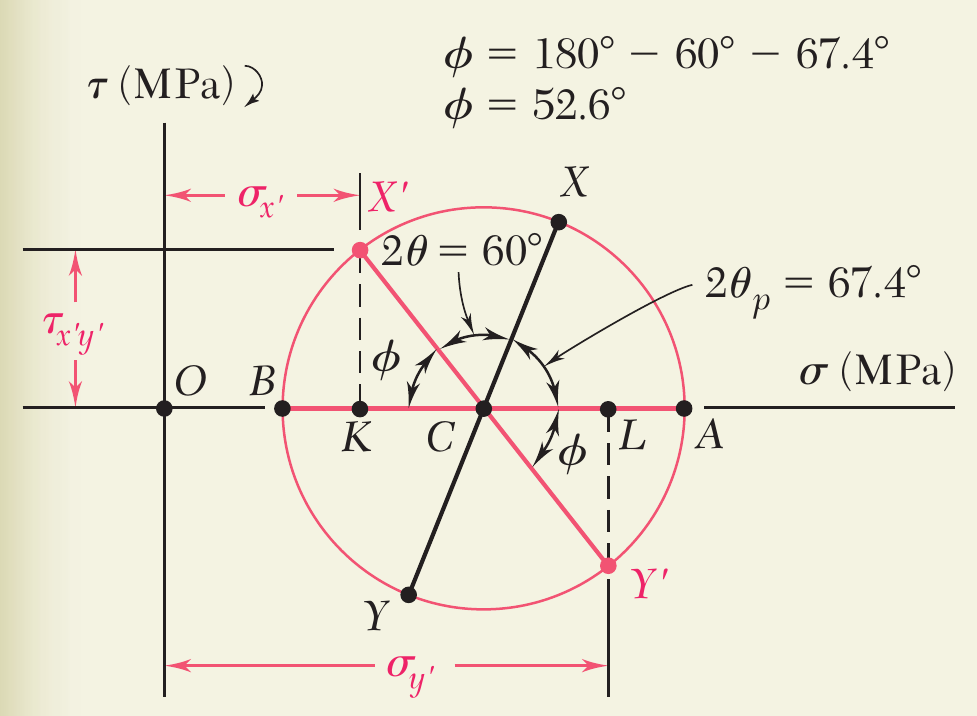
\includegraphics[width=\linewidth,height=2.9cm,keepaspectratio]{Chap_7/sp_7_2_d.png}\\[2pt]
      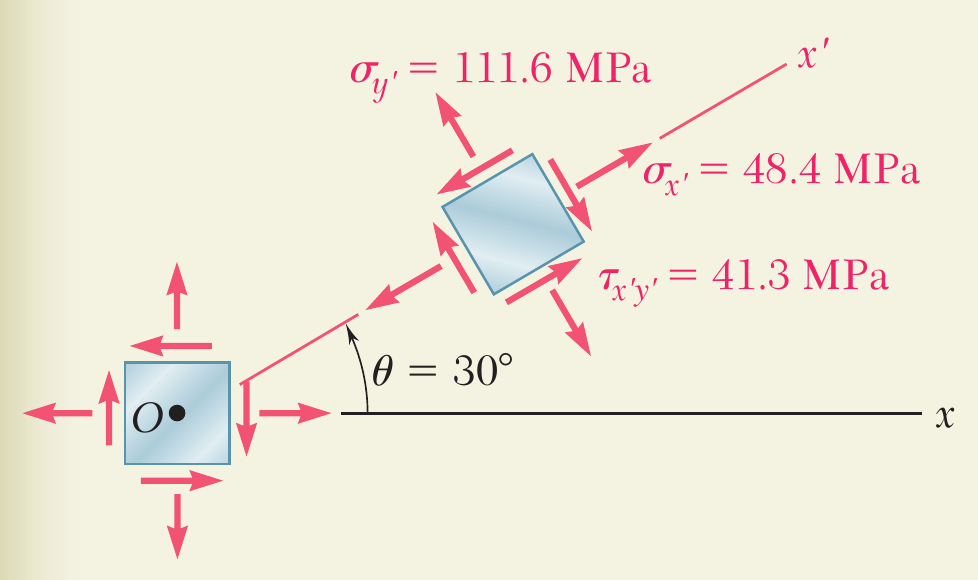
\includegraphics[width=\linewidth,height=2.9cm,keepaspectratio]{Chap_7/sp_7_2_e.png}
  \end{columns}
\end{frame}
% ===========
\section{Trạng thái ứng suất tổng quát}
\begin{frame}[t]{Trạng thái ứng suất tổng quát}
  \begin{columns}[T]
    \column{0.62\textwidth}
      \small
      \begin{itemize}
        \setlength{\itemsep}{0.3em}
        \item Xét trạng thái ứng suất 3D tổng quát tại một điểm và sự biến
              đổi ứng suất khi xoay phân tố.
        \item Trạng thái ứng suất tại $Q$ được xác định bởi:
              $\sigma_x, \sigma_y, \sigma_z, \tau_{xy}, \tau_{yz}, \tau_{zx}$
        \item Xét tứ diện có một mặt vuông góc với đường $QN$ với các cô sin
              chỉ phương: $\lambda_x, \lambda_y, \lambda_z$
        \item Điều kiện $\sum F_n = 0$ dẫn tới:
        \[
          \sigma_n = \sigma_x\lambda_x^2 + \sigma_y\lambda_y^2 + \sigma_z\lambda_z^2
            + 2\tau_{xy}\lambda_x\lambda_y + 2\tau_{yz}\lambda_y\lambda_z
            + 2\tau_{zx}\lambda_z\lambda_x
        \]
        \item Dạng của phương trình đảm bảo rằng có thể tìm được một hướng
              phân tố sao cho:
        \[
          \sigma_n = \sigma_a\lambda_a^2 + \sigma_b\lambda_b^2 + \sigma_c\lambda_c^2
        \]
        Đây là các trục chính và mặt chính, và các ứng suất pháp là các ứng
        suất chính.
      \end{itemize}
    \column{0.36\textwidth}
      \centering
      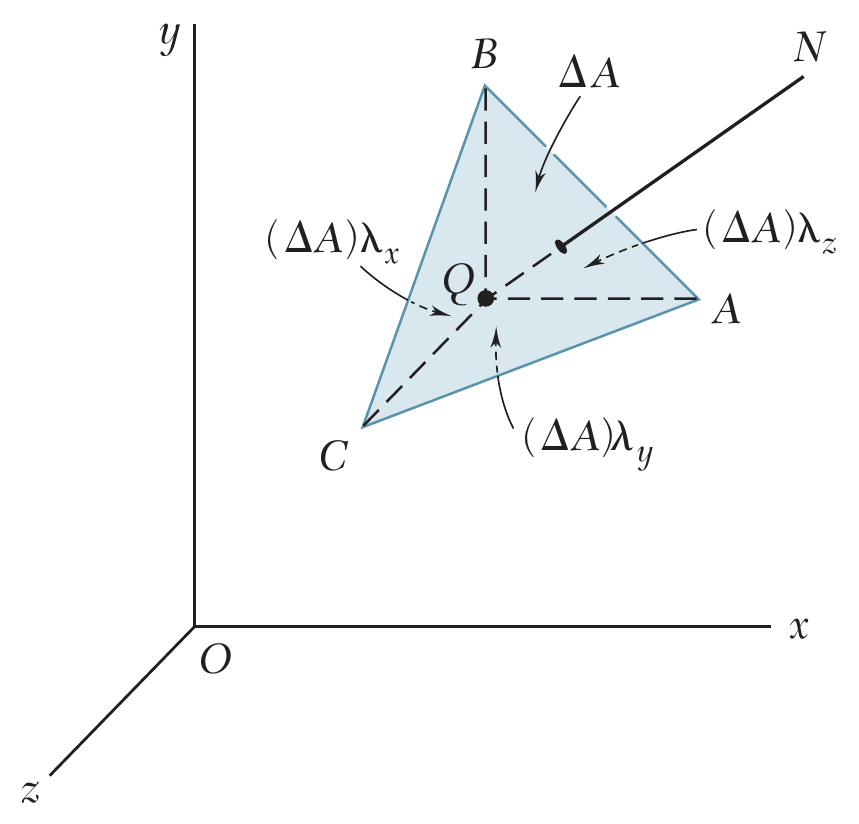
\includegraphics[width=\linewidth,height=2.9cm,keepaspectratio]{Chap_7/fig_7_23.png}\\[2pt]
      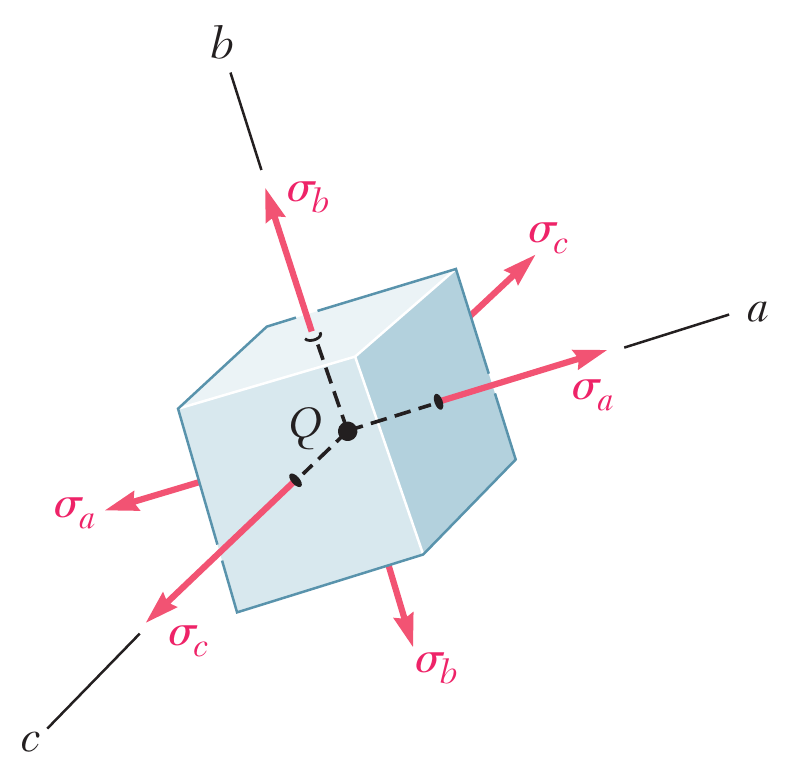
\includegraphics[width=\linewidth,height=2.9cm,keepaspectratio]{Chap_7/fig_7_25.png}
  \end{columns}
\end{frame}
% ===========
\section{Vòng tròn Mohr trong phân tích ứng suất ba chiều}
\begin{frame}[t]{Ứng dụng vòng tròn Mohr trong phân tích ứng suất ba chiều}
  \begin{columns}[T]
    \column{0.58\textwidth}
      \small
      \begin{itemize}
        \setlength{\itemsep}{0.5em}
        \item Sự biến đổi ứng suất của phân tố xoay quanh một trục chính có
              thể được biểu diễn bằng vòng tròn Mohr.
        \item Các điểm $A$, $B$ và $C$ biểu diễn các ứng suất chính trên các
              mặt chính (ứng suất tiếp bằng không).
        \item Ba vòng tròn biểu diễn ứng suất pháp và ứng suất tiếp khi xoay
              quanh từng trục chính.
        \item Bán kính của vòng tròn lớn nhất cho ứng suất tiếp lớn nhất:
        \[
          \tau_{\max} = \tfrac{1}{2}\left|\sigma_{\max} - \sigma_{\min}\right|
        \]
      \end{itemize}
    \column{0.40\textwidth}
      \centering
      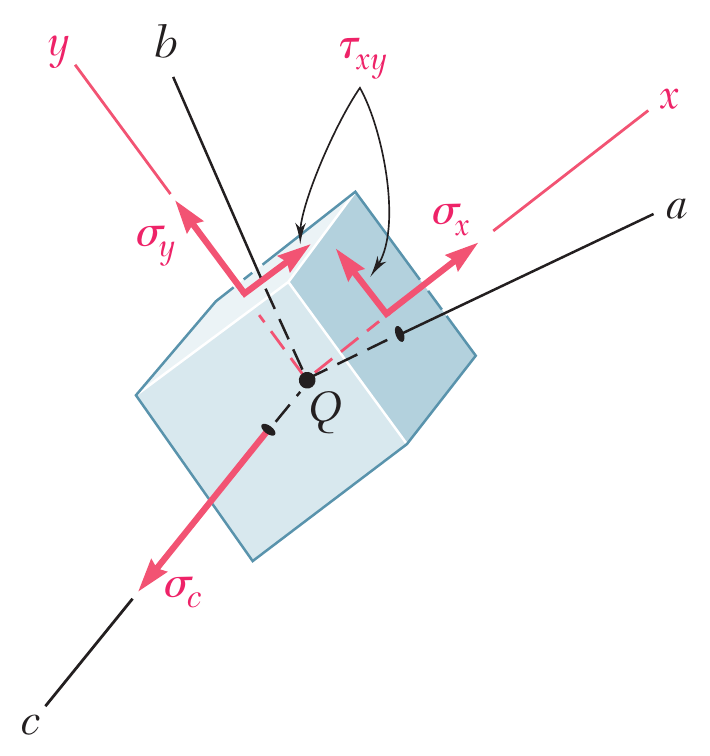
\includegraphics[width=\linewidth,height=2.9cm,keepaspectratio]{Chap_7/fig_7_26.png}\\[2pt]
      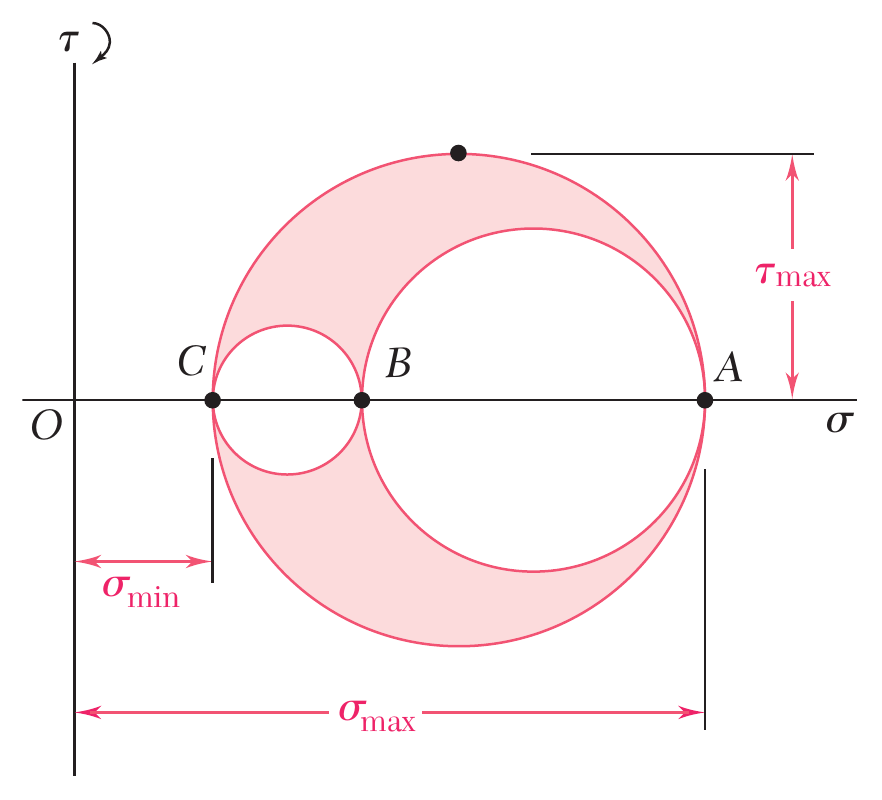
\includegraphics[width=\linewidth,height=2.9cm,keepaspectratio]{Chap_7/fig_7_27.png}
  \end{columns}
\end{frame}
% ===========
\begin{frame}[t]{Ứng dụng vòng tròn Mohr trong phân tích ứng suất ba chiều (tiếp)}
  \begin{columns}[T]
    \column{0.58\textwidth}
      \small
      \begin{itemize}
        \setlength{\itemsep}{0.5em}
        \item Trong trường hợp ứng suất phẳng, trục vuông góc với mặt phẳng
              ứng suất là một trục chính (ứng suất tiếp bằng không).
        \item Nếu các điểm $A$ và $B$ (biểu diễn các mặt chính) nằm ở hai phía
              của gốc tọa độ thì:
              \begin{enumerate}[a)]
                \item các ứng suất chính tương ứng là ứng suất pháp lớn nhất
                      và nhỏ nhất của phân tố
                \item ứng suất tiếp lớn nhất của phân tố bằng ứng suất tiếp
                      lớn nhất ``trong mặt phẳng''
                \item các mặt có ứng suất tiếp lớn nhất nghiêng $45^\circ$ so
                      với các mặt chính.
              \end{enumerate}
      \end{itemize}
    \column{0.40\textwidth}
      \centering
      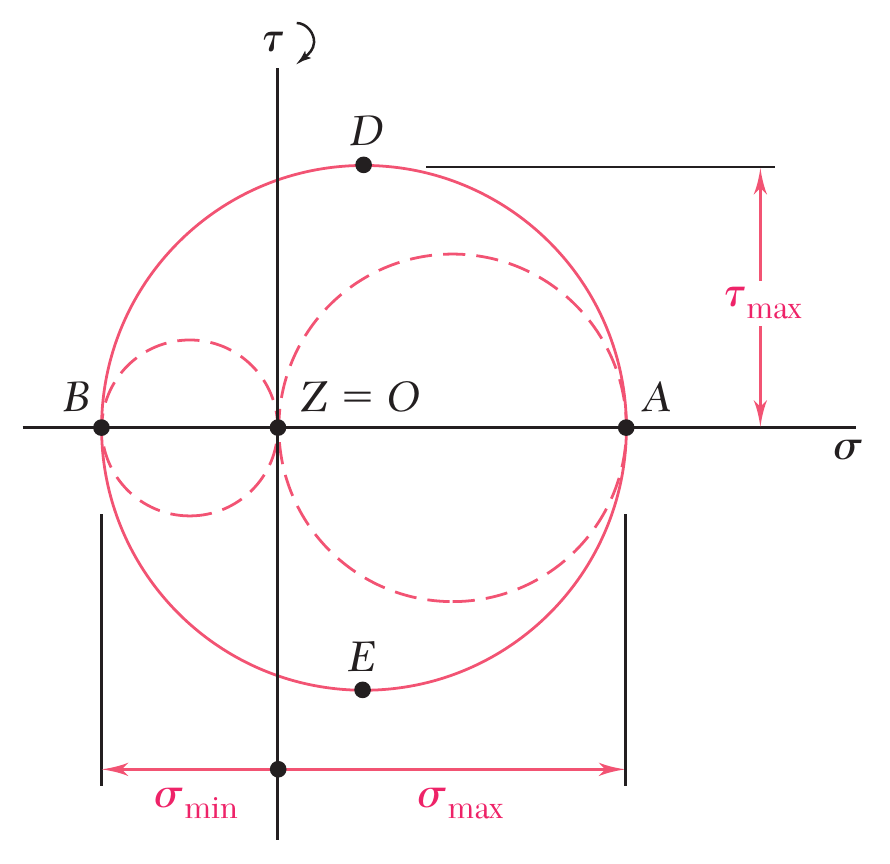
\includegraphics[width=\linewidth,height=2.9cm,keepaspectratio]{Chap_7/fig_7_28.png}\\[2pt]
      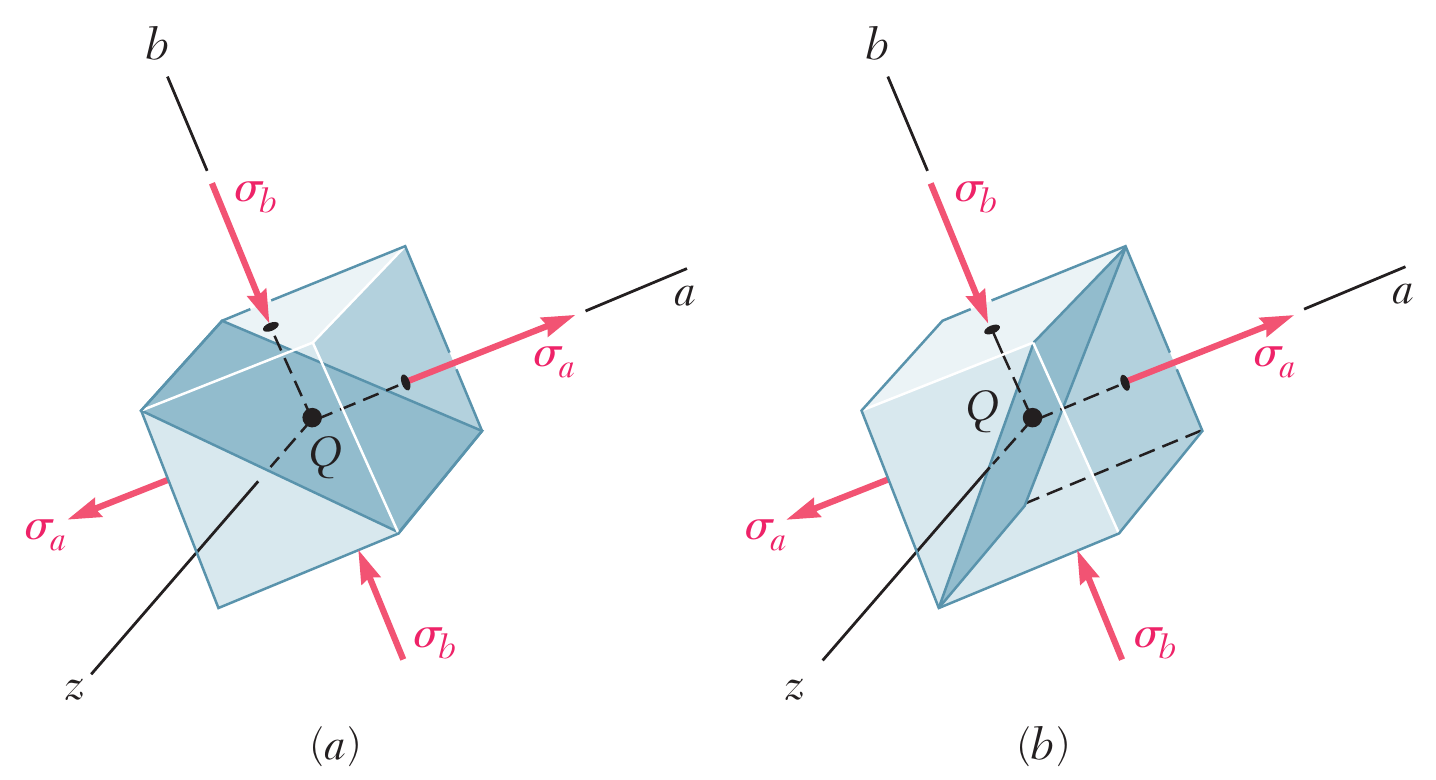
\includegraphics[width=\linewidth,height=2.9cm,keepaspectratio]{Chap_7/fig_7_29.png}
  \end{columns}
\end{frame}
% ===========
\begin{frame}[t]{Ứng dụng vòng tròn Mohr trong phân tích ứng suất ba chiều (tiếp)}
  \begin{columns}[T]
    \column{0.58\textwidth}
      \small
      \begin{itemize}
        \setlength{\itemsep}{0.5em}
        \item Nếu $A$ và $B$ nằm cùng phía với gốc tọa độ (tức là cùng dấu)
              thì:
              \begin{enumerate}[a)]
                \item vòng tròn xác định $\sigma_{\max}$, $\sigma_{\min}$ và
                      $\tau_{\max}$ của phân tố không phải là vòng tròn ứng với
                      các phép biến đổi trong mặt phẳng ứng suất
                \item ứng suất tiếp lớn nhất của phân tố bằng một nửa ứng
                      suất lớn nhất
                \item các mặt có ứng suất tiếp lớn nhất nghiêng $45^\circ$ so
                      với mặt phẳng ứng suất.
              \end{enumerate}
      \end{itemize}
    \column{0.40\textwidth}
      \centering
      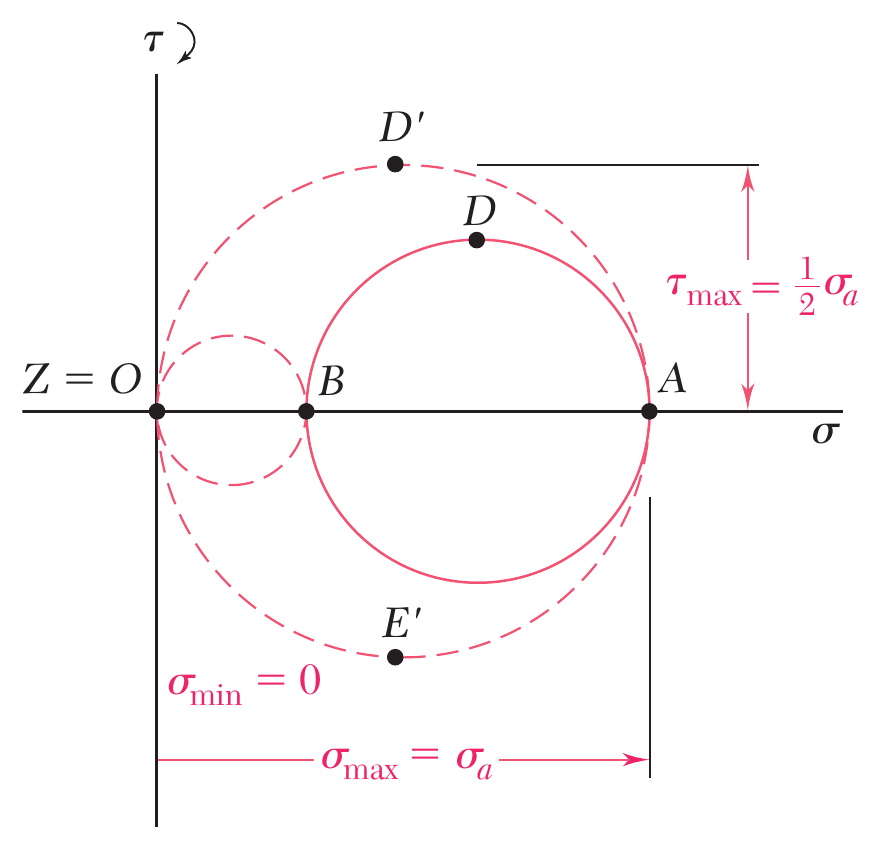
\includegraphics[width=\linewidth,height=5.5cm,keepaspectratio]{Chap_7/fig_7_30.png}
  \end{columns}
\end{frame}
% ===========
\section{Tiêu chuẩn chảy dẻo cho vật liệu dẻo}
\begin{frame}[t]{Tiêu chuẩn chảy dẻo cho vật liệu dẻo ở trạng thái ứng suất phẳng}
  \begin{columns}[T]
    \column{0.58\textwidth}
      \small
      \begin{itemize}
        \setlength{\itemsep}{0.5em}
        \item Sự phá hủy của chi tiết máy chịu ứng suất đơn trục được dự báo
              trực tiếp từ thí nghiệm kéo tương đương.
        \item Sự phá hủy của chi tiết máy chịu ứng suất phẳng không thể dự
              báo trực tiếp từ trạng thái ứng suất đơn trục của mẫu thử kéo.
        \item Thuận tiện là xác định các ứng suất chính và xây dựng tiêu chuẩn
              phá hủy dựa trên trạng thái ứng suất hai trục tương ứng.
        \item Tiêu chuẩn phá hủy dựa trên cơ chế phá hủy, cho phép so sánh
              điều kiện phá hủy giữa thí nghiệm ứng suất đơn trục và chi tiết
              chịu tải hai trục.
      \end{itemize}
    \column{0.40\textwidth}
      \centering
      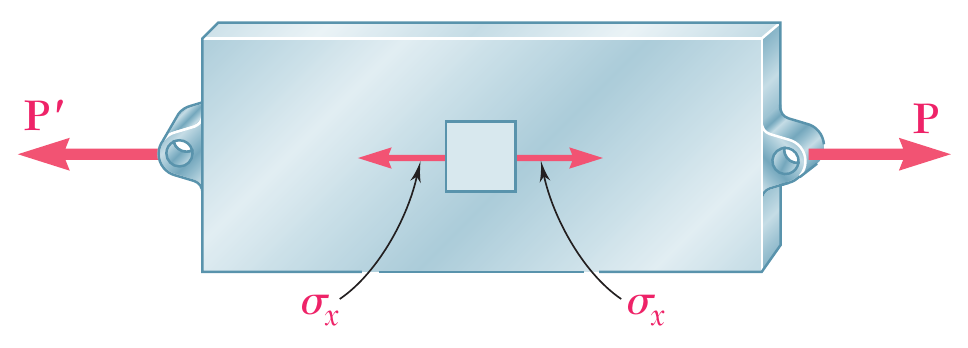
\includegraphics[width=\linewidth,height=2.9cm,keepaspectratio]{Chap_7/fig_7_36.png}\\[2pt]
      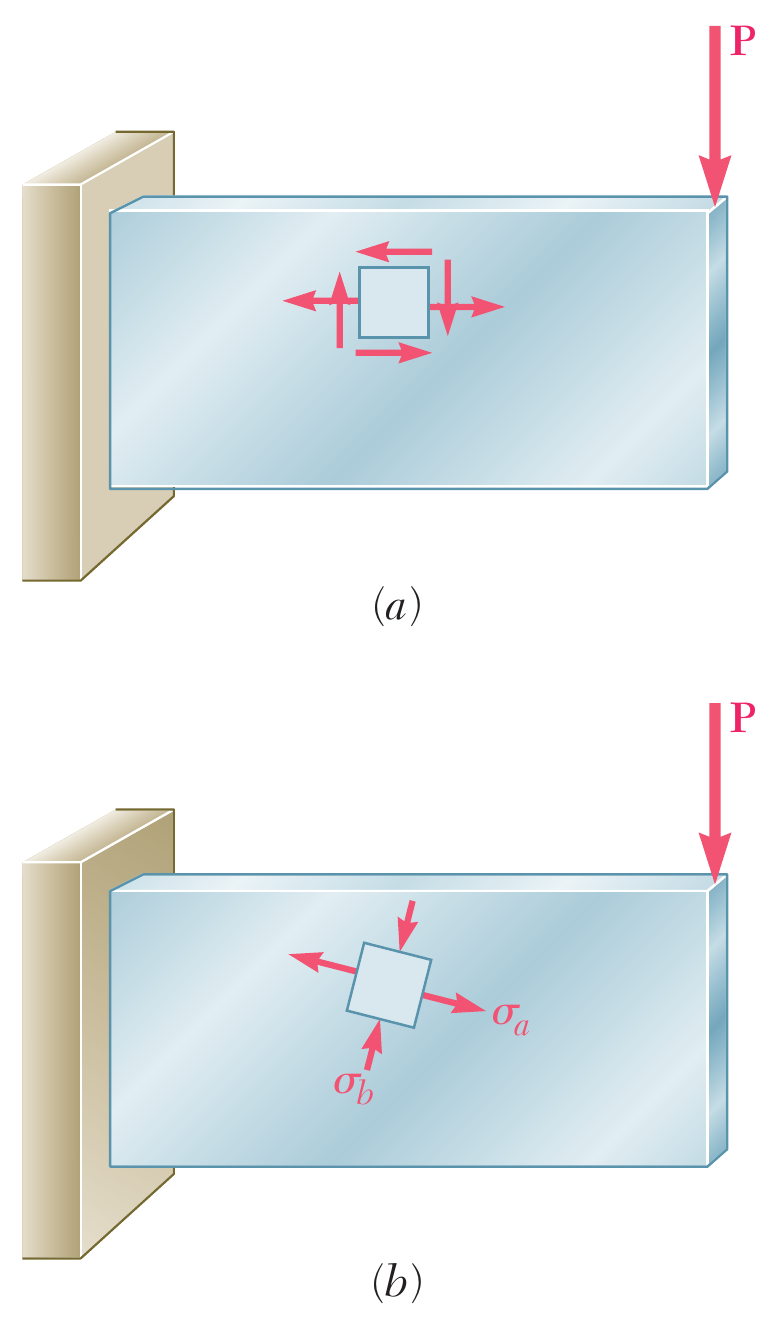
\includegraphics[width=\linewidth,height=2.9cm,keepaspectratio]{Chap_7/fig_7_37.png}
  \end{columns}
\end{frame}
% ===========
\begin{frame}[t]{Tiêu chuẩn chảy dẻo: ứng suất tiếp lớn nhất (Tresca)}
  \begin{columns}[T]
    \column{0.58\textwidth}
      \small
      \textbf{Tiêu chuẩn ứng suất tiếp lớn nhất:}

      Cấu kiện an toàn khi ứng suất tiếp lớn nhất còn nhỏ hơn ứng suất tiếp
      lớn nhất của mẫu thử kéo tại thời điểm chảy, tức là:
      \[
        \tau_{\max} < \tau_Y = \frac{\sigma_Y}{2}
      \]
      Với $\sigma_a$ và $\sigma_b$ cùng dấu:
      \[
        \tau_{\max} = \frac{|\sigma_a|}{2} \ \text{hoặc}\ \frac{|\sigma_b|}{2}
          < \frac{\sigma_Y}{2}
      \]
      Với $\sigma_a$ và $\sigma_b$ trái dấu:
      \[
        \tau_{\max} = \frac{|\sigma_a - \sigma_b|}{2} < \frac{\sigma_Y}{2}
      \]
    \column{0.40\textwidth}
      \centering
      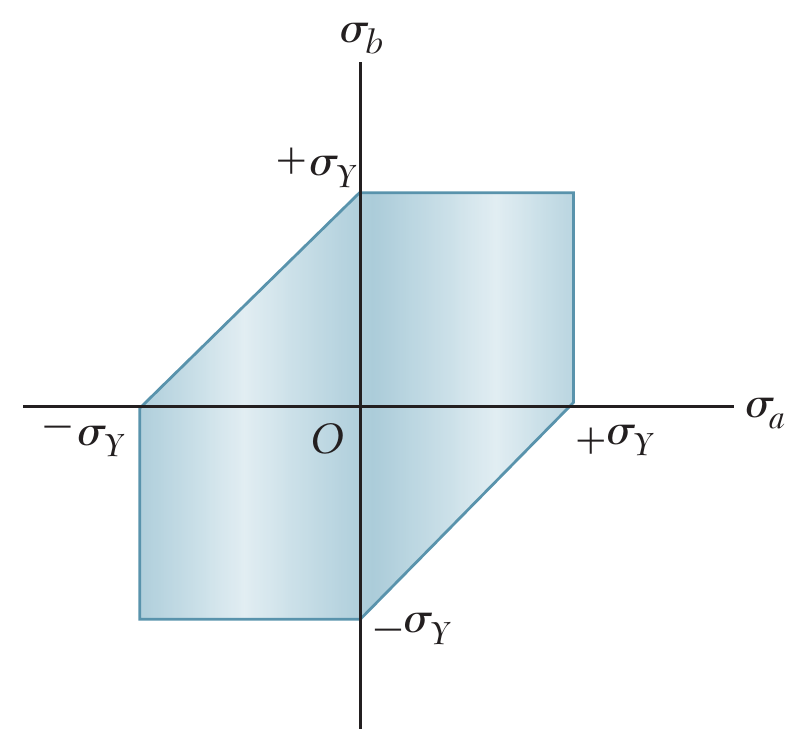
\includegraphics[width=\linewidth,height=5.5cm,keepaspectratio]{Chap_7/fig_7_38.png}
  \end{columns}
\end{frame}
% ===========
\begin{frame}[t]{Tiêu chuẩn chảy dẻo: năng lượng biến dạng hình dáng lớn nhất (von Mises)}
  \begin{columns}[T]
    \column{0.58\textwidth}
      \small
      \textbf{Tiêu chuẩn năng lượng biến dạng hình dáng lớn nhất:}

      Cấu kiện an toàn khi năng lượng biến dạng hình dáng trên một đơn vị
      thể tích còn nhỏ hơn giá trị đó của mẫu thử kéo tại thời điểm chảy.
      \[
        u_d < u_Y
      \]
      \[
        \frac{1}{6G}\left(\sigma_a^2 - \sigma_a\sigma_b + \sigma_b^2\right)
          < \frac{1}{6G}\left(\sigma_Y^2 - \sigma_Y\times0 + 0^2\right)
      \]
      \[
        \sigma_a^2 - \sigma_a\sigma_b + \sigma_b^2 < \sigma_Y^2
      \]
    \column{0.40\textwidth}
      \centering
      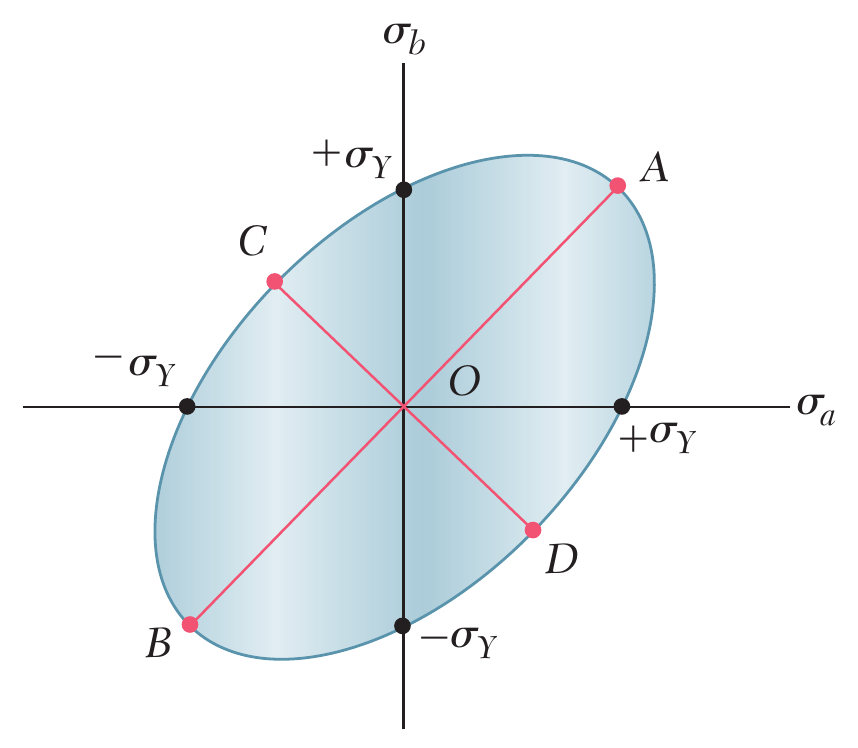
\includegraphics[width=\linewidth,height=5.5cm,keepaspectratio]{Chap_7/fig_7_39.png}
  \end{columns}
\end{frame}
% ===========
\section{Tiêu chuẩn phá hủy cho vật liệu giòn}
\begin{frame}[t]{Tiêu chuẩn phá hủy cho vật liệu giòn ở trạng thái ứng suất phẳng}
  \begin{columns}[T]
    \column{0.58\textwidth}
      \small
      Vật liệu giòn bị phá hủy đột ngột do đứt gãy trong thí nghiệm kéo. Điều
      kiện phá hủy được đặc trưng bởi giới hạn bền $\sigma_U$.

      \vspace{0.8em}
      \textbf{Tiêu chuẩn ứng suất pháp lớn nhất:}

      Cấu kiện an toàn khi ứng suất pháp lớn nhất còn nhỏ hơn giới hạn bền
      của mẫu thử kéo:
      \[
        |\sigma_a| < \sigma_U \qquad |\sigma_b| < \sigma_U
      \]
    \column{0.40\textwidth}
      \centering
      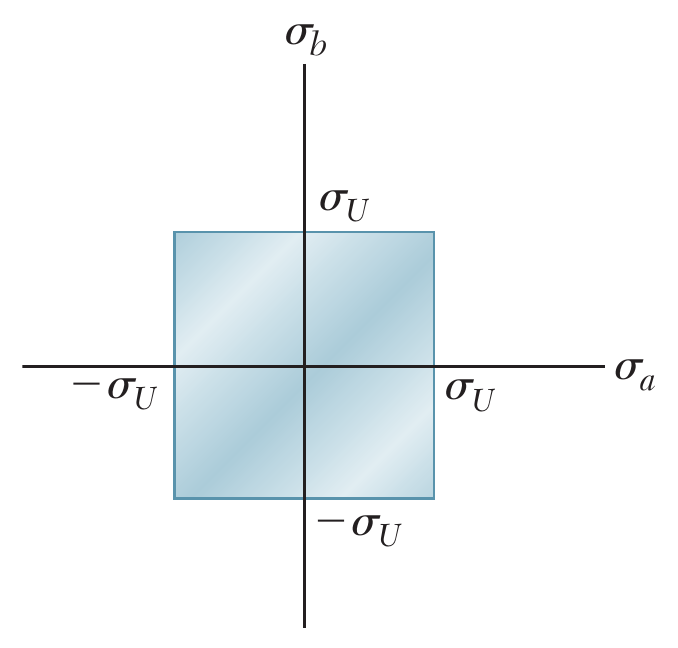
\includegraphics[width=\linewidth,height=5.5cm,keepaspectratio]{Chap_7/fig_7_41.png}
  \end{columns}
\end{frame}
% ===========
\section{Ứng suất trong bình chịu áp thành mỏng}
\begin{frame}[t]{Ứng suất trong bình chịu áp thành mỏng}
  \begin{columns}[T]
    \column{0.56\textwidth}
      \small
      \begin{itemize}
        \setlength{\itemsep}{0.5em}
        \item Bình hình trụ với các ứng suất chính:\\
              $\sigma_1$ = ứng suất vòng (ứng suất tiếp tuyến)\\
              $\sigma_2$ = ứng suất dọc
        \item Ứng suất vòng:
        \[
          \textstyle\sum F_z = 0 = \sigma_1(2t\Delta x) - p(2r\Delta x)
          \qquad \sigma_1 = \frac{pr}{t}
        \]
        \item Ứng suất dọc:
        \[
          \textstyle\sum F_x = 0 = \sigma_2(2\pi rt) - p(\pi r^2)
          \qquad \sigma_2 = \frac{pr}{2t}
        \]
        \[
          \sigma_1 = 2\sigma_2
        \]
      \end{itemize}
    \column{0.42\textwidth}
      \centering
      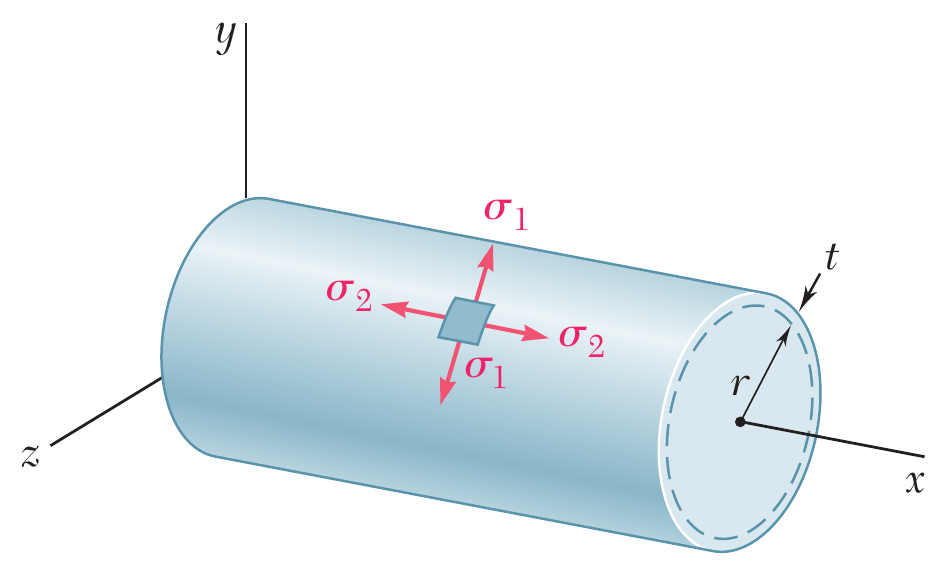
\includegraphics[width=\linewidth,height=2.9cm,keepaspectratio]{Chap_7/fig_7_47.png}\\[2pt]
      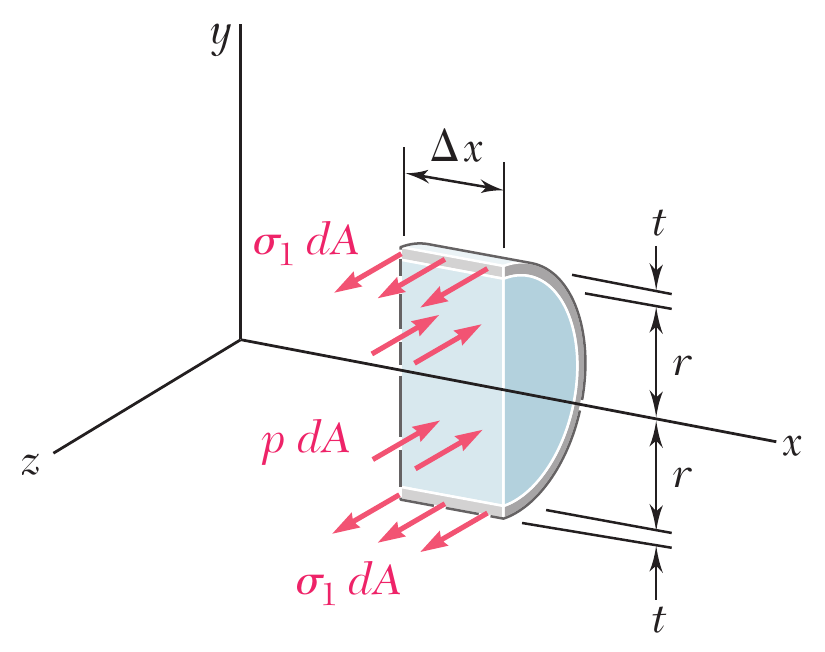
\includegraphics[width=\linewidth,height=2.9cm,keepaspectratio]{Chap_7/fig_7_48.png}
  \end{columns}
\end{frame}
% ===========
\begin{frame}[t]{Ứng suất trong bình chịu áp thành mỏng (tiếp)}
  \begin{columns}[T]
    \column{0.58\textwidth}
      \small
      \begin{itemize}
        \setlength{\itemsep}{0.6em}
        \item Các điểm $A$ và $B$ ứng với ứng suất vòng $\sigma_1$ và ứng
              suất dọc $\sigma_2$.
        \item Ứng suất tiếp lớn nhất trong mặt phẳng:
        \[
          \tau_{\max(\text{trong mặt phẳng})} = \tfrac{1}{2}\sigma_2 = \frac{pr}{4t}
        \]
        \item Ứng suất tiếp lớn nhất ngoài mặt phẳng ứng với phép xoay
              $45^\circ$ của phân tố ứng suất phẳng quanh trục dọc:
        \[
          \tau_{\max} = \sigma_2 = \frac{pr}{2t}
        \]
      \end{itemize}
    \column{0.40\textwidth}
      \centering
      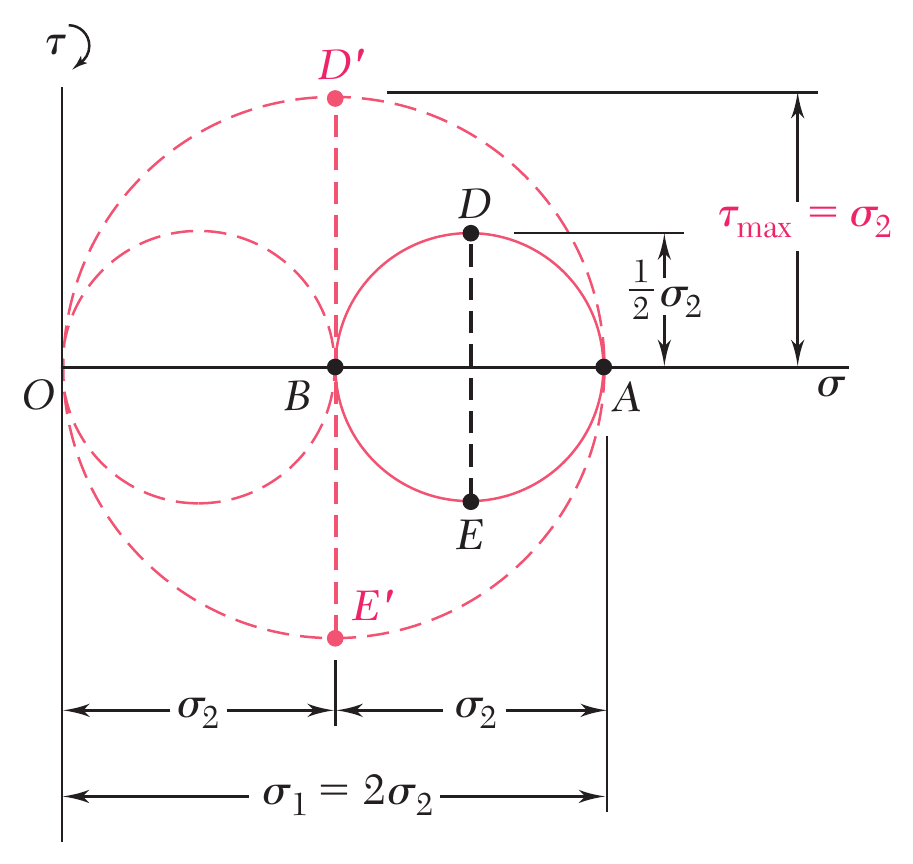
\includegraphics[width=\linewidth,height=5.5cm,keepaspectratio]{Chap_7/fig_7_50.png}
  \end{columns}
\end{frame}
% ===========
\begin{frame}[t]{Ứng suất trong bình chịu áp thành mỏng (tiếp)}
  \begin{columns}[T]
    \column{0.58\textwidth}
      \small
      \begin{itemize}
        \setlength{\itemsep}{0.6em}
        \item Bình chịu áp hình cầu:
        \[
          \sigma_1 = \sigma_2 = \frac{pr}{2t}
        \]
        \item Vòng tròn Mohr cho các phép biến đổi trong mặt phẳng suy biến
              thành một điểm:
        \[
          \sigma = \sigma_1 = \sigma_2 = \text{const} \qquad
          \tau_{\max(\text{trong mặt phẳng})} = 0
        \]
        \item Ứng suất tiếp lớn nhất ngoài mặt phẳng:
        \[
          \tau_{\max} = \tfrac{1}{2}\sigma_1 = \frac{pr}{4t}
        \]
      \end{itemize}
    \column{0.40\textwidth}
      \centering
      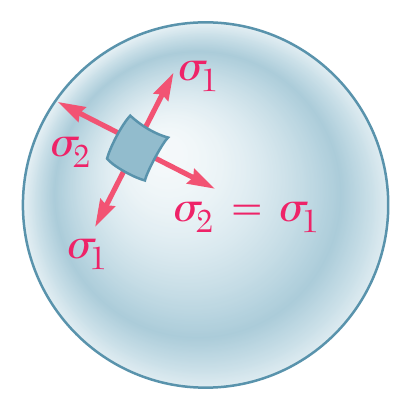
\includegraphics[width=\linewidth,height=1.9cm,keepaspectratio]{Chap_7/fig_7_51.png}\\[2pt]
      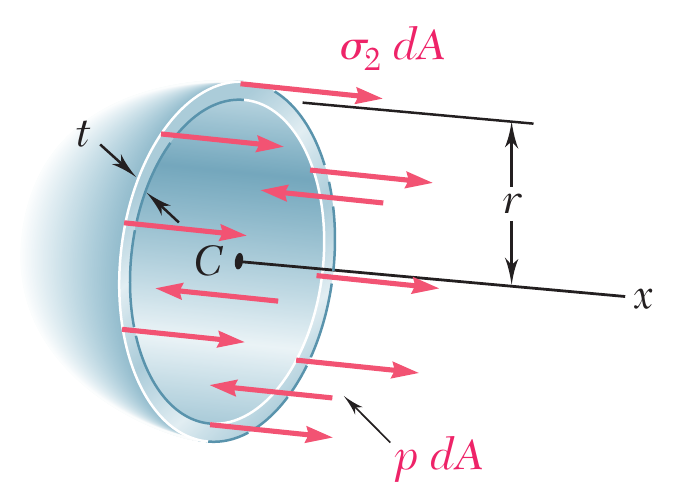
\includegraphics[width=\linewidth,height=1.9cm,keepaspectratio]{Chap_7/fig_7_52.png}\\[2pt]
      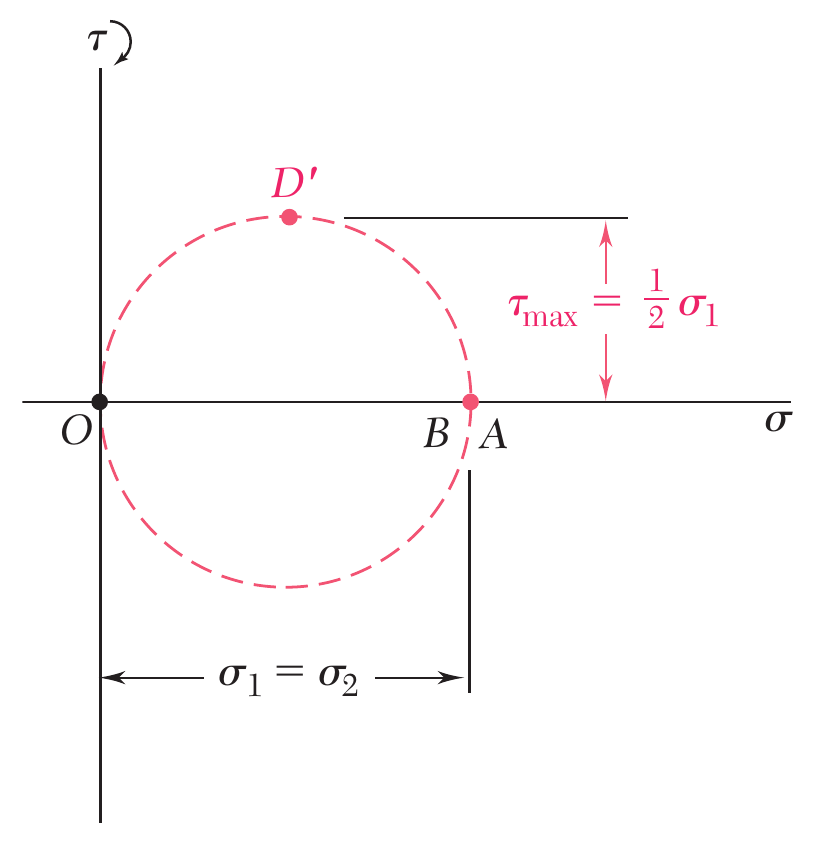
\includegraphics[width=\linewidth,height=1.9cm,keepaspectratio]{Chap_7/fig_7_53.png}
  \end{columns}
\end{frame}
% ===========
\section{Biến đổi biến dạng phẳng}
\begin{frame}[t]{Biến đổi biến dạng phẳng}
  \begin{columns}[T]
    \column{0.58\textwidth}
      \small
      \begin{itemize}
        \setlength{\itemsep}{0.4em}
        \item \textbf{Biến dạng phẳng} -- biến dạng của vật liệu xảy ra trong
              các mặt phẳng song song và như nhau trong mỗi mặt phẳng đó.
        \item Biến dạng phẳng xảy ra trong tấm chịu tải trọng phân bố đều dọc
              theo các mép và bị ngăn cản giãn nở hoặc co ngang bởi các gối
              cứng, nhẵn và cố định.

              Các thành phần biến dạng:
              \[
                \varepsilon_x\ \ \varepsilon_y\ \ \gamma_{xy}
                \quad (\varepsilon_z = \gamma_{zx} = \gamma_{zy} = 0)
              \]
        \item Ví dụ: xét một thanh dài chịu tải trọng ngang phân bố đều.
              Trạng thái biến dạng phẳng tồn tại trên mọi mặt cắt ngang không
              quá gần hai đầu thanh.
      \end{itemize}
    \column{0.40\textwidth}
      \centering
      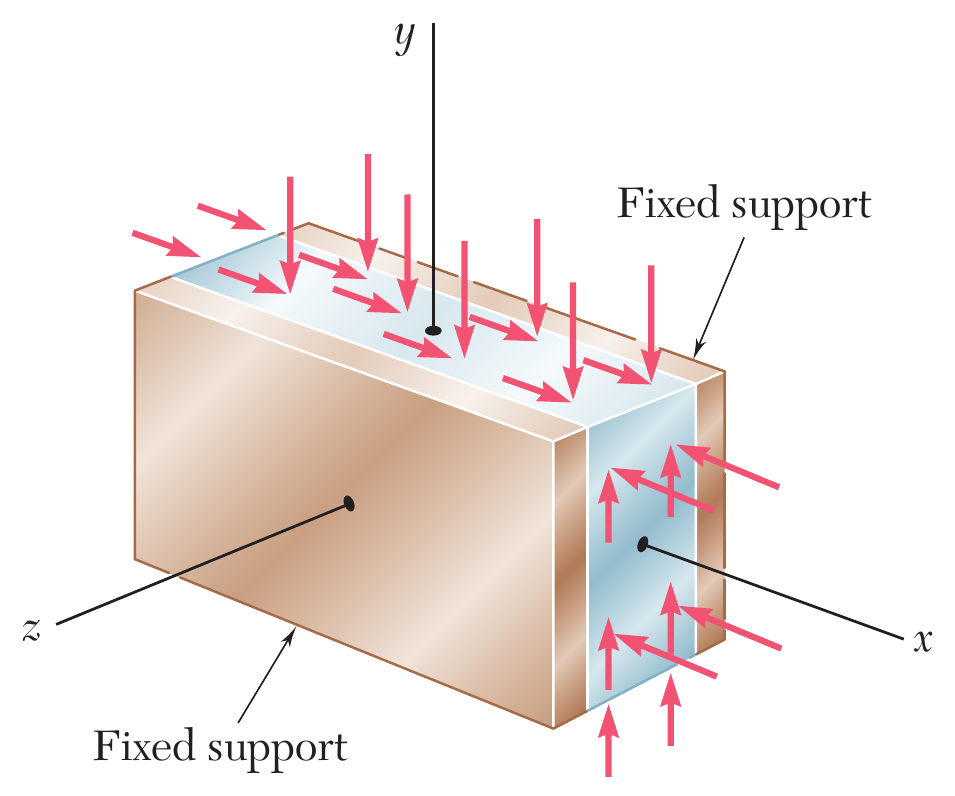
\includegraphics[width=\linewidth,height=2.9cm,keepaspectratio]{Chap_7/fig_7_54.png}\\[2pt]
      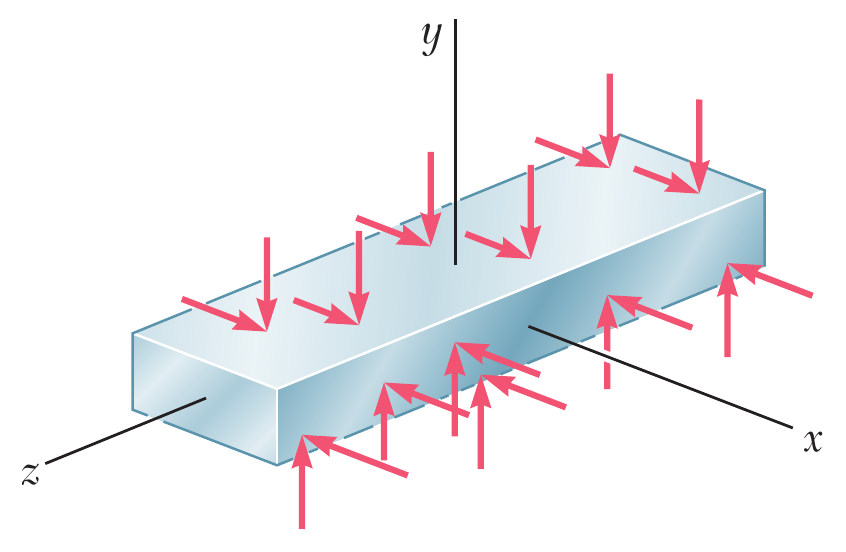
\includegraphics[width=\linewidth,height=2.9cm,keepaspectratio]{Chap_7/fig_7_55.png}
  \end{columns}
\end{frame}
% ===========
\begin{frame}[t]{Biến đổi biến dạng phẳng (tiếp)}
  \begin{columns}[T]
    \column{0.60\textwidth}
      \footnotesize
      \begin{itemize}
        \setlength{\itemsep}{0.3em}
        \item Trạng thái biến dạng tại điểm $Q$ cho các thành phần biến dạng
              khác nhau đối với hệ quy chiếu $xy$ và $x'y'$:
        \[
          \varepsilon(\theta) = \varepsilon_x\cos^2\theta + \varepsilon_y\sin^2\theta
            + \gamma_{xy}\sin\theta\cos\theta
        \]
        \[
          \varepsilon_{OB} = \varepsilon(45^\circ)
            = \tfrac{1}{2}\left(\varepsilon_x + \varepsilon_y + \gamma_{xy}\right)
          \qquad
          \gamma_{xy} = 2\varepsilon_{OB} - (\varepsilon_x + \varepsilon_y)
        \]
        \item Áp dụng các hệ thức lượng giác đã dùng cho biến đổi ứng suất:
      \end{itemize}
      \[
        \begin{aligned}
          \varepsilon_{x'} &= \frac{\varepsilon_x + \varepsilon_y}{2}
            + \frac{\varepsilon_x - \varepsilon_y}{2}\cos2\theta
            + \frac{\gamma_{xy}}{2}\sin2\theta\\
          \varepsilon_{y'} &= \frac{\varepsilon_x + \varepsilon_y}{2}
            - \frac{\varepsilon_x - \varepsilon_y}{2}\cos2\theta
            - \frac{\gamma_{xy}}{2}\sin2\theta\\
          \frac{\gamma_{x'y'}}{2} &= -\frac{\varepsilon_x - \varepsilon_y}{2}\sin2\theta
            + \frac{\gamma_{xy}}{2}\cos2\theta
        \end{aligned}
      \]
    \column{0.38\textwidth}
      \centering
      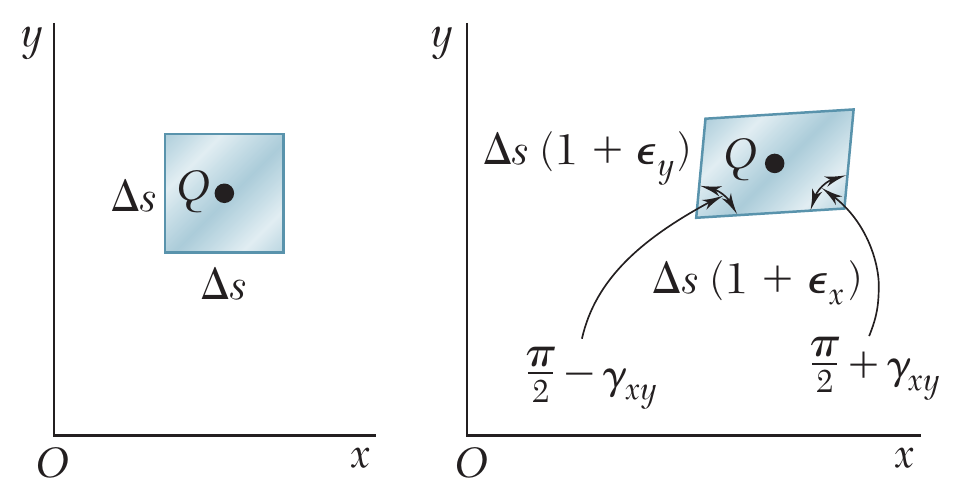
\includegraphics[width=\linewidth,height=2.9cm,keepaspectratio]{Chap_7/fig_7_56.png}\\[2pt]
      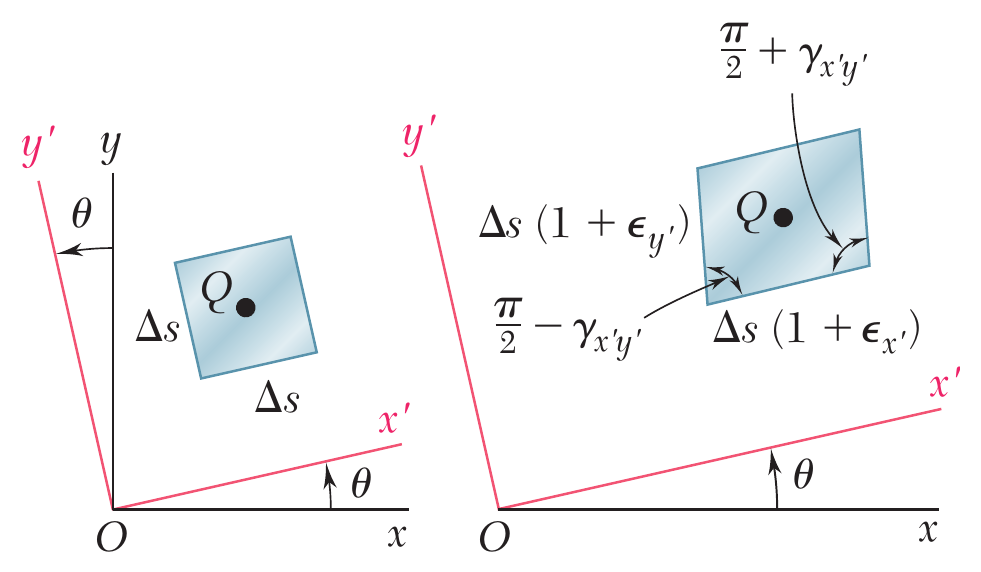
\includegraphics[width=\linewidth,height=2.9cm,keepaspectratio]{Chap_7/fig_7_57.png}
  \end{columns}
\end{frame}
% ===========
\section{Vòng tròn Mohr cho biến dạng phẳng}
\begin{frame}[t]{Vòng tròn Mohr cho biến dạng phẳng}
  \begin{columns}[T]
    \column{0.60\textwidth}
      \small
      \begin{itemize}
        \setlength{\itemsep}{0.4em}
        \item Các phương trình biến đổi biến dạng phẳng có cùng dạng với các
              phương trình biến đổi ứng suất phẳng -- có thể áp dụng kỹ thuật
              vòng tròn Mohr.
        \item Hoành độ tâm $C$ và bán kính $R$:
        \[
          \varepsilon_{\mathrm{tb}} = \frac{\varepsilon_x + \varepsilon_y}{2}
          \qquad
          R = \sqrt{\left(\frac{\varepsilon_x - \varepsilon_y}{2}\right)^2
              + \left(\frac{\gamma_{xy}}{2}\right)^2}
        \]
        \item Các trục chính của biến dạng và các biến dạng chính:
        \[
          \tan2\theta_p = \frac{\gamma_{xy}}{\varepsilon_x - \varepsilon_y}
          \qquad
          \varepsilon_{\max} = \varepsilon_{\mathrm{tb}} + R
          \qquad
          \varepsilon_{\min} = \varepsilon_{\mathrm{tb}} - R
        \]
        \item Biến dạng trượt lớn nhất trong mặt phẳng:
        \[
          \gamma_{\max} = 2R = \sqrt{(\varepsilon_x - \varepsilon_y)^2 + \gamma_{xy}^2}
        \]
      \end{itemize}
    \column{0.38\textwidth}
      \centering
      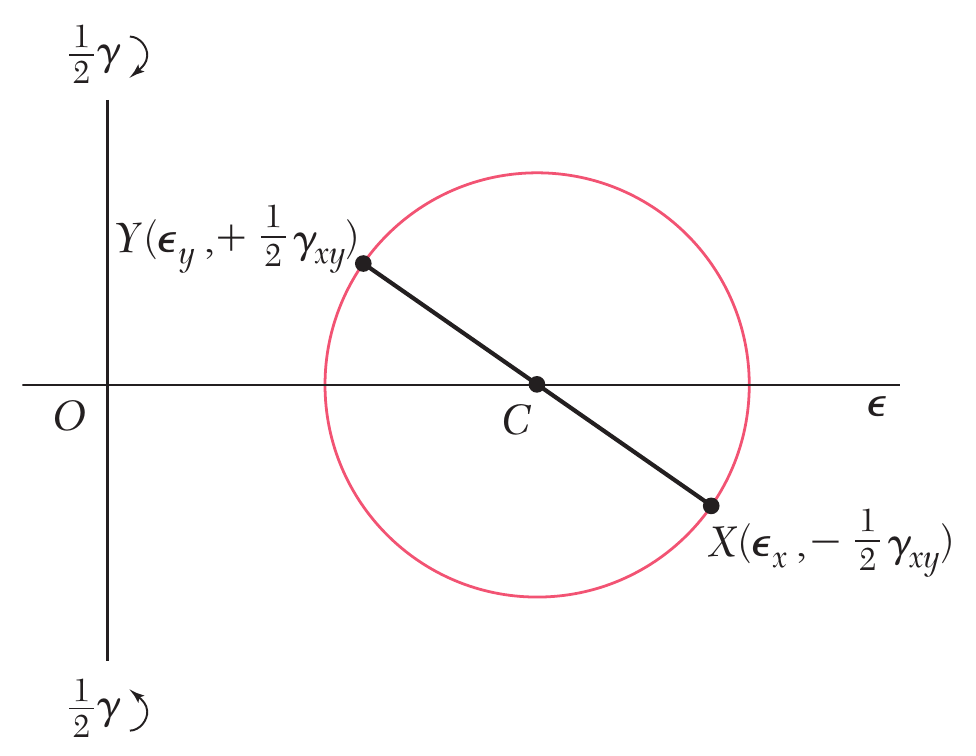
\includegraphics[width=\linewidth,height=2.9cm,keepaspectratio]{Chap_7/fig_7_60.png}\\[2pt]
      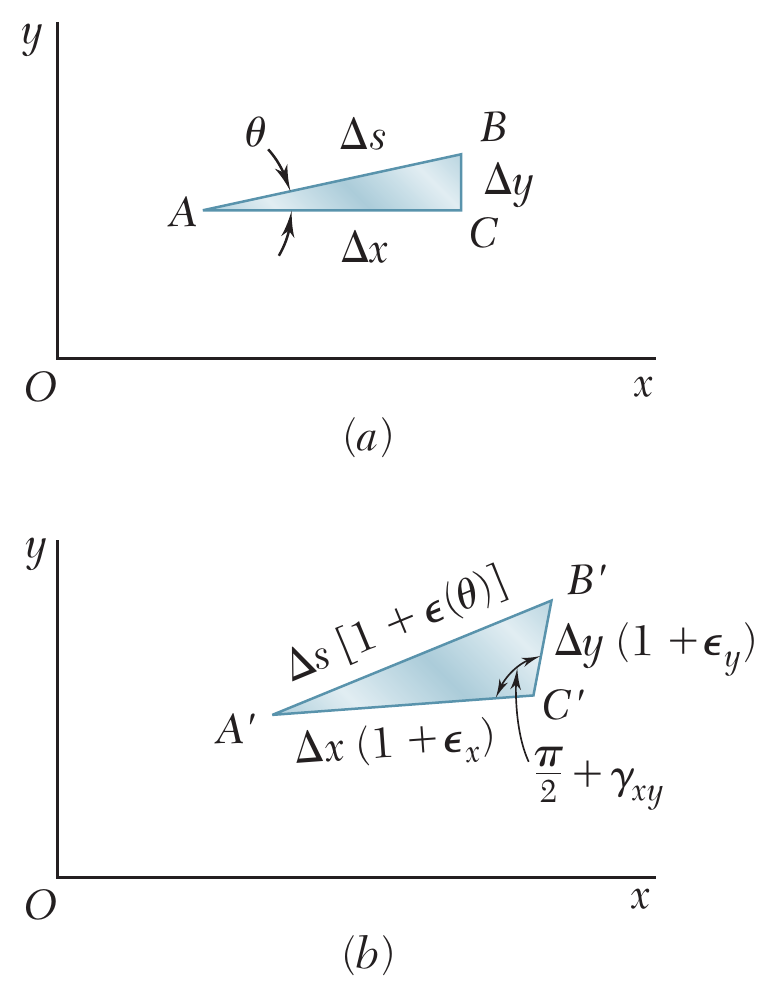
\includegraphics[width=\linewidth,height=2.9cm,keepaspectratio]{Chap_7/fig_7_58.png}
  \end{columns}
\end{frame}
% ===========
\section{Phân tích biến dạng ba chiều}
\begin{frame}[t]{Phân tích biến dạng ba chiều}
  \begin{columns}[T]
    \column{0.56\textwidth}
      \small
      \begin{itemize}
        \setlength{\itemsep}{0.8em}
        \item Như đã chứng minh, tồn tại ba trục chính sao cho các mặt phân tố
              vuông góc với chúng không có ứng suất tiếp.
        \item Theo định luật Hooke, suy ra các biến dạng trượt cũng bằng không,
              và các mặt chính của ứng suất cũng là các mặt chính của biến
              dạng.
        \item Phép xoay quanh các trục chính có thể được biểu diễn bằng các
              vòng tròn Mohr.
      \end{itemize}
    \column{0.42\textwidth}
      \centering
      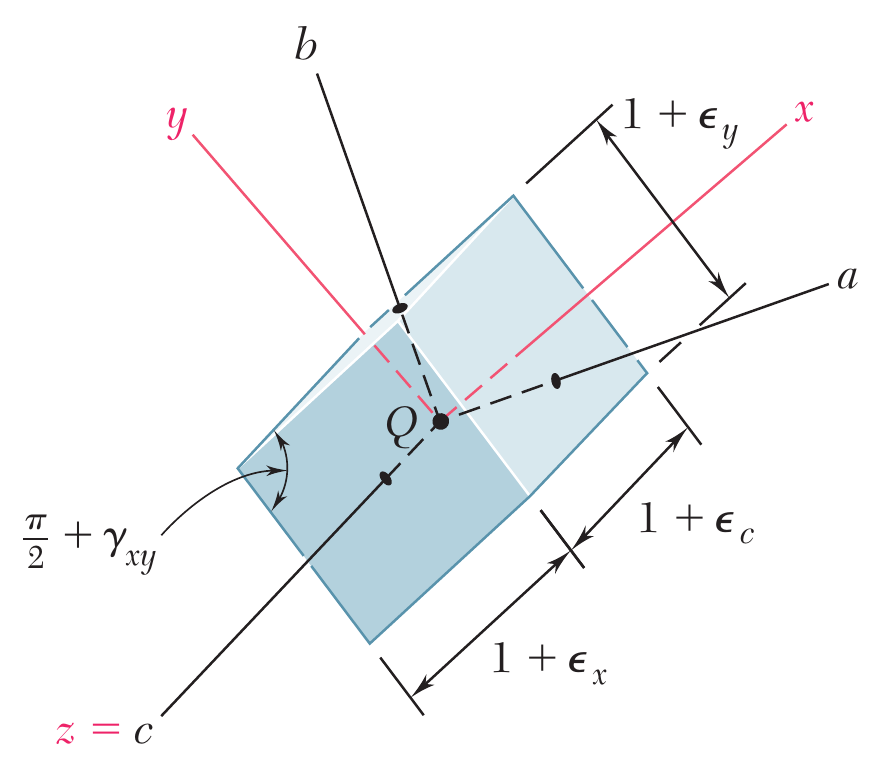
\includegraphics[width=\linewidth,height=2.9cm,keepaspectratio]{Chap_7/fig_7_68.png}\\[2pt]
      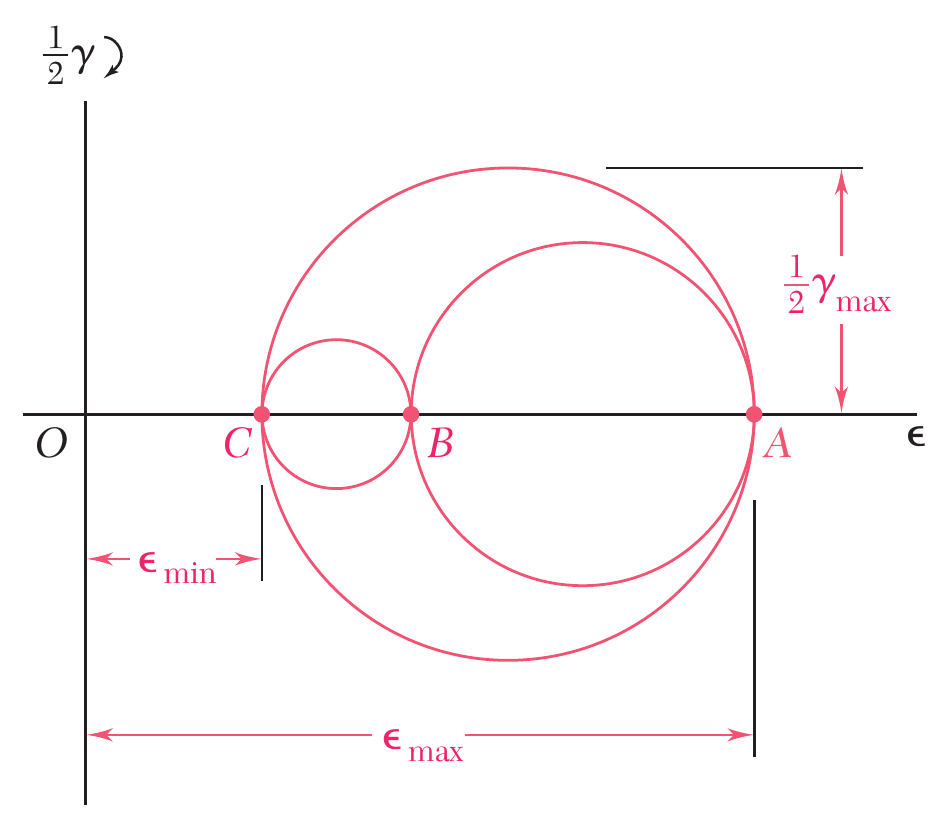
\includegraphics[width=\linewidth,height=2.9cm,keepaspectratio]{Chap_7/fig_7_69.png}
  \end{columns}
\end{frame}
% ===========
\begin{frame}[t]{Phân tích biến dạng ba chiều (tiếp)}
  \begin{columns}[T]
    \column{0.58\textwidth}
      \small
      \begin{itemize}
        \setlength{\itemsep}{0.5em}
        \item Với trường hợp biến dạng phẳng, khi các trục $x$ và $y$ nằm
              trong mặt phẳng biến dạng:
              \begin{itemize}
                \item trục $z$ cũng là một trục chính
                \item biến dạng chính tương ứng được biểu diễn bởi điểm
                      $Z = 0$, tức gốc tọa độ.
              \end{itemize}
        \item Nếu các điểm $A$ và $B$ nằm ở hai phía gốc tọa độ, biến dạng
              trượt lớn nhất là biến dạng trượt lớn nhất trong mặt phẳng,
              ứng với $D$ và $E$.
        \item Nếu các điểm $A$ và $B$ nằm cùng phía gốc tọa độ, biến dạng
              trượt lớn nhất nằm ngoài mặt phẳng biến dạng và được biểu diễn
              bởi các điểm $D'$ và $E'$.
      \end{itemize}
    \column{0.40\textwidth}
      \centering
      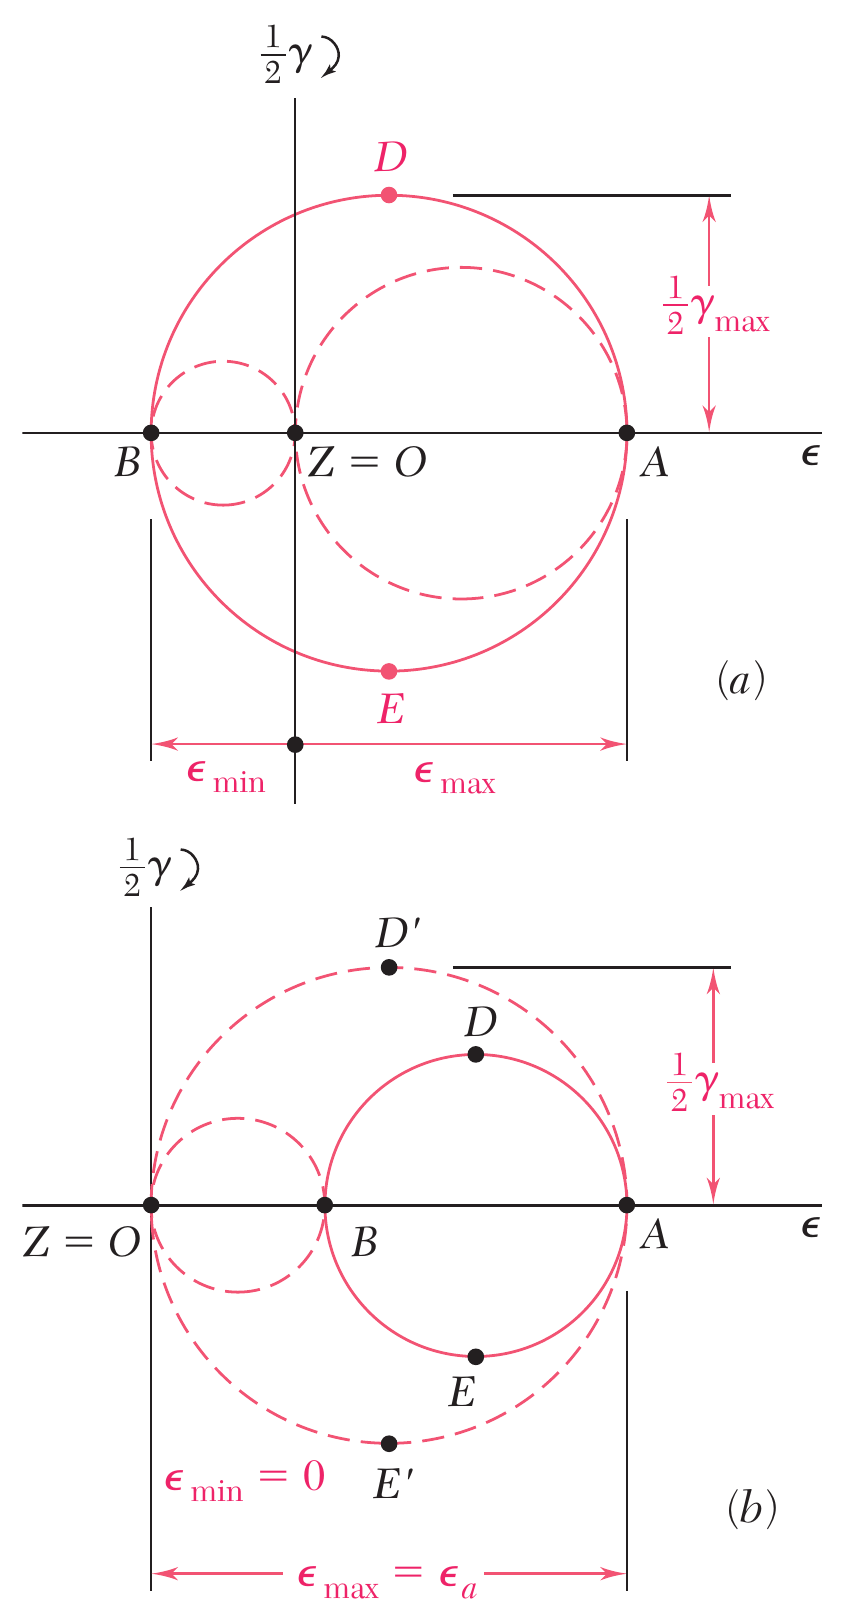
\includegraphics[width=\linewidth,height=2.9cm,keepaspectratio]{Chap_7/fig_7_70.png}\\[2pt]
      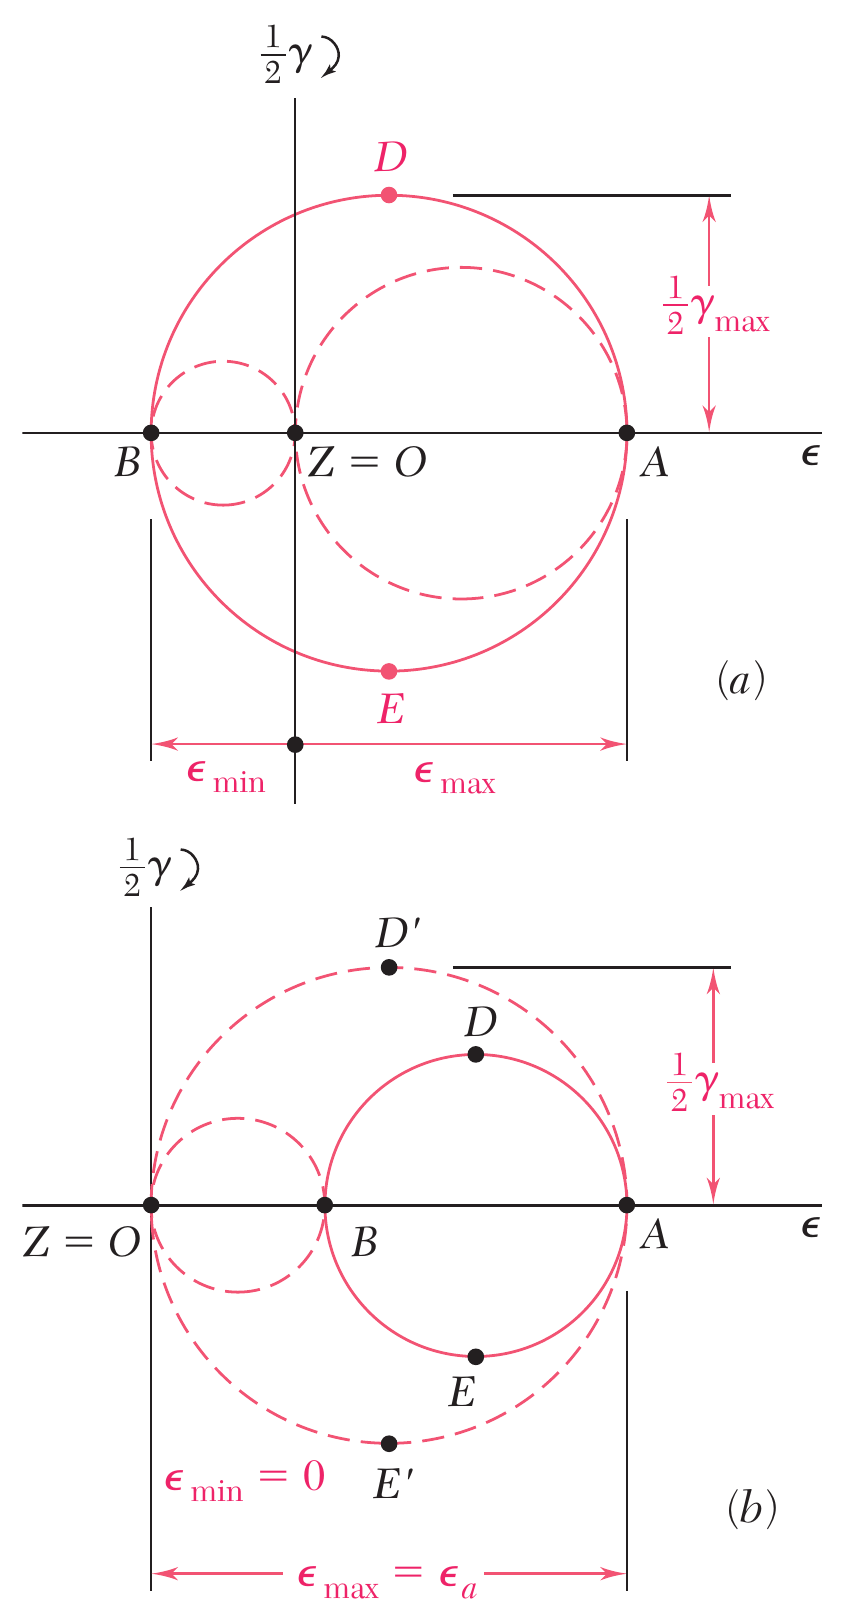
\includegraphics[width=\linewidth,height=2.9cm,keepaspectratio]{Chap_7/fig_7_70.png}
  \end{columns}
\end{frame}
% ===========
\begin{frame}[t]{Phân tích biến dạng ba chiều (tiếp)}
  \begin{columns}[T]
    \column{0.58\textwidth}
      \small
      \begin{itemize}
        \setlength{\itemsep}{0.4em}
        \item Xét trường hợp ứng suất phẳng:
        \[
          \sigma_x = \sigma_a \qquad \sigma_y = \sigma_b \qquad \sigma_z = 0
        \]
        \item Các biến dạng dài tương ứng:
        \[
          \varepsilon_a = +\frac{\sigma_a}{E} - \frac{\nu\sigma_b}{E}
          \qquad
          \varepsilon_b = -\frac{\nu\sigma_a}{E} + \frac{\sigma_b}{E}
        \]
        \[
          \varepsilon_c = -\frac{\nu}{E}(\sigma_a + \sigma_b)
            = -\frac{\nu}{1 - \nu}(\varepsilon_a + \varepsilon_b)
        \]
        \item Biến dạng theo phương vuông góc với mặt phẳng ứng suất khác
              không.
        \item Nếu $B$ nằm giữa $A$ và $C$ trên vòng tròn Mohr, biến dạng
              trượt lớn nhất bằng đường kính $CA$.
      \end{itemize}
    \column{0.40\textwidth}
      \centering
      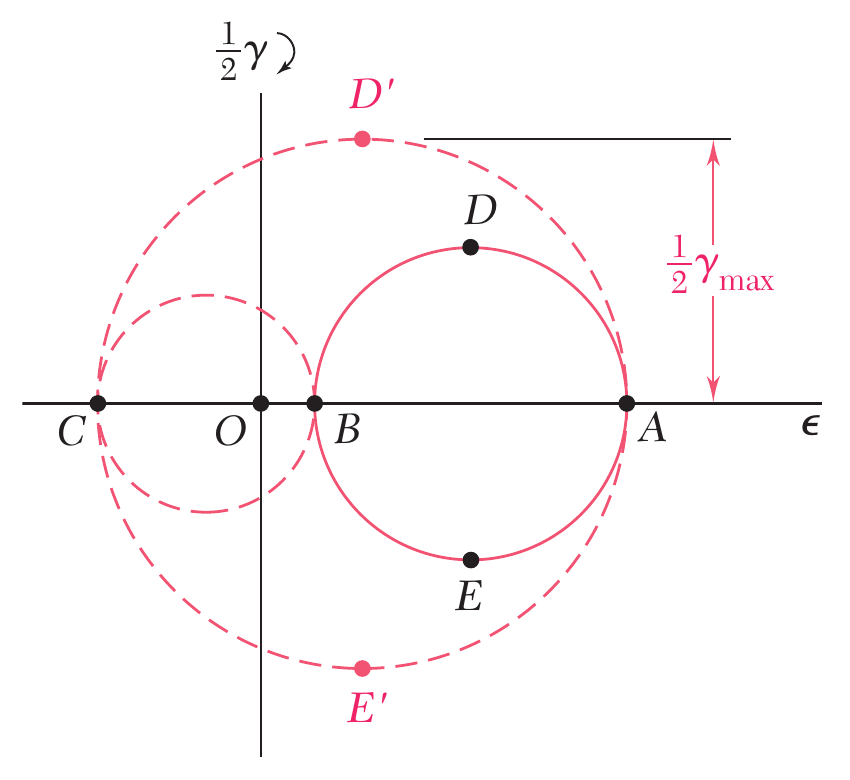
\includegraphics[width=\linewidth,height=5.5cm,keepaspectratio]{Chap_7/fig_7_71.png}
  \end{columns}
\end{frame}
% ===========
\section{Đo biến dạng: cụm cảm biến (rosette)}
\begin{frame}[t]{Đo biến dạng: cụm cảm biến đo biến dạng (rosette)}
  \begin{columns}[T]
    \column{0.60\textwidth}
      \small
      \begin{itemize}
        \setlength{\itemsep}{0.5em}
        \item Cảm biến đo biến dạng (strain gage) cho biết biến dạng dài thông
              qua sự thay đổi điện trở.
        \item Với rosette $45^\circ$, $\varepsilon_x$ và $\varepsilon_y$ được
              đo trực tiếp. $\gamma_{xy}$ được xác định gián tiếp:
        \[
          \gamma_{xy} = 2\varepsilon_{OB} - (\varepsilon_x + \varepsilon_y)
        \]
        \item Biến dạng dài và biến dạng trượt có thể xác định từ biến dạng
              dài theo ba phương bất kỳ:
        \[
          \begin{aligned}
            \varepsilon_1 &= \varepsilon_x\cos^2\theta_1 + \varepsilon_y\sin^2\theta_1
              + \gamma_{xy}\sin\theta_1\cos\theta_1\\
            \varepsilon_2 &= \varepsilon_x\cos^2\theta_2 + \varepsilon_y\sin^2\theta_2
              + \gamma_{xy}\sin\theta_2\cos\theta_2\\
            \varepsilon_3 &= \varepsilon_x\cos^2\theta_3 + \varepsilon_y\sin^2\theta_3
              + \gamma_{xy}\sin\theta_3\cos\theta_3
          \end{aligned}
        \]
      \end{itemize}
    \column{0.38\textwidth}
      \centering
      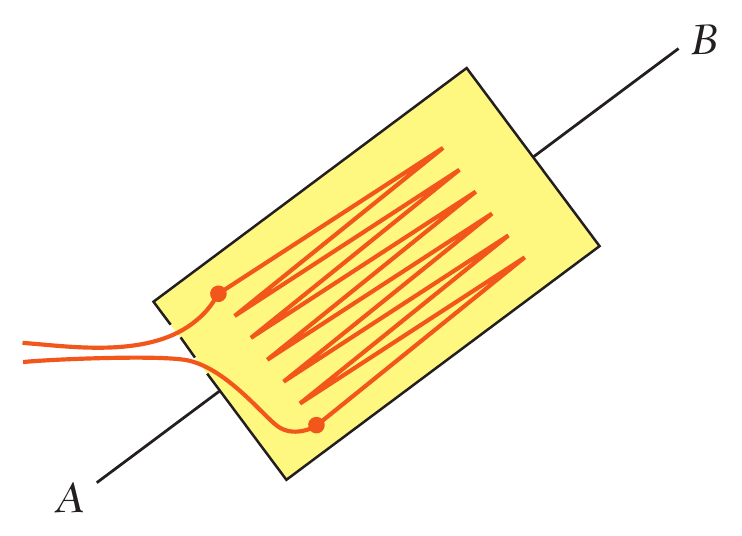
\includegraphics[width=\linewidth,height=2.9cm,keepaspectratio]{Chap_7/fig_7_74.png}\\[2pt]
      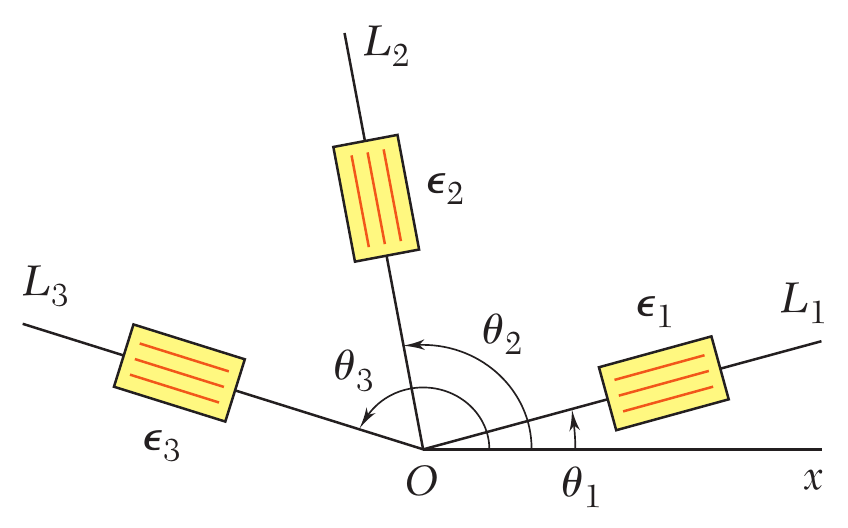
\includegraphics[width=\linewidth,height=2.9cm,keepaspectratio]{Chap_7/fig_7_76.png}
  \end{columns}
\end{frame}

\end{document}
